\documentclass[twoside]{book}

% Packages required by doxygen
\usepackage{calc}
\usepackage{doxygen}
\usepackage{graphicx}
\usepackage[utf8]{inputenc}
\usepackage{makeidx}
\usepackage{multicol}
\usepackage{multirow}
\usepackage{textcomp}
\usepackage[table]{xcolor}

% Font selection
\usepackage[T1]{fontenc}
\usepackage{mathptmx}
\usepackage[scaled=.90]{helvet}
\usepackage{courier}
\usepackage{amssymb}
\usepackage{sectsty}
\renewcommand{\familydefault}{\sfdefault}
\allsectionsfont{%
  \fontseries{bc}\selectfont%
  \color{darkgray}%
}
\renewcommand{\DoxyLabelFont}{%
  \fontseries{bc}\selectfont%
  \color{darkgray}%
}

% Page & text layout
\usepackage{geometry}
\geometry{%
  a4paper,%
  top=2.5cm,%
  bottom=2.5cm,%
  left=2.5cm,%
  right=2.5cm%
}
\tolerance=750
\hfuzz=15pt
\hbadness=750
\setlength{\emergencystretch}{15pt}
\setlength{\parindent}{0cm}
\setlength{\parskip}{0.2cm}
\makeatletter
\renewcommand{\paragraph}{%
  \@startsection{paragraph}{4}{0ex}{-1.0ex}{1.0ex}{%
    \normalfont\normalsize\bfseries\SS@parafont%
  }%
}
\renewcommand{\subparagraph}{%
  \@startsection{subparagraph}{5}{0ex}{-1.0ex}{1.0ex}{%
    \normalfont\normalsize\bfseries\SS@subparafont%
  }%
}
\makeatother

% Headers & footers
\usepackage{fancyhdr}
\pagestyle{fancyplain}
\fancyhead[LE]{\fancyplain{}{\bfseries\thepage}}
\fancyhead[CE]{\fancyplain{}{}}
\fancyhead[RE]{\fancyplain{}{\bfseries\leftmark}}
\fancyhead[LO]{\fancyplain{}{\bfseries\rightmark}}
\fancyhead[CO]{\fancyplain{}{}}
\fancyhead[RO]{\fancyplain{}{\bfseries\thepage}}
\fancyfoot[LE]{\fancyplain{}{}}
\fancyfoot[CE]{\fancyplain{}{}}
\fancyfoot[RE]{\fancyplain{}{\bfseries\scriptsize Generated on Sun May 17 2015 19\-:32\-:34 for P\-A\-M\-S\-I L\-A\-B V\-I\-I by Doxygen }}
\fancyfoot[LO]{\fancyplain{}{\bfseries\scriptsize Generated on Sun May 17 2015 19\-:32\-:34 for P\-A\-M\-S\-I L\-A\-B V\-I\-I by Doxygen }}
\fancyfoot[CO]{\fancyplain{}{}}
\fancyfoot[RO]{\fancyplain{}{}}
\renewcommand{\footrulewidth}{0.4pt}
\renewcommand{\chaptermark}[1]{%
  \markboth{#1}{}%
}
\renewcommand{\sectionmark}[1]{%
  \markright{\thesection\ #1}%
}

% Indices & bibliography
\usepackage{natbib}
\usepackage[titles]{tocloft}
\setcounter{tocdepth}{3}
\setcounter{secnumdepth}{5}
\makeindex

% Hyperlinks (required, but should be loaded last)
\usepackage{ifpdf}
\ifpdf
  \usepackage[pdftex,pagebackref=true]{hyperref}
\else
  \usepackage[ps2pdf,pagebackref=true]{hyperref}
\fi
\hypersetup{%
  colorlinks=true,%
  linkcolor=blue,%
  citecolor=blue,%
  unicode%
}

% Custom commands
\newcommand{\clearemptydoublepage}{%
  \newpage{\pagestyle{empty}\cleardoublepage}%
}


%===== C O N T E N T S =====

\begin{document}

% Titlepage & ToC
\hypersetup{pageanchor=false}
\pagenumbering{roman}
\begin{titlepage}
\vspace*{7cm}
\begin{center}%
{\Large P\-A\-M\-S\-I L\-A\-B V\-I\-I }\\
\vspace*{1cm}
{\large Generated by Doxygen 1.8.6}\\
\vspace*{0.5cm}
{\small Sun May 17 2015 19:32:34}\\
\end{center}
\end{titlepage}
\clearemptydoublepage
\tableofcontents
\clearemptydoublepage
\pagenumbering{arabic}
\hypersetup{pageanchor=true}

%--- Begin generated contents ---
\chapter{Hierarchical Index}
\subsection{Class Hierarchy}
This inheritance list is sorted roughly, but not completely, alphabetically\-:\begin{DoxyCompactList}
\item \contentsline{section}{Benchmark$<$ typ $>$}{\pageref{class_benchmark}}{}
\item \contentsline{section}{Kolejka$<$ typ $>$\-:\-:Element}{\pageref{struct_kolejka_1_1_element}}{}
\item \contentsline{section}{Lista$<$ typ $>$\-:\-:Element}{\pageref{struct_lista_1_1_element}}{}
\item \contentsline{section}{Stos$<$ typ $>$\-:\-:Element}{\pageref{struct_stos_1_1_element}}{}
\item \contentsline{section}{Framework}{\pageref{class_framework}}{}
\begin{DoxyCompactList}
\item \contentsline{section}{Interfejs\-A\-D\-T$<$ typ $>$}{\pageref{class_interfejs_a_d_t}}{}
\begin{DoxyCompactList}
\item \contentsline{section}{Kolejka$<$ typ $>$}{\pageref{class_kolejka}}{}
\item \contentsline{section}{Lista$<$ typ $>$}{\pageref{class_lista}}{}
\item \contentsline{section}{List\-Arr1$<$ typ $>$}{\pageref{class_list_arr1}}{}
\item \contentsline{section}{List\-Arr2x$<$ typ $>$}{\pageref{class_list_arr2x}}{}
\item \contentsline{section}{Stos$<$ typ $>$}{\pageref{class_stos}}{}
\end{DoxyCompactList}
\end{DoxyCompactList}
\item \contentsline{section}{Statystyka}{\pageref{class_statystyka}}{}
\end{DoxyCompactList}

\chapter{Class Index}
\subsection{Class List}
Here are the classes, structs, unions and interfaces with brief descriptions\-:\begin{DoxyCompactList}
\item\contentsline{section}{\hyperlink{class_benchmark}{Benchmark$<$ typ $>$} \\*Modeluje pojęcie Benchmarku }{\pageref{class_benchmark}}{}
\item\contentsline{section}{\hyperlink{struct_kolejka_1_1_element}{Kolejka$<$ typ $>$\-::\-Element} \\*Modeluje jeden element Kolejki }{\pageref{struct_kolejka_1_1_element}}{}
\item\contentsline{section}{\hyperlink{struct_lista_1_1_element}{Lista$<$ typ $>$\-::\-Element} \\*Modeluje jeden element Listy }{\pageref{struct_lista_1_1_element}}{}
\item\contentsline{section}{\hyperlink{struct_stos_1_1_element}{Stos$<$ typ $>$\-::\-Element} \\*Modeluje jeden element Stosu }{\pageref{struct_stos_1_1_element}}{}
\item\contentsline{section}{\hyperlink{class_framework}{Framework} \\*Modeluje interfejs programu }{\pageref{class_framework}}{}
\item\contentsline{section}{\hyperlink{class_interfejs_a_d_t}{Interfejs\-A\-D\-T$<$ typ $>$} }{\pageref{class_interfejs_a_d_t}}{}
\item\contentsline{section}{\hyperlink{class_kolejka}{Kolejka$<$ typ $>$} \\*Modeluje pojęcie Kolejki }{\pageref{class_kolejka}}{}
\item\contentsline{section}{\hyperlink{class_lista}{Lista$<$ typ $>$} \\*Modeluje pojęcie listy }{\pageref{class_lista}}{}
\item\contentsline{section}{\hyperlink{class_list_arr1}{List\-Arr1$<$ typ $>$} \\*Modeluje pojęcie Listy (array) }{\pageref{class_list_arr1}}{}
\item\contentsline{section}{\hyperlink{class_list_arr2x}{List\-Arr2x$<$ typ $>$} \\*Modeluje pojęcie Listy (array) }{\pageref{class_list_arr2x}}{}
\item\contentsline{section}{\hyperlink{class_statystyka}{Statystyka} \\*Modeluje pojęcie statystyki }{\pageref{class_statystyka}}{}
\item\contentsline{section}{\hyperlink{class_stos}{Stos$<$ typ $>$} \\*Modeluje pojęcie Stosu }{\pageref{class_stos}}{}
\end{DoxyCompactList}

\chapter{File Index}
\section{File List}
Here is a list of all files with brief descriptions\-:\begin{DoxyCompactList}
\item\contentsline{section}{/home/bartolomeo/209296/prj/inc/\hyperlink{_benchmark_interfejs_8hh}{Benchmark\-Interfejs.\-hh} }{\pageref{_benchmark_interfejs_8hh}}{}
\item\contentsline{section}{/home/bartolomeo/209296/prj/inc/\hyperlink{_czasomierz_8hh}{Czasomierz.\-hh} }{\pageref{_czasomierz_8hh}}{}
\item\contentsline{section}{/home/bartolomeo/209296/prj/inc/\hyperlink{_h_sort_8hh}{H\-Sort.\-hh} }{\pageref{_h_sort_8hh}}{}
\item\contentsline{section}{/home/bartolomeo/209296/prj/inc/\hyperlink{_hyb_sort_8hh}{Hyb\-Sort.\-hh} }{\pageref{_hyb_sort_8hh}}{}
\item\contentsline{section}{/home/bartolomeo/209296/prj/inc/\hyperlink{_i_obserwator_8hh}{I\-Obserwator.\-hh} }{\pageref{_i_obserwator_8hh}}{}
\item\contentsline{section}{/home/bartolomeo/209296/prj/inc/\hyperlink{_i_obserwowany_8hh}{I\-Obserwowany.\-hh} }{\pageref{_i_obserwowany_8hh}}{}
\item\contentsline{section}{/home/bartolomeo/209296/prj/inc/\hyperlink{_i_sortable_8hh}{I\-Sortable.\-hh} }{\pageref{_i_sortable_8hh}}{}
\item\contentsline{section}{/home/bartolomeo/209296/prj/inc/\hyperlink{_i_struktury_8hh}{I\-Struktury.\-hh} }{\pageref{_i_struktury_8hh}}{}
\item\contentsline{section}{/home/bartolomeo/209296/prj/inc/\hyperlink{_iterable_8hh}{Iterable.\-hh} }{\pageref{_iterable_8hh}}{}
\item\contentsline{section}{/home/bartolomeo/209296/prj/inc/\hyperlink{_list_arr2x_8hh}{List\-Arr2x.\-hh} \\*Definicja klasy List\-Arr1 }{\pageref{_list_arr2x_8hh}}{}
\item\contentsline{section}{/home/bartolomeo/209296/prj/inc/\hyperlink{_m_sort_8hh}{M\-Sort.\-hh} }{\pageref{_m_sort_8hh}}{}
\item\contentsline{section}{/home/bartolomeo/209296/prj/inc/\hyperlink{_q_sort_8hh}{Q\-Sort.\-hh} }{\pageref{_q_sort_8hh}}{}
\item\contentsline{section}{/home/bartolomeo/209296/prj/inc/\hyperlink{_q_sort_opt_8hh}{Q\-Sort\-Opt.\-hh} }{\pageref{_q_sort_opt_8hh}}{}
\item\contentsline{section}{/home/bartolomeo/209296/prj/inc/\hyperlink{_stos_tab_8hh}{Stos\-Tab.\-hh} }{\pageref{_stos_tab_8hh}}{}
\item\contentsline{section}{/home/bartolomeo/209296/prj/inc/\hyperlink{_struktury_benchmark_8hh}{Struktury\-Benchmark.\-hh} }{\pageref{_struktury_benchmark_8hh}}{}
\item\contentsline{section}{/home/bartolomeo/209296/prj/inc/\hyperlink{_wyniki_8hh}{Wyniki.\-hh} }{\pageref{_wyniki_8hh}}{}
\item\contentsline{section}{/home/bartolomeo/209296/prj/src/\hyperlink{_czasomierz_8cpp}{Czasomierz.\-cpp} }{\pageref{_czasomierz_8cpp}}{}
\item\contentsline{section}{/home/bartolomeo/209296/prj/src/\hyperlink{_main_8cpp}{Main.\-cpp} \\*Funkcja glowna programu }{\pageref{_main_8cpp}}{}
\item\contentsline{section}{/home/bartolomeo/209296/prj/src/\hyperlink{_wyniki_8cpp}{Wyniki.\-cpp} }{\pageref{_wyniki_8cpp}}{}
\end{DoxyCompactList}

\chapter{Class Documentation}
\hypertarget{class_benchmark_interfejs}{\section{Benchmark\-Interfejs Class Reference}
\label{class_benchmark_interfejs}\index{Benchmark\-Interfejs@{Benchmark\-Interfejs}}
}


Modeluje pojecie Interfejsu Benchmark'u.  




{\ttfamily \#include $<$Benchmark\-Interfejs.\-hh$>$}

Inheritance diagram for Benchmark\-Interfejs\-:\begin{figure}[H]
\begin{center}
\leavevmode
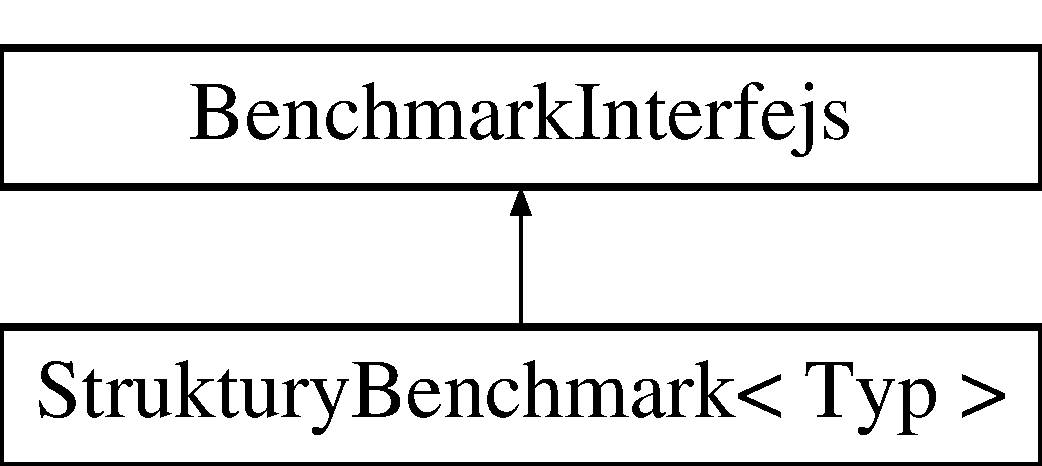
\includegraphics[height=2.000000cm]{class_benchmark_interfejs}
\end{center}
\end{figure}
\subsection*{Protected Member Functions}
\begin{DoxyCompactItemize}
\item 
virtual void \hyperlink{class_benchmark_interfejs_a614b8d69d8af00260210da6308769947}{\-\_\-\-Test} () const =0
\begin{DoxyCompactList}\small\item\em Metoda Wykonujaca pojedyncza operacje. \end{DoxyCompactList}\item 
virtual void \hyperlink{class_benchmark_interfejs_a7980830be212d0ea0ffd2e12b083cd06}{\-\_\-\-Wczytaj} (string Plik\-Wart)=0
\begin{DoxyCompactList}\small\item\em Metoda wczytujaca dane z pliku Metoda ma za zadanie wczytac dane z pliku wejsciowego. \end{DoxyCompactList}\item 
virtual void \hyperlink{class_benchmark_interfejs_a25ad3aa17a7faa3489d82b9f7c763cce}{\-\_\-\-Zaladuj} (const unsigned int n) const =0
\begin{DoxyCompactList}\small\item\em Metoda wypelniajaca Metoda ma za zadanie wypelnic dany kontener danymi. \end{DoxyCompactList}\item 
virtual void \hyperlink{class_benchmark_interfejs_a8a1165914a09368530183ffb968541f1}{\-\_\-\-Zwolnij} ()=0
\begin{DoxyCompactList}\small\item\em Metoda zwalniajaca Pamiec. \end{DoxyCompactList}\item 
virtual void \hyperlink{class_benchmark_interfejs_a69c431ffaa9d2ab995458cc8c6ae5c1f}{\-\_\-\-Generator} () const =0
\begin{DoxyCompactList}\small\item\em Metoda generujaca dane. \end{DoxyCompactList}\end{DoxyCompactItemize}


\subsection{Detailed Description}
Modeluje pojecie Interfejsu Benchmark'u. 

Klasa bazowa dla implementowania benchmarku dla kolejnych struktur danych 

\subsection{Member Function Documentation}
\hypertarget{class_benchmark_interfejs_a69c431ffaa9d2ab995458cc8c6ae5c1f}{\index{Benchmark\-Interfejs@{Benchmark\-Interfejs}!\-\_\-\-Generator@{\-\_\-\-Generator}}
\index{\-\_\-\-Generator@{\-\_\-\-Generator}!BenchmarkInterfejs@{Benchmark\-Interfejs}}
\subsubsection[{\-\_\-\-Generator}]{\setlength{\rightskip}{0pt plus 5cm}virtual void Benchmark\-Interfejs\-::\-\_\-\-Generator (
\begin{DoxyParamCaption}
{}
\end{DoxyParamCaption}
) const\hspace{0.3cm}{\ttfamily [protected]}, {\ttfamily [pure virtual]}}}\label{class_benchmark_interfejs_a69c431ffaa9d2ab995458cc8c6ae5c1f}


Metoda generujaca dane. 

Metoda ma za zadanie wygenerowac pseudolosowe dane i zapisac je do pliku 

Implemented in \hyperlink{class_struktury_benchmark_aa5a6c92b86be3cd99177322c92329164}{Struktury\-Benchmark$<$ Typ $>$}.

\hypertarget{class_benchmark_interfejs_a614b8d69d8af00260210da6308769947}{\index{Benchmark\-Interfejs@{Benchmark\-Interfejs}!\-\_\-\-Test@{\-\_\-\-Test}}
\index{\-\_\-\-Test@{\-\_\-\-Test}!BenchmarkInterfejs@{Benchmark\-Interfejs}}
\subsubsection[{\-\_\-\-Test}]{\setlength{\rightskip}{0pt plus 5cm}virtual void Benchmark\-Interfejs\-::\-\_\-\-Test (
\begin{DoxyParamCaption}
{}
\end{DoxyParamCaption}
) const\hspace{0.3cm}{\ttfamily [protected]}, {\ttfamily [pure virtual]}}}\label{class_benchmark_interfejs_a614b8d69d8af00260210da6308769947}


Metoda Wykonujaca pojedyncza operacje. 

Metoda ma za zadanie wykonan pojedyncza operacja, ktorej czas jest rejestrowany 
\begin{DoxyParams}[1]{Parameters}
\mbox{\tt in}  & {\em Ilosc} & -\/ Liczba danych poddana testowi \\
\hline
\end{DoxyParams}


Implemented in \hyperlink{class_struktury_benchmark_a437a5c4b2a1811f3067d1117ac2c2c0e}{Struktury\-Benchmark$<$ Typ $>$}.

\hypertarget{class_benchmark_interfejs_a7980830be212d0ea0ffd2e12b083cd06}{\index{Benchmark\-Interfejs@{Benchmark\-Interfejs}!\-\_\-\-Wczytaj@{\-\_\-\-Wczytaj}}
\index{\-\_\-\-Wczytaj@{\-\_\-\-Wczytaj}!BenchmarkInterfejs@{Benchmark\-Interfejs}}
\subsubsection[{\-\_\-\-Wczytaj}]{\setlength{\rightskip}{0pt plus 5cm}virtual void Benchmark\-Interfejs\-::\-\_\-\-Wczytaj (
\begin{DoxyParamCaption}
\item[{string}]{Plik\-Wart}
\end{DoxyParamCaption}
)\hspace{0.3cm}{\ttfamily [protected]}, {\ttfamily [pure virtual]}}}\label{class_benchmark_interfejs_a7980830be212d0ea0ffd2e12b083cd06}


Metoda wczytujaca dane z pliku Metoda ma za zadanie wczytac dane z pliku wejsciowego. 


\begin{DoxyParams}[1]{Parameters}
\mbox{\tt in}  & {\em Plik\-In} & -\/ Nazwa pliku wejsciowego \\
\hline
\mbox{\tt in}  & {\em n} & -\/ liczba wczytywanych danych \\
\hline
\end{DoxyParams}


Implemented in \hyperlink{class_struktury_benchmark_a949e7eef56ff1dce1be1afac5fccc306}{Struktury\-Benchmark$<$ Typ $>$}.

\hypertarget{class_benchmark_interfejs_a25ad3aa17a7faa3489d82b9f7c763cce}{\index{Benchmark\-Interfejs@{Benchmark\-Interfejs}!\-\_\-\-Zaladuj@{\-\_\-\-Zaladuj}}
\index{\-\_\-\-Zaladuj@{\-\_\-\-Zaladuj}!BenchmarkInterfejs@{Benchmark\-Interfejs}}
\subsubsection[{\-\_\-\-Zaladuj}]{\setlength{\rightskip}{0pt plus 5cm}virtual void Benchmark\-Interfejs\-::\-\_\-\-Zaladuj (
\begin{DoxyParamCaption}
\item[{const unsigned int}]{n}
\end{DoxyParamCaption}
) const\hspace{0.3cm}{\ttfamily [protected]}, {\ttfamily [pure virtual]}}}\label{class_benchmark_interfejs_a25ad3aa17a7faa3489d82b9f7c763cce}


Metoda wypelniajaca Metoda ma za zadanie wypelnic dany kontener danymi. 


\begin{DoxyParams}[1]{Parameters}
\mbox{\tt in}  & {\em n} & -\/ ilosc danych \\
\hline
\end{DoxyParams}


Implemented in \hyperlink{class_struktury_benchmark_a263ee44187c7efb212d031e97cd39bb1}{Struktury\-Benchmark$<$ Typ $>$}.

\hypertarget{class_benchmark_interfejs_a8a1165914a09368530183ffb968541f1}{\index{Benchmark\-Interfejs@{Benchmark\-Interfejs}!\-\_\-\-Zwolnij@{\-\_\-\-Zwolnij}}
\index{\-\_\-\-Zwolnij@{\-\_\-\-Zwolnij}!BenchmarkInterfejs@{Benchmark\-Interfejs}}
\subsubsection[{\-\_\-\-Zwolnij}]{\setlength{\rightskip}{0pt plus 5cm}virtual void Benchmark\-Interfejs\-::\-\_\-\-Zwolnij (
\begin{DoxyParamCaption}
{}
\end{DoxyParamCaption}
)\hspace{0.3cm}{\ttfamily [protected]}, {\ttfamily [pure virtual]}}}\label{class_benchmark_interfejs_a8a1165914a09368530183ffb968541f1}


Metoda zwalniajaca Pamiec. 

Metoda ma za zadanie zwolnic pamiec przeznaczona na dane przechowywane w kontenerze 

Implemented in \hyperlink{class_struktury_benchmark_a81596424109f9dbe028c3ad3496d04a1}{Struktury\-Benchmark$<$ Typ $>$}.



The documentation for this class was generated from the following file\-:\begin{DoxyCompactItemize}
\item 
/home/bartolomeo/209296/prj/inc/\hyperlink{_benchmark_interfejs_8hh}{Benchmark\-Interfejs.\-hh}\end{DoxyCompactItemize}

\hypertarget{class_czasomierz}{\section{Czasomierz Class Reference}
\label{class_czasomierz}\index{Czasomierz@{Czasomierz}}
}


Modeluje pojecie Czasomierza.  




{\ttfamily \#include $<$Czasomierz.\-hh$>$}

\subsection*{Public Member Functions}
\begin{DoxyCompactItemize}
\item 
\hyperlink{class_czasomierz_aa49ccbbc365ff5e54b41f4ec4d769038}{Czasomierz} ()
\begin{DoxyCompactList}\small\item\em Konstruktor obiektu. \end{DoxyCompactList}\item 
void \hyperlink{class_czasomierz_a26f594c73a3b382d1695f14a5682ca7c}{\-\_\-\-Rozpocznij\-Pomiar} ()
\begin{DoxyCompactList}\small\item\em Metoda zaczynajaca pomiar. \end{DoxyCompactList}\item 
void \hyperlink{class_czasomierz_a91e1a8e33b5e1eb7a5036eed57fb13a3}{\-\_\-\-Zakoncz\-Pomiar} ()
\begin{DoxyCompactList}\small\item\em Metoda konczaca pomiar. \end{DoxyCompactList}\item 
void \hyperlink{class_czasomierz_aecc4b89376b85367ab0e44fecb4ca6df}{\-\_\-\-Aktualizuj\-Czas} ()
\begin{DoxyCompactList}\small\item\em Metoda Aktualizujaca czas danej proby. \end{DoxyCompactList}\item 
long double \hyperlink{class_czasomierz_a80be3a3d837f8ca28e1a6bc2f231f0d7}{\-\_\-\-Czas\-Trwania} () const 
\begin{DoxyCompactList}\small\item\em Metoda zwracajaca calkowity czas Proby. \end{DoxyCompactList}\item 
void \hyperlink{class_czasomierz_a1f2c55e5be7f93f3db9b02eb5757cc78}{\-\_\-\-Reset} ()
\begin{DoxyCompactList}\small\item\em Metoda resetujaca \hyperlink{class_czasomierz}{Czasomierz}. \end{DoxyCompactList}\item 
bool \hyperlink{class_czasomierz_ab5977fad1080924fe85f70157de7b4db}{\-\_\-\-Status\-Pracy} () const 
\item 
double \hyperlink{class_czasomierz_a02353d27a6e73f00e41c4c0b40990d58}{\-\_\-\-Pojedynczy\-Pomiar} () const 
\begin{DoxyCompactList}\small\item\em Metoda zwracajaca czas pojedynczego pomiaru. \end{DoxyCompactList}\end{DoxyCompactItemize}
\subsection*{Private Attributes}
\begin{DoxyCompactItemize}
\item 
clock\-\_\-t \hyperlink{class_czasomierz_aba798db3d70227410bfafbb01a52d755}{\-\_\-\-Start}
\begin{DoxyCompactList}\small\item\em Pole klasy \hyperlink{class_czasomierz}{Czasomierz}. \end{DoxyCompactList}\item 
clock\-\_\-t \hyperlink{class_czasomierz_a1d791b2017e7f992a2206155982055af}{\-\_\-\-Koniec}
\begin{DoxyCompactList}\small\item\em Pole klasy \hyperlink{class_czasomierz}{Czasomierz}. \end{DoxyCompactList}\item 
long double \hyperlink{class_czasomierz_ae09344cf8ca5613cd557cb4fcf9aa046}{\-\_\-\-Aktualny}
\begin{DoxyCompactList}\small\item\em Pole klasy \hyperlink{class_czasomierz}{Czasomierz}. \end{DoxyCompactList}\item 
bool \hyperlink{class_czasomierz_a5eb9aa3fd9f0fb8af343f2865d490e64}{\-\_\-\-Status}
\begin{DoxyCompactList}\small\item\em Pole klasy \hyperlink{class_czasomierz}{Czasomierz}. \end{DoxyCompactList}\end{DoxyCompactItemize}


\subsection{Detailed Description}
Modeluje pojecie Czasomierza. 

Klasa ma za zadanie mierzyc czas wykonywania danego algorytmu oraz przechowywac informacje o srednich czasach pomiarow dla wybranej ilosci danych przy okreslonej liczbie powtorzen testu 

\subsection{Constructor \& Destructor Documentation}
\hypertarget{class_czasomierz_aa49ccbbc365ff5e54b41f4ec4d769038}{\index{Czasomierz@{Czasomierz}!Czasomierz@{Czasomierz}}
\index{Czasomierz@{Czasomierz}!Czasomierz@{Czasomierz}}
\subsubsection[{Czasomierz}]{\setlength{\rightskip}{0pt plus 5cm}Czasomierz\-::\-Czasomierz (
\begin{DoxyParamCaption}
{}
\end{DoxyParamCaption}
)}}\label{class_czasomierz_aa49ccbbc365ff5e54b41f4ec4d769038}


Konstruktor obiektu. 

Konstruktor klasy \hyperlink{class_czasomierz}{Czasomierz}, zerujacy wszystkie pola tej klasy 

\subsection{Member Function Documentation}
\hypertarget{class_czasomierz_aecc4b89376b85367ab0e44fecb4ca6df}{\index{Czasomierz@{Czasomierz}!\-\_\-\-Aktualizuj\-Czas@{\-\_\-\-Aktualizuj\-Czas}}
\index{\-\_\-\-Aktualizuj\-Czas@{\-\_\-\-Aktualizuj\-Czas}!Czasomierz@{Czasomierz}}
\subsubsection[{\-\_\-\-Aktualizuj\-Czas}]{\setlength{\rightskip}{0pt plus 5cm}void Czasomierz\-::\-\_\-\-Aktualizuj\-Czas (
\begin{DoxyParamCaption}
{}
\end{DoxyParamCaption}
)}}\label{class_czasomierz_aecc4b89376b85367ab0e44fecb4ca6df}


Metoda Aktualizujaca czas danej proby. 

Metoda ma za zadanie zaktualizowac czas danej proby, za sprawa dodadania do poprzedniej sumy pomiarow, czas ktory przypada na najnowszy pomiar \hypertarget{class_czasomierz_a80be3a3d837f8ca28e1a6bc2f231f0d7}{\index{Czasomierz@{Czasomierz}!\-\_\-\-Czas\-Trwania@{\-\_\-\-Czas\-Trwania}}
\index{\-\_\-\-Czas\-Trwania@{\-\_\-\-Czas\-Trwania}!Czasomierz@{Czasomierz}}
\subsubsection[{\-\_\-\-Czas\-Trwania}]{\setlength{\rightskip}{0pt plus 5cm}long double Czasomierz\-::\-\_\-\-Czas\-Trwania (
\begin{DoxyParamCaption}
{}
\end{DoxyParamCaption}
) const}}\label{class_czasomierz_a80be3a3d837f8ca28e1a6bc2f231f0d7}


Metoda zwracajaca calkowity czas Proby. 

Metoda ma za zadanie zwrocic calkowity czas przypadajacy na dana probe \hypertarget{class_czasomierz_a02353d27a6e73f00e41c4c0b40990d58}{\index{Czasomierz@{Czasomierz}!\-\_\-\-Pojedynczy\-Pomiar@{\-\_\-\-Pojedynczy\-Pomiar}}
\index{\-\_\-\-Pojedynczy\-Pomiar@{\-\_\-\-Pojedynczy\-Pomiar}!Czasomierz@{Czasomierz}}
\subsubsection[{\-\_\-\-Pojedynczy\-Pomiar}]{\setlength{\rightskip}{0pt plus 5cm}double Czasomierz\-::\-\_\-\-Pojedynczy\-Pomiar (
\begin{DoxyParamCaption}
{}
\end{DoxyParamCaption}
) const}}\label{class_czasomierz_a02353d27a6e73f00e41c4c0b40990d58}


Metoda zwracajaca czas pojedynczego pomiaru. 

Metoda ma za zadanie zwrocic czas trwania pojedynczego testu \hypertarget{class_czasomierz_a1f2c55e5be7f93f3db9b02eb5757cc78}{\index{Czasomierz@{Czasomierz}!\-\_\-\-Reset@{\-\_\-\-Reset}}
\index{\-\_\-\-Reset@{\-\_\-\-Reset}!Czasomierz@{Czasomierz}}
\subsubsection[{\-\_\-\-Reset}]{\setlength{\rightskip}{0pt plus 5cm}void Czasomierz\-::\-\_\-\-Reset (
\begin{DoxyParamCaption}
{}
\end{DoxyParamCaption}
)}}\label{class_czasomierz_a1f2c55e5be7f93f3db9b02eb5757cc78}


Metoda resetujaca \hyperlink{class_czasomierz}{Czasomierz}. 

Metoda ma za zadanie wyzerowac pola przechowujace informacje o czasie systemowym zapisanym na poczatku i na koncu pomiaru. Zmienia status czasomierza na wolny \hypertarget{class_czasomierz_a26f594c73a3b382d1695f14a5682ca7c}{\index{Czasomierz@{Czasomierz}!\-\_\-\-Rozpocznij\-Pomiar@{\-\_\-\-Rozpocznij\-Pomiar}}
\index{\-\_\-\-Rozpocznij\-Pomiar@{\-\_\-\-Rozpocznij\-Pomiar}!Czasomierz@{Czasomierz}}
\subsubsection[{\-\_\-\-Rozpocznij\-Pomiar}]{\setlength{\rightskip}{0pt plus 5cm}void Czasomierz\-::\-\_\-\-Rozpocznij\-Pomiar (
\begin{DoxyParamCaption}
{}
\end{DoxyParamCaption}
)}}\label{class_czasomierz_a26f594c73a3b382d1695f14a5682ca7c}


Metoda zaczynajaca pomiar. 

Metoda ma za zadanie odczytac czas systemowy w momencie jej wywolania i zapisania tej informacji w odpowiednim polu klasy. Zmienia rowniez status pracy czasomierza na zajety. \hypertarget{class_czasomierz_ab5977fad1080924fe85f70157de7b4db}{\index{Czasomierz@{Czasomierz}!\-\_\-\-Status\-Pracy@{\-\_\-\-Status\-Pracy}}
\index{\-\_\-\-Status\-Pracy@{\-\_\-\-Status\-Pracy}!Czasomierz@{Czasomierz}}
\subsubsection[{\-\_\-\-Status\-Pracy}]{\setlength{\rightskip}{0pt plus 5cm}bool Czasomierz\-::\-\_\-\-Status\-Pracy (
\begin{DoxyParamCaption}
{}
\end{DoxyParamCaption}
) const}}\label{class_czasomierz_ab5977fad1080924fe85f70157de7b4db}
informujaca o stanie czasomierza

Metoda ma za zadanie poinformowanie w jakim stanie znajduje sie obecnie czasomierz \hypertarget{class_czasomierz_a91e1a8e33b5e1eb7a5036eed57fb13a3}{\index{Czasomierz@{Czasomierz}!\-\_\-\-Zakoncz\-Pomiar@{\-\_\-\-Zakoncz\-Pomiar}}
\index{\-\_\-\-Zakoncz\-Pomiar@{\-\_\-\-Zakoncz\-Pomiar}!Czasomierz@{Czasomierz}}
\subsubsection[{\-\_\-\-Zakoncz\-Pomiar}]{\setlength{\rightskip}{0pt plus 5cm}void Czasomierz\-::\-\_\-\-Zakoncz\-Pomiar (
\begin{DoxyParamCaption}
{}
\end{DoxyParamCaption}
)}}\label{class_czasomierz_a91e1a8e33b5e1eb7a5036eed57fb13a3}


Metoda konczaca pomiar. 

Metoda ma za zadanie odczytac czas systemowy w momencie jej wywolania i zapisania tej informacji w odpowiednim polu klasy. Zmienia status pracy czasomierza na wolny 

\subsection{Member Data Documentation}
\hypertarget{class_czasomierz_ae09344cf8ca5613cd557cb4fcf9aa046}{\index{Czasomierz@{Czasomierz}!\-\_\-\-Aktualny@{\-\_\-\-Aktualny}}
\index{\-\_\-\-Aktualny@{\-\_\-\-Aktualny}!Czasomierz@{Czasomierz}}
\subsubsection[{\-\_\-\-Aktualny}]{\setlength{\rightskip}{0pt plus 5cm}long double Czasomierz\-::\-\_\-\-Aktualny\hspace{0.3cm}{\ttfamily [private]}}}\label{class_czasomierz_ae09344cf8ca5613cd557cb4fcf9aa046}


Pole klasy \hyperlink{class_czasomierz}{Czasomierz}. 

Pole przechowuje czas w ms, odpowiadajacy czasowi aktualnego pomiaru dla danej ilosci danych \hypertarget{class_czasomierz_a1d791b2017e7f992a2206155982055af}{\index{Czasomierz@{Czasomierz}!\-\_\-\-Koniec@{\-\_\-\-Koniec}}
\index{\-\_\-\-Koniec@{\-\_\-\-Koniec}!Czasomierz@{Czasomierz}}
\subsubsection[{\-\_\-\-Koniec}]{\setlength{\rightskip}{0pt plus 5cm}clock\-\_\-t Czasomierz\-::\-\_\-\-Koniec\hspace{0.3cm}{\ttfamily [private]}}}\label{class_czasomierz_a1d791b2017e7f992a2206155982055af}


Pole klasy \hyperlink{class_czasomierz}{Czasomierz}. 

Pole przechowuje informacje, ktora jest czas systemu w chwili zakonczenia pomiaru \hypertarget{class_czasomierz_aba798db3d70227410bfafbb01a52d755}{\index{Czasomierz@{Czasomierz}!\-\_\-\-Start@{\-\_\-\-Start}}
\index{\-\_\-\-Start@{\-\_\-\-Start}!Czasomierz@{Czasomierz}}
\subsubsection[{\-\_\-\-Start}]{\setlength{\rightskip}{0pt plus 5cm}clock\-\_\-t Czasomierz\-::\-\_\-\-Start\hspace{0.3cm}{\ttfamily [private]}}}\label{class_czasomierz_aba798db3d70227410bfafbb01a52d755}


Pole klasy \hyperlink{class_czasomierz}{Czasomierz}. 

Pole przechowuje informacje, ktora jest czas systemu w chwili uruchomienia Stopera \hypertarget{class_czasomierz_a5eb9aa3fd9f0fb8af343f2865d490e64}{\index{Czasomierz@{Czasomierz}!\-\_\-\-Status@{\-\_\-\-Status}}
\index{\-\_\-\-Status@{\-\_\-\-Status}!Czasomierz@{Czasomierz}}
\subsubsection[{\-\_\-\-Status}]{\setlength{\rightskip}{0pt plus 5cm}bool Czasomierz\-::\-\_\-\-Status\hspace{0.3cm}{\ttfamily [private]}}}\label{class_czasomierz_a5eb9aa3fd9f0fb8af343f2865d490e64}


Pole klasy \hyperlink{class_czasomierz}{Czasomierz}. 

Pole przechowuje informacje o stanie Czasomierza,tzn czy obecnie odmierza czas czy nie 

The documentation for this class was generated from the following files\-:\begin{DoxyCompactItemize}
\item 
/home/bartolomeo/209296/prj/inc/\hyperlink{_czasomierz_8hh}{Czasomierz.\-hh}\item 
/home/bartolomeo/209296/prj/src/\hyperlink{_czasomierz_8cpp}{Czasomierz.\-cpp}\end{DoxyCompactItemize}

\hypertarget{class_h_sort}{\section{H\-Sort$<$ Typ $>$ Class Template Reference}
\label{class_h_sort}\index{H\-Sort$<$ Typ $>$@{H\-Sort$<$ Typ $>$}}
}


Modeluje sortowanie przez kopcowanie.  




{\ttfamily \#include $<$H\-Sort.\-hh$>$}

Inheritance diagram for H\-Sort$<$ Typ $>$\-:\begin{figure}[H]
\begin{center}
\leavevmode
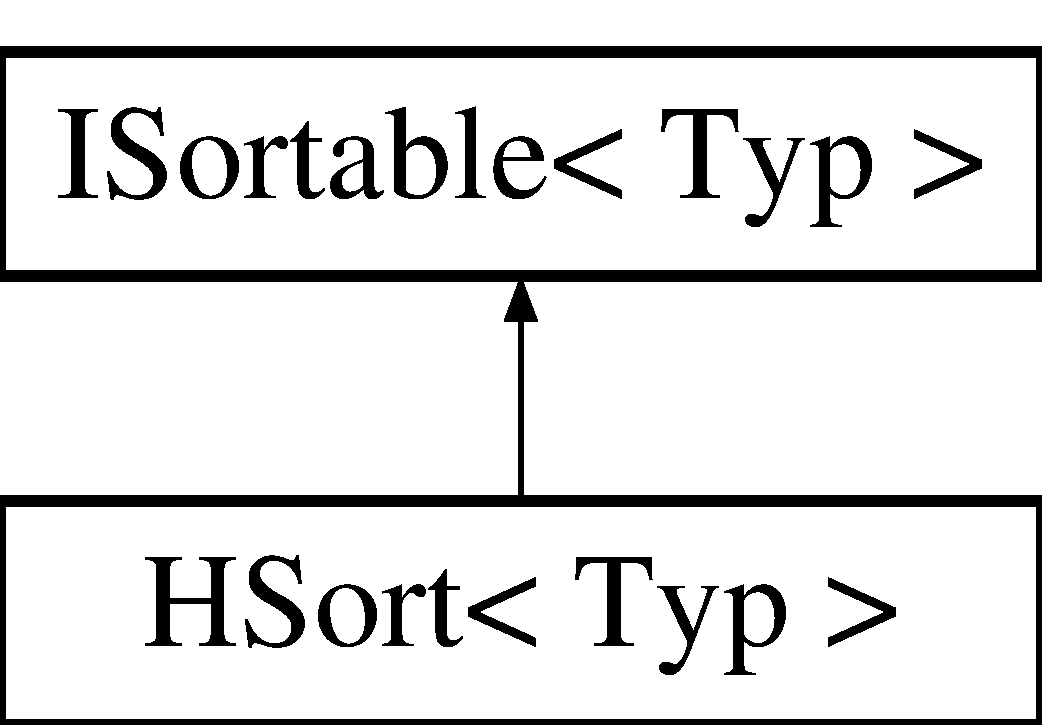
\includegraphics[height=2.000000cm]{class_h_sort}
\end{center}
\end{figure}
\subsection*{Public Member Functions}
\begin{DoxyCompactItemize}
\item 
void \hyperlink{class_h_sort_a02c33b82d229214ebd19787b7c9ead2d}{\-\_\-\-Sort} (\hyperlink{class_iterable}{Iterable}$<$ Typ $>$ $\ast$Kontener)
\begin{DoxyCompactList}\small\item\em Metoda inicjalizujaca sortowanie przez kopcowanie. \end{DoxyCompactList}\end{DoxyCompactItemize}
\subsection*{Private Member Functions}
\begin{DoxyCompactItemize}
\item 
void \hyperlink{class_h_sort_a1b59bf69e07408aa29281c3bb09da883}{Sortowanie\-Kopiec} (int Rozmiar, \hyperlink{class_iterable}{Iterable}$<$ Typ $>$ $\ast$K)
\begin{DoxyCompactList}\small\item\em Metoda sortowania przez Kopcowanie. \end{DoxyCompactList}\item 
void \hyperlink{class_h_sort_a062c4a39d5f9afa05ea07ff846a720e7}{Kopiec} (int Rozmiar, const int i, \hyperlink{class_iterable}{Iterable}$<$ Typ $>$ $\ast$K)
\begin{DoxyCompactList}\small\item\em Metoda skladajaca kopiec. \end{DoxyCompactList}\item 
void \hyperlink{class_h_sort_afba35e9a48f3d856b5fd090e8e44b372}{Buduj\-Kopiec} (int Rozmiar, \hyperlink{class_iterable}{Iterable}$<$ Typ $>$ $\ast$K)
\begin{DoxyCompactList}\small\item\em Metoda tworzaca kopiec. \end{DoxyCompactList}\end{DoxyCompactItemize}


\subsection{Detailed Description}
\subsubsection*{template$<$class Typ$>$class H\-Sort$<$ Typ $>$}

Modeluje sortowanie przez kopcowanie. 

Klasa zawiera implementacje algorytmu sortowania przez kopcowanie 

\subsection{Member Function Documentation}
\hypertarget{class_h_sort_a02c33b82d229214ebd19787b7c9ead2d}{\index{H\-Sort@{H\-Sort}!\-\_\-\-Sort@{\-\_\-\-Sort}}
\index{\-\_\-\-Sort@{\-\_\-\-Sort}!HSort@{H\-Sort}}
\subsubsection[{\-\_\-\-Sort}]{\setlength{\rightskip}{0pt plus 5cm}template$<$class Typ $>$ void {\bf H\-Sort}$<$ Typ $>$\-::\-\_\-\-Sort (
\begin{DoxyParamCaption}
\item[{{\bf Iterable}$<$ Typ $>$ $\ast$}]{Kontener}
\end{DoxyParamCaption}
)\hspace{0.3cm}{\ttfamily [inline]}, {\ttfamily [virtual]}}}\label{class_h_sort_a02c33b82d229214ebd19787b7c9ead2d}


Metoda inicjalizujaca sortowanie przez kopcowanie. 

Metoda ma za zadanie zainicjalizowac algorytm sortowania przez kopcowania dla wybranej struktury danych


\begin{DoxyParams}[1]{Parameters}
\mbox{\tt in}  & {\em Kontener} & -\/ rodzaj kontenera,ktory zostanie posortowany \\
\hline
\end{DoxyParams}


Implements \hyperlink{class_i_sortable_aca218e19355fb5d0e6ac7b29ea17dc59}{I\-Sortable$<$ Typ $>$}.

\hypertarget{class_h_sort_afba35e9a48f3d856b5fd090e8e44b372}{\index{H\-Sort@{H\-Sort}!Buduj\-Kopiec@{Buduj\-Kopiec}}
\index{Buduj\-Kopiec@{Buduj\-Kopiec}!HSort@{H\-Sort}}
\subsubsection[{Buduj\-Kopiec}]{\setlength{\rightskip}{0pt plus 5cm}template$<$class Typ $>$ void {\bf H\-Sort}$<$ Typ $>$\-::Buduj\-Kopiec (
\begin{DoxyParamCaption}
\item[{int}]{Rozmiar, }
\item[{{\bf Iterable}$<$ Typ $>$ $\ast$}]{K}
\end{DoxyParamCaption}
)\hspace{0.3cm}{\ttfamily [inline]}, {\ttfamily [private]}}}\label{class_h_sort_afba35e9a48f3d856b5fd090e8e44b372}


Metoda tworzaca kopiec. 

Metoda ma za zadanie utworzyc abstrakycjny kopiec z tablicy o podanym poprzez argument rozmiarze


\begin{DoxyParams}[1]{Parameters}
\mbox{\tt in}  & {\em Rozmiar} & -\/ Rozmiar kopca \\
\hline
\end{DoxyParams}
\hypertarget{class_h_sort_a062c4a39d5f9afa05ea07ff846a720e7}{\index{H\-Sort@{H\-Sort}!Kopiec@{Kopiec}}
\index{Kopiec@{Kopiec}!HSort@{H\-Sort}}
\subsubsection[{Kopiec}]{\setlength{\rightskip}{0pt plus 5cm}template$<$class Typ $>$ void {\bf H\-Sort}$<$ Typ $>$\-::Kopiec (
\begin{DoxyParamCaption}
\item[{int}]{Rozmiar, }
\item[{const int}]{i, }
\item[{{\bf Iterable}$<$ Typ $>$ $\ast$}]{K}
\end{DoxyParamCaption}
)\hspace{0.3cm}{\ttfamily [inline]}, {\ttfamily [private]}}}\label{class_h_sort_a062c4a39d5f9afa05ea07ff846a720e7}


Metoda skladajaca kopiec. 

Metoda ma za zadanie poprze porownywanie i ustawianie elementow odtworzenie porzadku kopcowego.


\begin{DoxyParams}[1]{Parameters}
\mbox{\tt in}  & {\em Rozmiar} & -\/ Rozmar kopca \\
\hline
\mbox{\tt in}  & {\em i} & -\/ indeks ostatniego elementu podzbioru \\
\hline
\end{DoxyParams}
\hypertarget{class_h_sort_a1b59bf69e07408aa29281c3bb09da883}{\index{H\-Sort@{H\-Sort}!Sortowanie\-Kopiec@{Sortowanie\-Kopiec}}
\index{Sortowanie\-Kopiec@{Sortowanie\-Kopiec}!HSort@{H\-Sort}}
\subsubsection[{Sortowanie\-Kopiec}]{\setlength{\rightskip}{0pt plus 5cm}template$<$class Typ $>$ void {\bf H\-Sort}$<$ Typ $>$\-::Sortowanie\-Kopiec (
\begin{DoxyParamCaption}
\item[{int}]{Rozmiar, }
\item[{{\bf Iterable}$<$ Typ $>$ $\ast$}]{K}
\end{DoxyParamCaption}
)\hspace{0.3cm}{\ttfamily [inline]}, {\ttfamily [private]}}}\label{class_h_sort_a1b59bf69e07408aa29281c3bb09da883}


Metoda sortowania przez Kopcowanie. 

Metoda realizujaca sortowanie rosnace,wykorzystujac przy tym kopiec.


\begin{DoxyParams}[1]{Parameters}
\mbox{\tt in}  & {\em Rozmiar} & -\/ Rozmiar kopca do zbudowania, ilość danych do posortowania. \\
\hline
\end{DoxyParams}


The documentation for this class was generated from the following file\-:\begin{DoxyCompactItemize}
\item 
/home/bartolomeo/209296/prj/inc/\hyperlink{_h_sort_8hh}{H\-Sort.\-hh}\end{DoxyCompactItemize}

\hypertarget{class_hyb_sort}{\section{Hyb\-Sort$<$ Typ $>$ Class Template Reference}
\label{class_hyb_sort}\index{Hyb\-Sort$<$ Typ $>$@{Hyb\-Sort$<$ Typ $>$}}
}


Modeluje sortowania hybrydowego.  




{\ttfamily \#include $<$Hyb\-Sort.\-hh$>$}

Inheritance diagram for Hyb\-Sort$<$ Typ $>$\-:\begin{figure}[H]
\begin{center}
\leavevmode
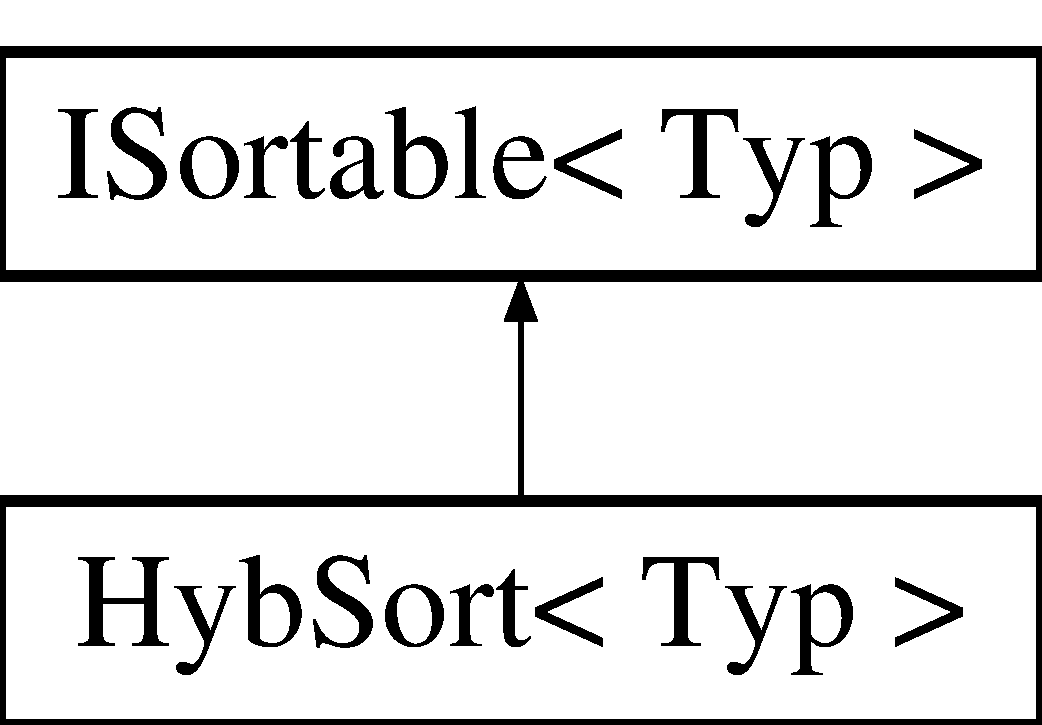
\includegraphics[height=2.000000cm]{class_hyb_sort}
\end{center}
\end{figure}
\subsection*{Public Member Functions}
\begin{DoxyCompactItemize}
\item 
void \hyperlink{class_hyb_sort_af12772bd67fad3bed145474a48b4c8b3}{\-\_\-\-Sort} (\hyperlink{class_iterable}{Iterable}$<$ Typ $>$ $\ast$Kontener)
\begin{DoxyCompactList}\small\item\em Metoda inicjalizujaca sortowanie hybrydowe. \end{DoxyCompactList}\end{DoxyCompactItemize}
\subsection*{Private Member Functions}
\begin{DoxyCompactItemize}
\item 
int \hyperlink{class_hyb_sort_a3a202fcd27870bb2b56bb256586cacdc}{Mediana} (Typ $\ast$W) const 
\begin{DoxyCompactList}\small\item\em Mediana Metoda wyznaczajaca mediana dla tablicy 3 elementowej. Jest to metoda pomocnicza, wykorzystywana przy optymalizacji doboru pivotu w sortowaniu szybkim. \end{DoxyCompactList}\item 
int \hyperlink{class_hyb_sort_ac6196e148240080a240ca990c7f740bb}{Partycjowanie} (int p, int k, \hyperlink{class_iterable}{Iterable}$<$ Typ $>$ $\ast$K)
\begin{DoxyCompactList}\small\item\em Zotymalizowane Sortowanie Szybkie. \end{DoxyCompactList}\item 
void \hyperlink{class_hyb_sort_afdf20a6c2fc2101bf9b1851919f910b7}{Wstaw\-\_\-\-Sort} (int l, int p, \hyperlink{class_iterable}{Iterable}$<$ Typ $>$ $\ast$K)
\begin{DoxyCompactList}\small\item\em Sortowanie przez Wstawianie Metoda ma za zadanie posortowac tablice przyjmowana jako argument. \end{DoxyCompactList}\item 
void \hyperlink{class_hyb_sort_aafe7b17d8af23857d648f8f35a281809}{Sortowanie\-\_\-\-Hybrydowe} (int l, int h, \hyperlink{class_iterable}{Iterable}$<$ Typ $>$ $\ast$K)
\begin{DoxyCompactList}\small\item\em Metoda sortowania hybrydowego. \end{DoxyCompactList}\end{DoxyCompactItemize}


\subsection{Detailed Description}
\subsubsection*{template$<$class Typ$>$class Hyb\-Sort$<$ Typ $>$}

Modeluje sortowania hybrydowego. 

Klasa zawiera implementacje algorytmu sortowania hybrydowego 

\subsection{Member Function Documentation}
\hypertarget{class_hyb_sort_af12772bd67fad3bed145474a48b4c8b3}{\index{Hyb\-Sort@{Hyb\-Sort}!\-\_\-\-Sort@{\-\_\-\-Sort}}
\index{\-\_\-\-Sort@{\-\_\-\-Sort}!HybSort@{Hyb\-Sort}}
\subsubsection[{\-\_\-\-Sort}]{\setlength{\rightskip}{0pt plus 5cm}template$<$class Typ $>$ void {\bf Hyb\-Sort}$<$ Typ $>$\-::\-\_\-\-Sort (
\begin{DoxyParamCaption}
\item[{{\bf Iterable}$<$ Typ $>$ $\ast$}]{Kontener}
\end{DoxyParamCaption}
)\hspace{0.3cm}{\ttfamily [inline]}, {\ttfamily [virtual]}}}\label{class_hyb_sort_af12772bd67fad3bed145474a48b4c8b3}


Metoda inicjalizujaca sortowanie hybrydowe. 

Metoda ma za zadanie zainicjalizowac algorytm sortowania hybrydowego dla wybranej struktury danych


\begin{DoxyParams}[1]{Parameters}
\mbox{\tt in}  & {\em Kontener} & -\/ rodzaj kontenera,ktory zostanie posortowany \\
\hline
\end{DoxyParams}


Implements \hyperlink{class_i_sortable_aca218e19355fb5d0e6ac7b29ea17dc59}{I\-Sortable$<$ Typ $>$}.

\hypertarget{class_hyb_sort_a3a202fcd27870bb2b56bb256586cacdc}{\index{Hyb\-Sort@{Hyb\-Sort}!Mediana@{Mediana}}
\index{Mediana@{Mediana}!HybSort@{Hyb\-Sort}}
\subsubsection[{Mediana}]{\setlength{\rightskip}{0pt plus 5cm}template$<$class Typ $>$ int {\bf Hyb\-Sort}$<$ Typ $>$\-::Mediana (
\begin{DoxyParamCaption}
\item[{Typ $\ast$}]{W}
\end{DoxyParamCaption}
) const\hspace{0.3cm}{\ttfamily [inline]}, {\ttfamily [private]}}}\label{class_hyb_sort_a3a202fcd27870bb2b56bb256586cacdc}


Mediana Metoda wyznaczajaca mediana dla tablicy 3 elementowej. Jest to metoda pomocnicza, wykorzystywana przy optymalizacji doboru pivotu w sortowaniu szybkim. 

\begin{DoxyReturn}{Returns}
Zwraca indeks na ktorym znajduje sie mediana w tablicy wejsciowej 
\end{DoxyReturn}
\hypertarget{class_hyb_sort_ac6196e148240080a240ca990c7f740bb}{\index{Hyb\-Sort@{Hyb\-Sort}!Partycjowanie@{Partycjowanie}}
\index{Partycjowanie@{Partycjowanie}!HybSort@{Hyb\-Sort}}
\subsubsection[{Partycjowanie}]{\setlength{\rightskip}{0pt plus 5cm}template$<$class Typ $>$ int {\bf Hyb\-Sort}$<$ Typ $>$\-::Partycjowanie (
\begin{DoxyParamCaption}
\item[{int}]{p, }
\item[{int}]{k, }
\item[{{\bf Iterable}$<$ Typ $>$ $\ast$}]{K}
\end{DoxyParamCaption}
)\hspace{0.3cm}{\ttfamily [inline]}, {\ttfamily [private]}}}\label{class_hyb_sort_ac6196e148240080a240ca990c7f740bb}


Zotymalizowane Sortowanie Szybkie. 

Metoda modeluje algorytm sorotwanie szybkiego z zaimplementowanym algorytmem doboru pivotu, tak aby nie zostal wybrany najmniejszy element w danym podzbiorze.

\mbox{[}in\mbox{]} lewy -\/ poczatkowy indeks pozbioru 
\begin{DoxyParams}[1]{Parameters}
\mbox{\tt in}  & {\em prawy} & -\/ koncowy indeks podzbioru \\
\hline
\end{DoxyParams}
\hypertarget{class_hyb_sort_aafe7b17d8af23857d648f8f35a281809}{\index{Hyb\-Sort@{Hyb\-Sort}!Sortowanie\-\_\-\-Hybrydowe@{Sortowanie\-\_\-\-Hybrydowe}}
\index{Sortowanie\-\_\-\-Hybrydowe@{Sortowanie\-\_\-\-Hybrydowe}!HybSort@{Hyb\-Sort}}
\subsubsection[{Sortowanie\-\_\-\-Hybrydowe}]{\setlength{\rightskip}{0pt plus 5cm}template$<$class Typ $>$ void {\bf Hyb\-Sort}$<$ Typ $>$\-::Sortowanie\-\_\-\-Hybrydowe (
\begin{DoxyParamCaption}
\item[{int}]{l, }
\item[{int}]{h, }
\item[{{\bf Iterable}$<$ Typ $>$ $\ast$}]{K}
\end{DoxyParamCaption}
)\hspace{0.3cm}{\ttfamily [inline]}, {\ttfamily [private]}}}\label{class_hyb_sort_aafe7b17d8af23857d648f8f35a281809}


Metoda sortowania hybrydowego. 

Metoda ta jest implementacja algorytmu sortowania hybrydowego, bedacego polaczeniem sortowania szybkiego i sortowania przez wstawianie Po zakonczeniu rekurencyjnych wywolan Partycjowania, tablica jest podzielona na szereg malych podzbiorow o o rozmiarze nie przekraczajacemu ustalonego progu. Zbioru sa porozdzielana elementami ktore wykorzystywane byly jako elementy osiowe. Dla czesciowo posortowanej tablicy wywolywane jest sortowanie przez wstawianie, ktore jest wydajne dla tablic o malych rozmiarach


\begin{DoxyParams}[1]{Parameters}
\mbox{\tt in}  & {\em l} & -\/ indeks poczatkowego elementu pozbioru \\
\hline
\mbox{\tt in}  & {\em h} & -\/ indeks koncowego elementu podzbioru \\
\hline
\end{DoxyParams}
\hypertarget{class_hyb_sort_afdf20a6c2fc2101bf9b1851919f910b7}{\index{Hyb\-Sort@{Hyb\-Sort}!Wstaw\-\_\-\-Sort@{Wstaw\-\_\-\-Sort}}
\index{Wstaw\-\_\-\-Sort@{Wstaw\-\_\-\-Sort}!HybSort@{Hyb\-Sort}}
\subsubsection[{Wstaw\-\_\-\-Sort}]{\setlength{\rightskip}{0pt plus 5cm}template$<$class Typ $>$ void {\bf Hyb\-Sort}$<$ Typ $>$\-::Wstaw\-\_\-\-Sort (
\begin{DoxyParamCaption}
\item[{int}]{l, }
\item[{int}]{p, }
\item[{{\bf Iterable}$<$ Typ $>$ $\ast$}]{K}
\end{DoxyParamCaption}
)\hspace{0.3cm}{\ttfamily [inline]}, {\ttfamily [private]}}}\label{class_hyb_sort_afdf20a6c2fc2101bf9b1851919f910b7}


Sortowanie przez Wstawianie Metoda ma za zadanie posortowac tablice przyjmowana jako argument. 


\begin{DoxyParams}[1]{Parameters}
\mbox{\tt in}  & {\em T} & -\/ Wskaznik na tablice z danymi wejsciowymi \\
\hline
\mbox{\tt in}  & {\em l} & -\/ Poczatkowy indeks elementu sortowanego podzbioru \\
\hline
\mbox{\tt in}  & {\em p} & -\/ koncowy indeks elementu sortowanego podzbioru \\
\hline
\end{DoxyParams}


The documentation for this class was generated from the following file\-:\begin{DoxyCompactItemize}
\item 
/home/bartolomeo/209296/prj/inc/\hyperlink{_hyb_sort_8hh}{Hyb\-Sort.\-hh}\end{DoxyCompactItemize}

\hypertarget{class_i_obserwator}{\section{I\-Obserwator Class Reference}
\label{class_i_obserwator}\index{I\-Obserwator@{I\-Obserwator}}
}


Modeluje pojecie interfejsu dla obserwatora.  




{\ttfamily \#include $<$I\-Obserwator.\-hh$>$}

Inheritance diagram for I\-Obserwator\-:\begin{figure}[H]
\begin{center}
\leavevmode
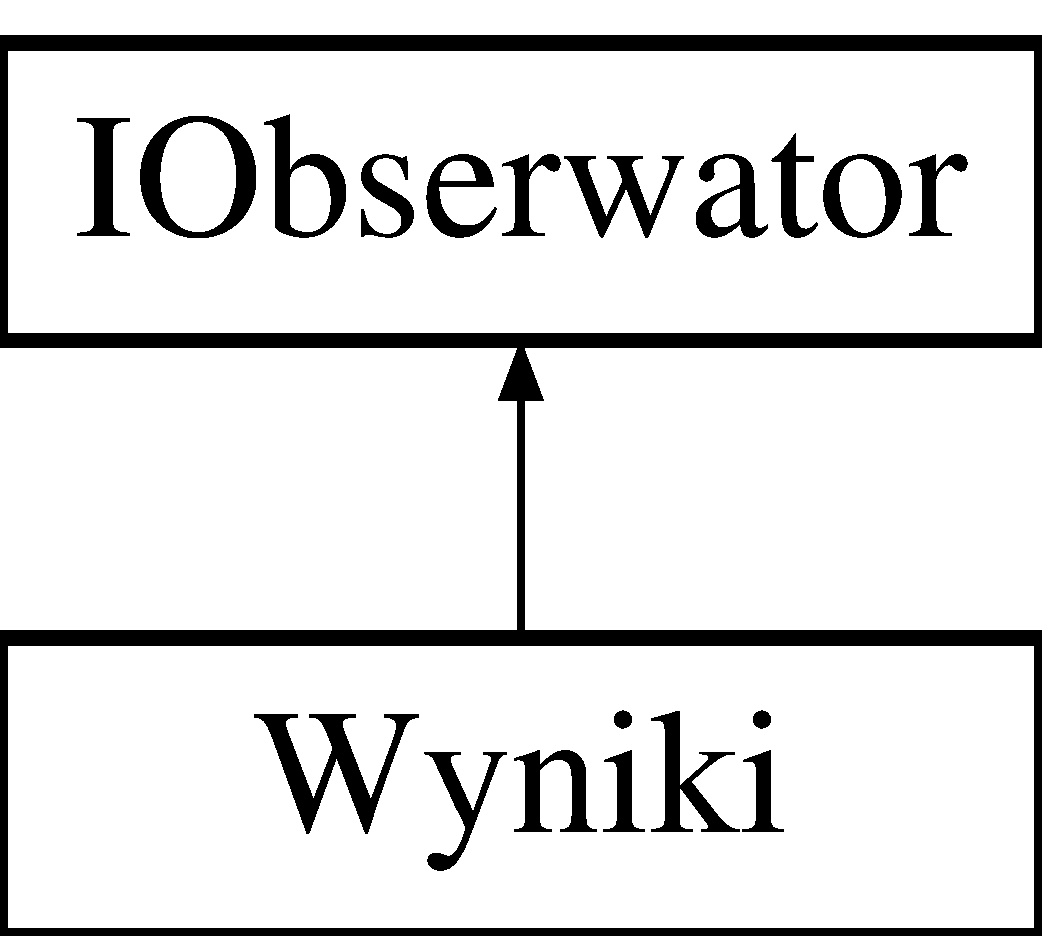
\includegraphics[height=2.000000cm]{class_i_obserwator}
\end{center}
\end{figure}
\subsection*{Public Member Functions}
\begin{DoxyCompactItemize}
\item 
virtual void \hyperlink{class_i_obserwator_ab01d64a94e127100951aa287d4d2275f}{\-\_\-\-Aktualizuj} ()=0
\begin{DoxyCompactList}\small\item\em Metoda Aktualizujaca stan. \end{DoxyCompactList}\end{DoxyCompactItemize}


\subsection{Detailed Description}
Modeluje pojecie interfejsu dla obserwatora. 

Klasa ta modeluje interfejs dla obiektu ktory bedzie obserwatorem 

\subsection{Member Function Documentation}
\hypertarget{class_i_obserwator_ab01d64a94e127100951aa287d4d2275f}{\index{I\-Obserwator@{I\-Obserwator}!\-\_\-\-Aktualizuj@{\-\_\-\-Aktualizuj}}
\index{\-\_\-\-Aktualizuj@{\-\_\-\-Aktualizuj}!IObserwator@{I\-Obserwator}}
\subsubsection[{\-\_\-\-Aktualizuj}]{\setlength{\rightskip}{0pt plus 5cm}virtual void I\-Obserwator\-::\-\_\-\-Aktualizuj (
\begin{DoxyParamCaption}
{}
\end{DoxyParamCaption}
)\hspace{0.3cm}{\ttfamily [pure virtual]}}}\label{class_i_obserwator_ab01d64a94e127100951aa287d4d2275f}


Metoda Aktualizujaca stan. 

Metoda ma za zadanie poinformowac o zmianach w obiekcie ktory jest obserwowany 

Implemented in \hyperlink{class_wyniki_a4014236438f62cfd90c03de49ea38e5f}{Wyniki}.



The documentation for this class was generated from the following file\-:\begin{DoxyCompactItemize}
\item 
/home/bartolomeo/209296/prj/inc/\hyperlink{_i_obserwator_8hh}{I\-Obserwator.\-hh}\end{DoxyCompactItemize}

\hypertarget{class_i_obserwowany}{\section{I\-Obserwowany Class Reference}
\label{class_i_obserwowany}\index{I\-Obserwowany@{I\-Obserwowany}}
}


Interfejs dla Obserwatora.  




{\ttfamily \#include $<$I\-Obserwowany.\-hh$>$}

Inheritance diagram for I\-Obserwowany\-:\begin{figure}[H]
\begin{center}
\leavevmode
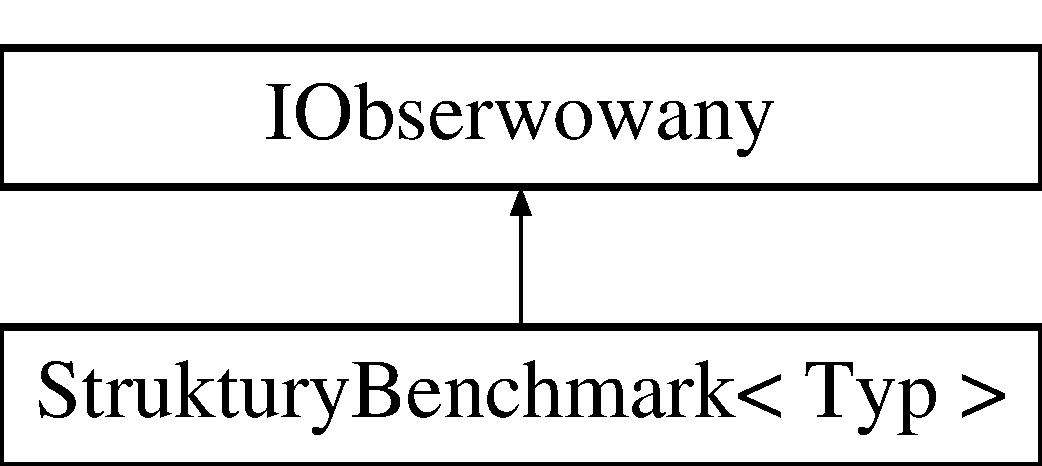
\includegraphics[height=2.000000cm]{class_i_obserwowany}
\end{center}
\end{figure}
\subsection*{Protected Member Functions}
\begin{DoxyCompactItemize}
\item 
virtual void \hyperlink{class_i_obserwowany_a3e7c49a1b168ed5a3f84bd0c5ae27513}{\-\_\-\-Dodaj\-Obserwator} (\hyperlink{class_i_obserwator}{I\-Obserwator} $\ast$O)=0
\begin{DoxyCompactList}\small\item\em Metoda dodajaca obserwator. \end{DoxyCompactList}\item 
virtual void \hyperlink{class_i_obserwowany_a6e91b84d0502f038d287152a5d860aff}{\-\_\-\-Usun\-Obserwator} (\hyperlink{class_i_obserwator}{I\-Obserwator} $\ast$O)=0
\begin{DoxyCompactList}\small\item\em Metoda usuwajaca obserwator. \end{DoxyCompactList}\item 
virtual void \hyperlink{class_i_obserwowany_addbe1bee0cae92b0c1348b2c6d0b525c}{\-\_\-\-Powiadom\-Obserwatorow} ()=0
\begin{DoxyCompactList}\small\item\em Metoda informujaca obserwatorow. \end{DoxyCompactList}\end{DoxyCompactItemize}


\subsection{Detailed Description}
Interfejs dla Obserwatora. 

Klasa modeluje pojecie abstrakcyjnego interfejsu dla klasy bedacej obiektem obserwowanym 

\subsection{Member Function Documentation}
\hypertarget{class_i_obserwowany_a3e7c49a1b168ed5a3f84bd0c5ae27513}{\index{I\-Obserwowany@{I\-Obserwowany}!\-\_\-\-Dodaj\-Obserwator@{\-\_\-\-Dodaj\-Obserwator}}
\index{\-\_\-\-Dodaj\-Obserwator@{\-\_\-\-Dodaj\-Obserwator}!IObserwowany@{I\-Obserwowany}}
\subsubsection[{\-\_\-\-Dodaj\-Obserwator}]{\setlength{\rightskip}{0pt plus 5cm}virtual void I\-Obserwowany\-::\-\_\-\-Dodaj\-Obserwator (
\begin{DoxyParamCaption}
\item[{{\bf I\-Obserwator} $\ast$}]{O}
\end{DoxyParamCaption}
)\hspace{0.3cm}{\ttfamily [protected]}, {\ttfamily [pure virtual]}}}\label{class_i_obserwowany_a3e7c49a1b168ed5a3f84bd0c5ae27513}


Metoda dodajaca obserwator. 

Metoda ma za zadanie dodac nowego obserwatora do listy obserwatorow danego obiektu


\begin{DoxyParams}[1]{Parameters}
\mbox{\tt in}  & {\em O} & -\/ wskaznik na dodawany obserwator \\
\hline
\end{DoxyParams}


Implemented in \hyperlink{class_struktury_benchmark_a63247cc5616565e429f5abd09d887630}{Struktury\-Benchmark$<$ Typ $>$}.

\hypertarget{class_i_obserwowany_addbe1bee0cae92b0c1348b2c6d0b525c}{\index{I\-Obserwowany@{I\-Obserwowany}!\-\_\-\-Powiadom\-Obserwatorow@{\-\_\-\-Powiadom\-Obserwatorow}}
\index{\-\_\-\-Powiadom\-Obserwatorow@{\-\_\-\-Powiadom\-Obserwatorow}!IObserwowany@{I\-Obserwowany}}
\subsubsection[{\-\_\-\-Powiadom\-Obserwatorow}]{\setlength{\rightskip}{0pt plus 5cm}virtual void I\-Obserwowany\-::\-\_\-\-Powiadom\-Obserwatorow (
\begin{DoxyParamCaption}
{}
\end{DoxyParamCaption}
)\hspace{0.3cm}{\ttfamily [protected]}, {\ttfamily [pure virtual]}}}\label{class_i_obserwowany_addbe1bee0cae92b0c1348b2c6d0b525c}


Metoda informujaca obserwatorow. 

Metoda ma za zadanie poinformowac wszystkich obserwatorow o zmianach, ktore sa istotne dla nich, jakie zostaly wykonane na obiekcie obserwowanym 

Implemented in \hyperlink{class_struktury_benchmark_af5aa09efcf9a1727e0868930b97ede49}{Struktury\-Benchmark$<$ Typ $>$}.

\hypertarget{class_i_obserwowany_a6e91b84d0502f038d287152a5d860aff}{\index{I\-Obserwowany@{I\-Obserwowany}!\-\_\-\-Usun\-Obserwator@{\-\_\-\-Usun\-Obserwator}}
\index{\-\_\-\-Usun\-Obserwator@{\-\_\-\-Usun\-Obserwator}!IObserwowany@{I\-Obserwowany}}
\subsubsection[{\-\_\-\-Usun\-Obserwator}]{\setlength{\rightskip}{0pt plus 5cm}virtual void I\-Obserwowany\-::\-\_\-\-Usun\-Obserwator (
\begin{DoxyParamCaption}
\item[{{\bf I\-Obserwator} $\ast$}]{O}
\end{DoxyParamCaption}
)\hspace{0.3cm}{\ttfamily [protected]}, {\ttfamily [pure virtual]}}}\label{class_i_obserwowany_a6e91b84d0502f038d287152a5d860aff}


Metoda usuwajaca obserwator. 

Metoda ma za zadanei usunac zadanego poprzez argument obserwatora z listy obserwatorow danego obiektu


\begin{DoxyParams}[1]{Parameters}
\mbox{\tt in}  & {\em O} & -\/ wskaznik na obserwator,ktory ma zostac usuniety \\
\hline
\end{DoxyParams}


Implemented in \hyperlink{class_struktury_benchmark_af08fe671ed7528428ffcb8a4daf65197}{Struktury\-Benchmark$<$ Typ $>$}.



The documentation for this class was generated from the following file\-:\begin{DoxyCompactItemize}
\item 
/home/bartolomeo/209296/prj/inc/\hyperlink{_i_obserwowany_8hh}{I\-Obserwowany.\-hh}\end{DoxyCompactItemize}

\hypertarget{class_i_sortable}{\section{I\-Sortable$<$ Typ $>$ Class Template Reference}
\label{class_i_sortable}\index{I\-Sortable$<$ Typ $>$@{I\-Sortable$<$ Typ $>$}}
}


Definicja klasy \hyperlink{class_i_sortable}{I\-Sortable}.  




{\ttfamily \#include $<$I\-Sortable.\-hh$>$}

Inheritance diagram for I\-Sortable$<$ Typ $>$\-:\begin{figure}[H]
\begin{center}
\leavevmode
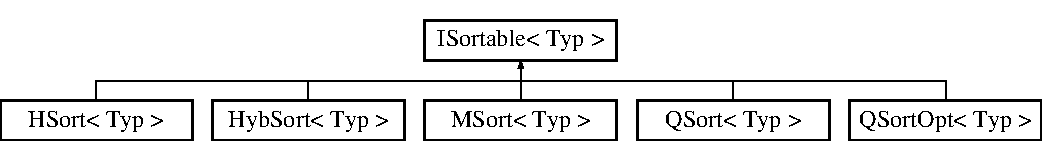
\includegraphics[height=1.898305cm]{class_i_sortable}
\end{center}
\end{figure}
\subsection*{Public Member Functions}
\begin{DoxyCompactItemize}
\item 
virtual void \hyperlink{class_i_sortable_aca218e19355fb5d0e6ac7b29ea17dc59}{\-\_\-\-Sort} (\hyperlink{class_iterable}{Iterable}$<$ Typ $>$ $\ast$Kontener)=0
\begin{DoxyCompactList}\small\item\em Metoda inicjalizujaca sortowanie. \end{DoxyCompactList}\end{DoxyCompactItemize}


\subsection{Detailed Description}
\subsubsection*{template$<$class Typ$>$class I\-Sortable$<$ Typ $>$}

Definicja klasy \hyperlink{class_i_sortable}{I\-Sortable}. 

Klasa modeluje pojecie abstrakcyjnego interfejsu \hyperlink{class_i_sortable}{I\-Sortable}, dzieki ktoremu uzytkownik moze wykorzystac dowolny algorytm sortowania dla wybranego konteneru 

\subsection{Member Function Documentation}
\hypertarget{class_i_sortable_aca218e19355fb5d0e6ac7b29ea17dc59}{\index{I\-Sortable@{I\-Sortable}!\-\_\-\-Sort@{\-\_\-\-Sort}}
\index{\-\_\-\-Sort@{\-\_\-\-Sort}!ISortable@{I\-Sortable}}
\subsubsection[{\-\_\-\-Sort}]{\setlength{\rightskip}{0pt plus 5cm}template$<$class Typ$>$ virtual void {\bf I\-Sortable}$<$ Typ $>$\-::\-\_\-\-Sort (
\begin{DoxyParamCaption}
\item[{{\bf Iterable}$<$ Typ $>$ $\ast$}]{Kontener}
\end{DoxyParamCaption}
)\hspace{0.3cm}{\ttfamily [pure virtual]}}}\label{class_i_sortable_aca218e19355fb5d0e6ac7b29ea17dc59}


Metoda inicjalizujaca sortowanie. 

Metoda ma za zadanie uruchomic dowolny zaimplementowany algorytm sortowania dla struktury danych okreslonej poprzez argument jaki przyjmuje ta metoda


\begin{DoxyParams}[1]{Parameters}
\mbox{\tt in}  & {\em Kontener} & -\/ wskaznik na obiekt ktory ma ulec posortowaniu \\
\hline
\end{DoxyParams}


Implemented in \hyperlink{class_hyb_sort_af12772bd67fad3bed145474a48b4c8b3}{Hyb\-Sort$<$ Typ $>$}, \hyperlink{class_q_sort_opt_af9283edf949f7631c4f08f4b945370fa}{Q\-Sort\-Opt$<$ Typ $>$}, \hyperlink{class_h_sort_a02c33b82d229214ebd19787b7c9ead2d}{H\-Sort$<$ Typ $>$}, \hyperlink{class_m_sort_a90bfe37f7a17b529b97abba47495ab9a}{M\-Sort$<$ Typ $>$}, and \hyperlink{class_q_sort_a059dc69db4a44032648c766e20c92126}{Q\-Sort$<$ Typ $>$}.



The documentation for this class was generated from the following file\-:\begin{DoxyCompactItemize}
\item 
/home/bartolomeo/209296/prj/inc/\hyperlink{_i_sortable_8hh}{I\-Sortable.\-hh}\end{DoxyCompactItemize}

\hypertarget{class_iterable}{\section{Iterable$<$ Typ $>$ Class Template Reference}
\label{class_iterable}\index{Iterable$<$ Typ $>$@{Iterable$<$ Typ $>$}}
}


Interfejs \hyperlink{class_iterable}{Iterable}.  




{\ttfamily \#include $<$Iterable.\-hh$>$}

Inheritance diagram for Iterable$<$ Typ $>$\-:\begin{figure}[H]
\begin{center}
\leavevmode
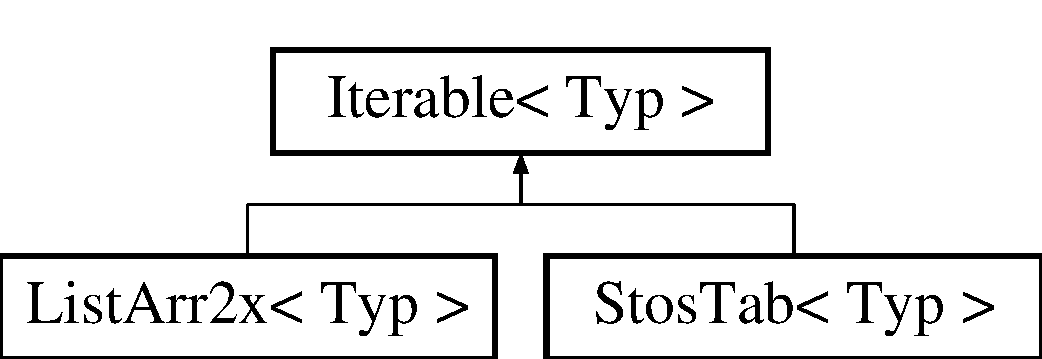
\includegraphics[height=2.000000cm]{class_iterable}
\end{center}
\end{figure}
\subsection*{Public Member Functions}
\begin{DoxyCompactItemize}
\item 
virtual const Typ \hyperlink{class_iterable_a6b75a7c8c41e1f13e6eff2276af62aeb}{Wartosc} (unsigned int i) const =0
\begin{DoxyCompactList}\small\item\em Metoda zwracajaca wartosc. \end{DoxyCompactList}\item 
virtual Typ \& \hyperlink{class_iterable_a7e56512db9ef2691198e1914a4ddb300}{Adres} (unsigned int i)=0
\begin{DoxyCompactList}\small\item\em Metoda zwracajaca referencje. \end{DoxyCompactList}\item 
virtual void \hyperlink{class_iterable_a631b741c6f81ae09f823c86f9eed9f7b}{\-\_\-\-Zamien} (unsigned int i, unsigned int j)=0
\begin{DoxyCompactList}\small\item\em Metoda zamieniajaca. \end{DoxyCompactList}\item 
virtual unsigned int \hyperlink{class_iterable_ab5962acaeaa36a245b18a7c66fac972f}{\-\_\-\-Rozmiar} () const =0
\begin{DoxyCompactList}\small\item\em Metoda informujaca o rozmiarze. \end{DoxyCompactList}\end{DoxyCompactItemize}


\subsection{Detailed Description}
\subsubsection*{template$<$class Typ$>$class Iterable$<$ Typ $>$}

Interfejs \hyperlink{class_iterable}{Iterable}. 

Klasa modeluje pojecie abstrakcyjnego interfejsu iterable, dzieki ktoremu algorytmu sortujace maja dostep do kontenera z danymi poprzez odczyt danego pola i mozliwosci zamiany elementow miejscami 

\subsection{Member Function Documentation}
\hypertarget{class_iterable_ab5962acaeaa36a245b18a7c66fac972f}{\index{Iterable@{Iterable}!\-\_\-\-Rozmiar@{\-\_\-\-Rozmiar}}
\index{\-\_\-\-Rozmiar@{\-\_\-\-Rozmiar}!Iterable@{Iterable}}
\subsubsection[{\-\_\-\-Rozmiar}]{\setlength{\rightskip}{0pt plus 5cm}template$<$class Typ$>$ virtual unsigned int {\bf Iterable}$<$ Typ $>$\-::\-\_\-\-Rozmiar (
\begin{DoxyParamCaption}
{}
\end{DoxyParamCaption}
) const\hspace{0.3cm}{\ttfamily [pure virtual]}}}\label{class_iterable_ab5962acaeaa36a245b18a7c66fac972f}


Metoda informujaca o rozmiarze. 

Metoda ma za zadanie zwrocic informajce o rozmiarze kontenera 

Implemented in \hyperlink{class_list_arr2x_aa9d38356df7fec58f282ec00148bd6db}{List\-Arr2x$<$ Typ $>$}, and \hyperlink{class_stos_tab_a51b2da61d6c4c2085646b84395c2d3c0}{Stos\-Tab$<$ Typ $>$}.

\hypertarget{class_iterable_a631b741c6f81ae09f823c86f9eed9f7b}{\index{Iterable@{Iterable}!\-\_\-\-Zamien@{\-\_\-\-Zamien}}
\index{\-\_\-\-Zamien@{\-\_\-\-Zamien}!Iterable@{Iterable}}
\subsubsection[{\-\_\-\-Zamien}]{\setlength{\rightskip}{0pt plus 5cm}template$<$class Typ$>$ virtual void {\bf Iterable}$<$ Typ $>$\-::\-\_\-\-Zamien (
\begin{DoxyParamCaption}
\item[{unsigned int}]{i, }
\item[{unsigned int}]{j}
\end{DoxyParamCaption}
)\hspace{0.3cm}{\ttfamily [pure virtual]}}}\label{class_iterable_a631b741c6f81ae09f823c86f9eed9f7b}


Metoda zamieniajaca. 

Metoda ma za zadanie zamienic elementy miejscami 
\begin{DoxyParams}[1]{Parameters}
\mbox{\tt in}  & {\em i} & -\/ indeks,pod ktorym wartosc z konteneru zostanie zamieniona miejscem \\
\hline
\mbox{\tt in}  & {\em j} & -\/ indeks,pod ktorym wartosc z konteneru zostanie zamieniona miejscem \\
\hline
\end{DoxyParams}


Implemented in \hyperlink{class_stos_tab_a6ce0e7f4dabae776f69fb0540ff7d8a4}{Stos\-Tab$<$ Typ $>$}, and \hyperlink{class_list_arr2x_a5864b6c097b593e0c126a79837f8fb19}{List\-Arr2x$<$ Typ $>$}.

\hypertarget{class_iterable_a7e56512db9ef2691198e1914a4ddb300}{\index{Iterable@{Iterable}!Adres@{Adres}}
\index{Adres@{Adres}!Iterable@{Iterable}}
\subsubsection[{Adres}]{\setlength{\rightskip}{0pt plus 5cm}template$<$class Typ$>$ virtual Typ\& {\bf Iterable}$<$ Typ $>$\-::Adres (
\begin{DoxyParamCaption}
\item[{unsigned int}]{i}
\end{DoxyParamCaption}
)\hspace{0.3cm}{\ttfamily [pure virtual]}}}\label{class_iterable_a7e56512db9ef2691198e1914a4ddb300}


Metoda zwracajaca referencje. 

Metoda ma za zadanie zwrocic referencje do pola kontenera zadanego poprzez argument metody 

Implemented in \hyperlink{class_list_arr2x_a18b7381c3fff0f489bd21dca90870f6f}{List\-Arr2x$<$ Typ $>$}, and \hyperlink{class_stos_tab_ad19a954bb9cc9c32b42e4046c422984a}{Stos\-Tab$<$ Typ $>$}.

\hypertarget{class_iterable_a6b75a7c8c41e1f13e6eff2276af62aeb}{\index{Iterable@{Iterable}!Wartosc@{Wartosc}}
\index{Wartosc@{Wartosc}!Iterable@{Iterable}}
\subsubsection[{Wartosc}]{\setlength{\rightskip}{0pt plus 5cm}template$<$class Typ$>$ virtual const Typ {\bf Iterable}$<$ Typ $>$\-::Wartosc (
\begin{DoxyParamCaption}
\item[{unsigned int}]{i}
\end{DoxyParamCaption}
) const\hspace{0.3cm}{\ttfamily [pure virtual]}}}\label{class_iterable_a6b75a7c8c41e1f13e6eff2276af62aeb}


Metoda zwracajaca wartosc. 

Metoda ma za zadanei zwrocic wartosc,kryjaca sie pod danym indeksem dla dowolnego kontenera posiadajacego interfejs.


\begin{DoxyParams}[1]{Parameters}
\mbox{\tt in}  & {\em i} & -\/\-Indeks z ktorego zostanie odczytana wartosc\\
\hline
\end{DoxyParams}
\begin{DoxyReturn}{Returns}
Zwraca wartosc, kryjaca sie pod danym indeksem konteneru 
\end{DoxyReturn}


Implemented in \hyperlink{class_list_arr2x_a1d441a5e86d979c8093543218faa13b3}{List\-Arr2x$<$ Typ $>$}, and \hyperlink{class_stos_tab_aeae02936cdfdb3df20084174817b85dd}{Stos\-Tab$<$ Typ $>$}.



The documentation for this class was generated from the following file\-:\begin{DoxyCompactItemize}
\item 
/home/bartolomeo/209296/prj/inc/\hyperlink{_iterable_8hh}{Iterable.\-hh}\end{DoxyCompactItemize}

\hypertarget{class_list_arr2x}{\subsection{List\-Arr2x$<$ typ $>$ Class Template Reference}
\label{class_list_arr2x}\index{List\-Arr2x$<$ typ $>$@{List\-Arr2x$<$ typ $>$}}
}


Modeluje pojęcie Listy (array)  




{\ttfamily \#include $<$List\-Arr2x.\-hh$>$}

Inheritance diagram for List\-Arr2x$<$ typ $>$\-:\begin{figure}[H]
\begin{center}
\leavevmode
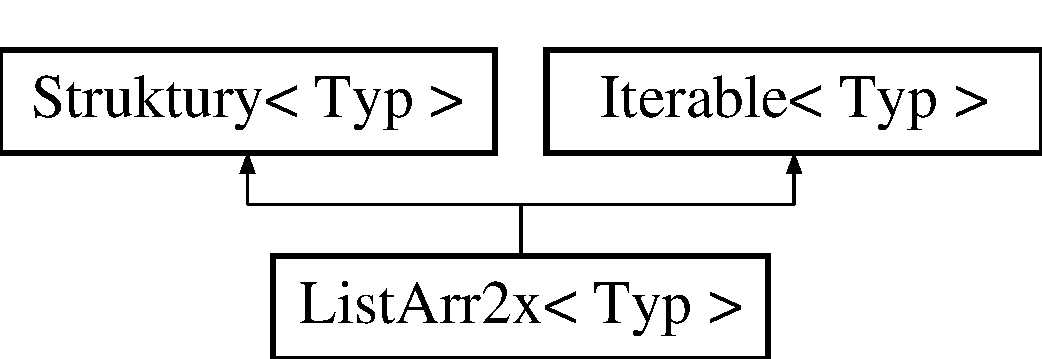
\includegraphics[height=3.000000cm]{class_list_arr2x}
\end{center}
\end{figure}
\subsubsection*{Public Member Functions}
\begin{DoxyCompactItemize}
\item 
\hyperlink{class_list_arr2x_abcda8405dca802e050c32cadb56f2caf}{List\-Arr2x} ()
\begin{DoxyCompactList}\small\item\em Konstruktor bezarumentowy. \end{DoxyCompactList}\item 
void \hyperlink{class_list_arr2x_a6aa004e56bdaf72de719d682b4069011}{push} (typ dana, unsigned int pole)
\begin{DoxyCompactList}\small\item\em Dodaje element do Listy\-Arr1. \end{DoxyCompactList}\item 
typ \hyperlink{class_list_arr2x_a6462ac1f547b7a090e54629539ce2dda}{pop} (unsigned int pole)
\begin{DoxyCompactList}\small\item\em Pobiera element z Listy\-Arr1. \end{DoxyCompactList}\item 
unsigned int \hyperlink{class_list_arr2x_a6097d85211e74053506d4a5dce86f26c}{size} ()
\begin{DoxyCompactList}\small\item\em Wielkość listy. \end{DoxyCompactList}\item 
void \hyperlink{class_list_arr2x_afd6469fa733da21b70981fa4dfae9c12}{Wczytaj\-Dane} (const std\-::string Plik\-In, unsigned int n)
\begin{DoxyCompactList}\small\item\em Wczytuje dane z pliku. \end{DoxyCompactList}\item 
void \hyperlink{class_list_arr2x_a7145b66ae33801053dc15bad1baa3085}{Qsort} (int l, int h)
\begin{DoxyCompactList}\small\item\em Metoda wykorzystujaca sortowanei szybkie. \end{DoxyCompactList}\item 
void \hyperlink{class_list_arr2x_a0c4ff2329317ccd77e48cf2965c80d91}{Qsort\-Opt} (int lewy, int prawy1)
\begin{DoxyCompactList}\small\item\em Zotymalizowane Sortowanie Szybkie. \end{DoxyCompactList}\item 
void \hyperlink{class_list_arr2x_a5f2644455c4c3a1ee9f1752a74857241}{Pokaz} ()
\begin{DoxyCompactList}\small\item\em Metoda wypisujaca elemeny listy. \end{DoxyCompactList}\item 
void \hyperlink{class_list_arr2x_a68dc47d3f73dbe42364bf34bdb132d00}{M\-Sort} (typ $\ast$T, int p, int k)
\end{DoxyCompactItemize}
\subsubsection*{Private Member Functions}
\begin{DoxyCompactItemize}
\item 
void \hyperlink{class_list_arr2x_abc4a5c934e4b30542f71045ec94c176b}{Wstaw\-\_\-\-Sort} (typ $\ast$T, int n)
\begin{DoxyCompactList}\small\item\em Sortowanie przez Wstawianie Metoda ma za zadanie posortowac tablice przyjmowana jako argument. \end{DoxyCompactList}\item 
int \hyperlink{class_list_arr2x_a8f0e72633b7bb63a37faaa99282b5308}{Mediana} (typ $\ast$W)
\begin{DoxyCompactList}\small\item\em Mediana Metoda wyznaczajaca mediana dla tablicy 3 elementowej. Jest to metoda pomocnicza, wykorzystywana przy optymalizacji doboru pivotu w sortowaniu szybkim. \end{DoxyCompactList}\item 
void \hyperlink{class_list_arr2x_adfd1dd69dadd19ac04ede03dba454fb5}{Start\-Msort} (unsigned int k)
\begin{DoxyCompactList}\small\item\em Metoda testująca czas. \end{DoxyCompactList}\item 
void \hyperlink{class_list_arr2x_ad73276a597d78b636119378ee408129d}{Start} ()
\begin{DoxyCompactList}\small\item\em Metoda testująca czas. \end{DoxyCompactList}\item 
void \hyperlink{class_list_arr2x_a8641af35d8316a58610a1c02ff4c3f83}{Zamien} (typ \&i, typ \&j)
\begin{DoxyCompactList}\small\item\em Metoda zamieniajaca Metoda ma za zadanie zamienic miejscami elementy wybrane przez argumenty wywolania. \end{DoxyCompactList}\item 
int \hyperlink{class_list_arr2x_a522da82666b97c2810ff458ef14e0996}{Partycjowanie} (int p, int k)
\begin{DoxyCompactList}\small\item\em Metoda segregujaca. \end{DoxyCompactList}\item 
void \hyperlink{class_list_arr2x_afcf6d8447657ff792afd631c54a4ff99}{Merge} (typ $\ast$Temp, int l, int s, int p)
\begin{DoxyCompactList}\small\item\em Metoda Dzielaca tablice. \end{DoxyCompactList}\item 
void \hyperlink{class_list_arr2x_a4e922603e7ed26334ee19cbca3c5056d}{Zwolnij} ()
\begin{DoxyCompactList}\small\item\em Zwalnia pamięć \end{DoxyCompactList}\end{DoxyCompactItemize}
\subsubsection*{Private Attributes}
\begin{DoxyCompactItemize}
\item 
typ $\ast$ \hyperlink{class_list_arr2x_aea5c139721e078af30bdc3c46cf58841}{tab}
\begin{DoxyCompactList}\small\item\em Wkaźnik na dynamiczną tablicę \end{DoxyCompactList}\item 
unsigned int \hyperlink{class_list_arr2x_aa25f050acca08e308c9b508f3ed8c912}{Rozmiar\-T}
\begin{DoxyCompactList}\small\item\em Rozmiar tablicy. \end{DoxyCompactList}\item 
unsigned int \hyperlink{class_list_arr2x_a17e0dfc0e9c86d433e0a79994af926c9}{Rozmiar\-L}
\begin{DoxyCompactList}\small\item\em Rozmiar Listy. \end{DoxyCompactList}\end{DoxyCompactItemize}


\subsubsection{Detailed Description}
\subsubsection*{template$<$class typ$>$class List\-Arr2x$<$ typ $>$}

Modeluje pojęcie Listy (array) 

Modeluje pojęcie Listy opartej na dynamicznej tablicy. Dodając elementy zwiększa tablicę dwukrotnie, jeżeli brakuje miejsca. 

Definition at line 23 of file List\-Arr2x.\-hh.



\subsubsection{Constructor \& Destructor Documentation}
\hypertarget{class_list_arr2x_abcda8405dca802e050c32cadb56f2caf}{\index{List\-Arr2x@{List\-Arr2x}!List\-Arr2x@{List\-Arr2x}}
\index{List\-Arr2x@{List\-Arr2x}!ListArr2x@{List\-Arr2x}}
\paragraph[{List\-Arr2x}]{\setlength{\rightskip}{0pt plus 5cm}template$<$class typ$>$ {\bf List\-Arr2x}$<$ typ $>$\-::{\bf List\-Arr2x} (
\begin{DoxyParamCaption}
{}
\end{DoxyParamCaption}
)\hspace{0.3cm}{\ttfamily [inline]}}}\label{class_list_arr2x_abcda8405dca802e050c32cadb56f2caf}


Konstruktor bezarumentowy. 

Kontruktor alokujący tablicę jednoelementową z której będzie tworzona lista 

Definition at line 222 of file List\-Arr2x.\-hh.



\subsubsection{Member Function Documentation}
\hypertarget{class_list_arr2x_a8f0e72633b7bb63a37faaa99282b5308}{\index{List\-Arr2x@{List\-Arr2x}!Mediana@{Mediana}}
\index{Mediana@{Mediana}!ListArr2x@{List\-Arr2x}}
\paragraph[{Mediana}]{\setlength{\rightskip}{0pt plus 5cm}template$<$class typ$>$ int {\bf List\-Arr2x}$<$ typ $>$\-::Mediana (
\begin{DoxyParamCaption}
\item[{typ $\ast$}]{W}
\end{DoxyParamCaption}
)\hspace{0.3cm}{\ttfamily [inline]}, {\ttfamily [private]}}}\label{class_list_arr2x_a8f0e72633b7bb63a37faaa99282b5308}


Mediana Metoda wyznaczajaca mediana dla tablicy 3 elementowej. Jest to metoda pomocnicza, wykorzystywana przy optymalizacji doboru pivotu w sortowaniu szybkim. 

\begin{DoxyReturn}{Returns}
Zwraca indeks na ktorym znajduje sie mediana w tablicy wejsciowej 
\end{DoxyReturn}


Definition at line 84 of file List\-Arr2x.\-hh.

\hypertarget{class_list_arr2x_afcf6d8447657ff792afd631c54a4ff99}{\index{List\-Arr2x@{List\-Arr2x}!Merge@{Merge}}
\index{Merge@{Merge}!ListArr2x@{List\-Arr2x}}
\paragraph[{Merge}]{\setlength{\rightskip}{0pt plus 5cm}template$<$class typ$>$ void {\bf List\-Arr2x}$<$ typ $>$\-::Merge (
\begin{DoxyParamCaption}
\item[{typ $\ast$}]{Temp, }
\item[{int}]{l, }
\item[{int}]{s, }
\item[{int}]{p}
\end{DoxyParamCaption}
)\hspace{0.3cm}{\ttfamily [inline]}, {\ttfamily [private]}}}\label{class_list_arr2x_afcf6d8447657ff792afd631c54a4ff99}


Metoda Dzielaca tablice. 

Metoda ma za zadanie przekopiowac zawartosc zbiotu glownego do tablicy tymczasowej.\-Nastepnie operujac na kopii ustawia wskazniki na poczatki kolejnych zbiorow i porownywane sa wskaane wartosci. Mniejsze wpisujemy do zbioru glownego i przesuwamy odpowiedni wskaznik Czynnos wykonujemy rekurencyjnie az do momentu gdy jeden ze wskaznikow osiagnie koniec zbioru


\begin{DoxyParams}[1]{Parameters}
\mbox{\tt in}  & {\em Temp} & -\/ Wskaznik na tablice pomocnicza \\
\hline
\mbox{\tt in}  & {\em l} & -\/ Poczatkowy indeks tablicy \\
\hline
\mbox{\tt in}  & {\em s} & -\/ Srodkowy indeks tablicy \\
\hline
\mbox{\tt in}  & {\em p} & -\/ Koncowy indks tablicy \\
\hline
\end{DoxyParams}


Definition at line 180 of file List\-Arr2x.\-hh.

\hypertarget{class_list_arr2x_a68dc47d3f73dbe42364bf34bdb132d00}{\index{List\-Arr2x@{List\-Arr2x}!M\-Sort@{M\-Sort}}
\index{M\-Sort@{M\-Sort}!ListArr2x@{List\-Arr2x}}
\paragraph[{M\-Sort}]{\setlength{\rightskip}{0pt plus 5cm}template$<$class typ$>$ void {\bf List\-Arr2x}$<$ typ $>$\-::M\-Sort (
\begin{DoxyParamCaption}
\item[{typ $\ast$}]{T, }
\item[{int}]{p, }
\item[{int}]{k}
\end{DoxyParamCaption}
)\hspace{0.3cm}{\ttfamily [inline]}}}\label{class_list_arr2x_a68dc47d3f73dbe42364bf34bdb132d00}


Definition at line 449 of file List\-Arr2x.\-hh.

\hypertarget{class_list_arr2x_a522da82666b97c2810ff458ef14e0996}{\index{List\-Arr2x@{List\-Arr2x}!Partycjowanie@{Partycjowanie}}
\index{Partycjowanie@{Partycjowanie}!ListArr2x@{List\-Arr2x}}
\paragraph[{Partycjowanie}]{\setlength{\rightskip}{0pt plus 5cm}template$<$class typ$>$ int {\bf List\-Arr2x}$<$ typ $>$\-::Partycjowanie (
\begin{DoxyParamCaption}
\item[{int}]{p, }
\item[{int}]{k}
\end{DoxyParamCaption}
)\hspace{0.3cm}{\ttfamily [inline]}, {\ttfamily [private]}}}\label{class_list_arr2x_a522da82666b97c2810ff458ef14e0996}


Metoda segregujaca. 

Metoda ma za zadanie wybor elementu, ktory ma byc uzyty do podzialu i przenosi wszytskie elementy mniejsze na lewo od tego elementu, a wieksze elementy na prawo od wybranego elementu 
\begin{DoxyParams}[1]{Parameters}
\mbox{\tt in}  & {\em p} & -\/ poczatkowy indeks podzbiotru \\
\hline
\mbox{\tt in}  & {\em k} & -\/ koncowy indeks podzbioru \\
\hline
\end{DoxyParams}
\begin{DoxyReturn}{Returns}

\end{DoxyReturn}


Definition at line 147 of file List\-Arr2x.\-hh.

\hypertarget{class_list_arr2x_a5f2644455c4c3a1ee9f1752a74857241}{\index{List\-Arr2x@{List\-Arr2x}!Pokaz@{Pokaz}}
\index{Pokaz@{Pokaz}!ListArr2x@{List\-Arr2x}}
\paragraph[{Pokaz}]{\setlength{\rightskip}{0pt plus 5cm}template$<$class typ$>$ void {\bf List\-Arr2x}$<$ typ $>$\-::Pokaz (
\begin{DoxyParamCaption}
{}
\end{DoxyParamCaption}
)\hspace{0.3cm}{\ttfamily [inline]}, {\ttfamily [virtual]}}}\label{class_list_arr2x_a5f2644455c4c3a1ee9f1752a74857241}


Metoda wypisujaca elemeny listy. 

Metoda ma za zadanie wypisac wszystkie elementy znajdujace sie obecnie na liscie danych 

Implements \hyperlink{class_interfejs_a_d_t_a22e091ad4cdcade33f9fa579a90ebf79}{Interfejs\-A\-D\-T$<$ typ $>$}.



Definition at line 439 of file List\-Arr2x.\-hh.

\hypertarget{class_list_arr2x_a6462ac1f547b7a090e54629539ce2dda}{\index{List\-Arr2x@{List\-Arr2x}!pop@{pop}}
\index{pop@{pop}!ListArr2x@{List\-Arr2x}}
\paragraph[{pop}]{\setlength{\rightskip}{0pt plus 5cm}template$<$class typ$>$ typ {\bf List\-Arr2x}$<$ typ $>$\-::pop (
\begin{DoxyParamCaption}
\item[{unsigned int}]{pole}
\end{DoxyParamCaption}
)\hspace{0.3cm}{\ttfamily [inline]}, {\ttfamily [virtual]}}}\label{class_list_arr2x_a6462ac1f547b7a090e54629539ce2dda}


Pobiera element z Listy\-Arr1. 

Pobiera element z Listy\-Arr2x usuwając go z niej i zmniejszając rozmiar o połowę w przypadku przekroczenia stosunku 1\-:4 (Rozmiar\-L\-:Rozmiar\-T)

param\mbox{[}in\mbox{]} -\/ pole -\/ nr pola z którgo chcemy pobrać element (indeksowane od 0)

retval -\/ zwraca wartosc pobranej danej lub '-\/1' w przyadku bledu 

Implements \hyperlink{class_interfejs_a_d_t_aa5a81a01c32577d986320524bcd091f0}{Interfejs\-A\-D\-T$<$ typ $>$}.



Definition at line 293 of file List\-Arr2x.\-hh.

\hypertarget{class_list_arr2x_a6aa004e56bdaf72de719d682b4069011}{\index{List\-Arr2x@{List\-Arr2x}!push@{push}}
\index{push@{push}!ListArr2x@{List\-Arr2x}}
\paragraph[{push}]{\setlength{\rightskip}{0pt plus 5cm}template$<$class typ$>$ void {\bf List\-Arr2x}$<$ typ $>$\-::push (
\begin{DoxyParamCaption}
\item[{typ}]{dana, }
\item[{unsigned int}]{pole}
\end{DoxyParamCaption}
)\hspace{0.3cm}{\ttfamily [inline]}, {\ttfamily [virtual]}}}\label{class_list_arr2x_a6aa004e56bdaf72de719d682b4069011}


Dodaje element do Listy\-Arr1. 

Dodaje nowy element do Listy\-Arr1


\begin{DoxyParams}[1]{Parameters}
\mbox{\tt in}  & {\em dana} & -\/ element który chcemy umieścić na liście \\
\hline
\mbox{\tt in}  & {\em pole} & -\/ nr pola na którym chcemy umieścić element jeżeli chcesz umieścić na początku listy podaj wartość 0, na końcu warość \hyperlink{class_list_arr2x_a6097d85211e74053506d4a5dce86f26c}{size()} \\
\hline
\end{DoxyParams}


Implements \hyperlink{class_interfejs_a_d_t_abae6ef55c501edc4ca4e0faf4436b0df}{Interfejs\-A\-D\-T$<$ typ $>$}.



Definition at line 240 of file List\-Arr2x.\-hh.

\hypertarget{class_list_arr2x_a7145b66ae33801053dc15bad1baa3085}{\index{List\-Arr2x@{List\-Arr2x}!Qsort@{Qsort}}
\index{Qsort@{Qsort}!ListArr2x@{List\-Arr2x}}
\paragraph[{Qsort}]{\setlength{\rightskip}{0pt plus 5cm}template$<$class typ$>$ void {\bf List\-Arr2x}$<$ typ $>$\-::Qsort (
\begin{DoxyParamCaption}
\item[{int}]{l, }
\item[{int}]{h}
\end{DoxyParamCaption}
)\hspace{0.3cm}{\ttfamily [inline]}}}\label{class_list_arr2x_a7145b66ae33801053dc15bad1baa3085}


Metoda wykorzystujaca sortowanei szybkie. 


\begin{DoxyParams}[1]{Parameters}
\mbox{\tt in}  & {\em l} & -\/ poczatkowy indeks tablicy \\
\hline
\mbox{\tt in}  & {\em h} & -\/ koncowy indeks tablicy \\
\hline
\end{DoxyParams}


Definition at line 389 of file List\-Arr2x.\-hh.

\hypertarget{class_list_arr2x_a0c4ff2329317ccd77e48cf2965c80d91}{\index{List\-Arr2x@{List\-Arr2x}!Qsort\-Opt@{Qsort\-Opt}}
\index{Qsort\-Opt@{Qsort\-Opt}!ListArr2x@{List\-Arr2x}}
\paragraph[{Qsort\-Opt}]{\setlength{\rightskip}{0pt plus 5cm}template$<$class typ$>$ void {\bf List\-Arr2x}$<$ typ $>$\-::Qsort\-Opt (
\begin{DoxyParamCaption}
\item[{int}]{lewy, }
\item[{int}]{prawy1}
\end{DoxyParamCaption}
)\hspace{0.3cm}{\ttfamily [inline]}}}\label{class_list_arr2x_a0c4ff2329317ccd77e48cf2965c80d91}


Zotymalizowane Sortowanie Szybkie. 

Metoda modeluje algorytm sorotwanie szybkiego z zaimplementowanym algorytmem doboru pivotu, tak aby nie zostal wybrany najmniejszy element w danym podzbiorze. \mbox{[}in\mbox{]} lewy -\/poczatkowy indeks pozbioru 
\begin{DoxyParams}[1]{Parameters}
\mbox{\tt in}  & {\em prawy} & -\/ koncowy indeks podzbioru \\
\hline
\end{DoxyParams}


Definition at line 410 of file List\-Arr2x.\-hh.

\hypertarget{class_list_arr2x_a6097d85211e74053506d4a5dce86f26c}{\index{List\-Arr2x@{List\-Arr2x}!size@{size}}
\index{size@{size}!ListArr2x@{List\-Arr2x}}
\paragraph[{size}]{\setlength{\rightskip}{0pt plus 5cm}template$<$class typ$>$ unsigned int {\bf List\-Arr2x}$<$ typ $>$\-::size (
\begin{DoxyParamCaption}
{}
\end{DoxyParamCaption}
)\hspace{0.3cm}{\ttfamily [inline]}, {\ttfamily [virtual]}}}\label{class_list_arr2x_a6097d85211e74053506d4a5dce86f26c}


Wielkość listy. 

Informuje o ilości elementów znajdujących się na Liście\-Arr1


\begin{DoxyRetVals}{Return values}
{\em -\/} & zwraca liczbę elementów Listy\-Arr1 \\
\hline
\end{DoxyRetVals}


Implements \hyperlink{class_interfejs_a_d_t_a871cc26c895ce229ad04f7897fe4ba48}{Interfejs\-A\-D\-T$<$ typ $>$}.



Definition at line 345 of file List\-Arr2x.\-hh.

\hypertarget{class_list_arr2x_ad73276a597d78b636119378ee408129d}{\index{List\-Arr2x@{List\-Arr2x}!Start@{Start}}
\index{Start@{Start}!ListArr2x@{List\-Arr2x}}
\paragraph[{Start}]{\setlength{\rightskip}{0pt plus 5cm}template$<$class typ$>$ void {\bf List\-Arr2x}$<$ typ $>$\-::Start (
\begin{DoxyParamCaption}
{}
\end{DoxyParamCaption}
)\hspace{0.3cm}{\ttfamily [inline]}, {\ttfamily [private]}, {\ttfamily [virtual]}}}\label{class_list_arr2x_ad73276a597d78b636119378ee408129d}


Metoda testująca czas. 

Metoda testująca czas wczytania n elementów na Listę\-Arr1 

Implements \hyperlink{class_interfejs_a_d_t_ae4f4f725bf09c5b258bc0d12e0f589d8}{Interfejs\-A\-D\-T$<$ typ $>$}.



Definition at line 117 of file List\-Arr2x.\-hh.

\hypertarget{class_list_arr2x_adfd1dd69dadd19ac04ede03dba454fb5}{\index{List\-Arr2x@{List\-Arr2x}!Start\-Msort@{Start\-Msort}}
\index{Start\-Msort@{Start\-Msort}!ListArr2x@{List\-Arr2x}}
\paragraph[{Start\-Msort}]{\setlength{\rightskip}{0pt plus 5cm}template$<$class typ$>$ void {\bf List\-Arr2x}$<$ typ $>$\-::Start\-Msort (
\begin{DoxyParamCaption}
\item[{unsigned int}]{k}
\end{DoxyParamCaption}
)\hspace{0.3cm}{\ttfamily [inline]}, {\ttfamily [private]}, {\ttfamily [virtual]}}}\label{class_list_arr2x_adfd1dd69dadd19ac04ede03dba454fb5}


Metoda testująca czas. 

Metoda testująca czas wczytania n elementów na Listę\-Arr1


\begin{DoxyParams}[1]{Parameters}
\mbox{\tt in}  & {\em k} & -\/ ilość elementów do wczytania \\
\hline
\end{DoxyParams}


Implements \hyperlink{class_interfejs_a_d_t_a7fc6b6c9b0606a24846b7e744ee8a823}{Interfejs\-A\-D\-T$<$ typ $>$}.



Definition at line 104 of file List\-Arr2x.\-hh.

\hypertarget{class_list_arr2x_afd6469fa733da21b70981fa4dfae9c12}{\index{List\-Arr2x@{List\-Arr2x}!Wczytaj\-Dane@{Wczytaj\-Dane}}
\index{Wczytaj\-Dane@{Wczytaj\-Dane}!ListArr2x@{List\-Arr2x}}
\paragraph[{Wczytaj\-Dane}]{\setlength{\rightskip}{0pt plus 5cm}template$<$class typ$>$ void {\bf List\-Arr2x}$<$ typ $>$\-::Wczytaj\-Dane (
\begin{DoxyParamCaption}
\item[{const std\-::string}]{Plik\-In, }
\item[{unsigned int}]{n}
\end{DoxyParamCaption}
)\hspace{0.3cm}{\ttfamily [inline]}, {\ttfamily [virtual]}}}\label{class_list_arr2x_afd6469fa733da21b70981fa4dfae9c12}


Wczytuje dane z pliku. 

Wczytuje dane z pliku do \hyperlink{class_list_arr1}{List\-Arr1}

param\mbox{[}in\mbox{]} nazwa\-Pliku -\/ nazwa pliku z danymi param\mbox{[}in\mbox{]} n -\/ ilość danych do wczytania, 0 oznacza wszystkie dane z pliku 

Implements \hyperlink{class_interfejs_a_d_t_ae37b5d3abf3a7a85adf02e42e09df875}{Interfejs\-A\-D\-T$<$ typ $>$}.



Definition at line 357 of file List\-Arr2x.\-hh.

\hypertarget{class_list_arr2x_abc4a5c934e4b30542f71045ec94c176b}{\index{List\-Arr2x@{List\-Arr2x}!Wstaw\-\_\-\-Sort@{Wstaw\-\_\-\-Sort}}
\index{Wstaw\-\_\-\-Sort@{Wstaw\-\_\-\-Sort}!ListArr2x@{List\-Arr2x}}
\paragraph[{Wstaw\-\_\-\-Sort}]{\setlength{\rightskip}{0pt plus 5cm}template$<$class typ$>$ void {\bf List\-Arr2x}$<$ typ $>$\-::Wstaw\-\_\-\-Sort (
\begin{DoxyParamCaption}
\item[{typ $\ast$}]{T, }
\item[{int}]{n}
\end{DoxyParamCaption}
)\hspace{0.3cm}{\ttfamily [inline]}, {\ttfamily [private]}}}\label{class_list_arr2x_abc4a5c934e4b30542f71045ec94c176b}


Sortowanie przez Wstawianie Metoda ma za zadanie posortowac tablice przyjmowana jako argument. 


\begin{DoxyParams}[1]{Parameters}
\mbox{\tt in}  & {\em T} & -\/ Wskaznik na tablice z danymi wejsciowymi \\
\hline
\mbox{\tt in}  & {\em n} & -\/ ilosc \\
\hline
\end{DoxyParams}


Definition at line 59 of file List\-Arr2x.\-hh.

\hypertarget{class_list_arr2x_a8641af35d8316a58610a1c02ff4c3f83}{\index{List\-Arr2x@{List\-Arr2x}!Zamien@{Zamien}}
\index{Zamien@{Zamien}!ListArr2x@{List\-Arr2x}}
\paragraph[{Zamien}]{\setlength{\rightskip}{0pt plus 5cm}template$<$class typ$>$ void {\bf List\-Arr2x}$<$ typ $>$\-::Zamien (
\begin{DoxyParamCaption}
\item[{typ \&}]{i, }
\item[{typ \&}]{j}
\end{DoxyParamCaption}
)\hspace{0.3cm}{\ttfamily [inline]}, {\ttfamily [private]}}}\label{class_list_arr2x_a8641af35d8316a58610a1c02ff4c3f83}


Metoda zamieniajaca Metoda ma za zadanie zamienic miejscami elementy wybrane przez argumenty wywolania. 


\begin{DoxyParams}[1]{Parameters}
\mbox{\tt in}  & {\em i} & -\/ Adres elementu podlegajacy zamianie \\
\hline
\mbox{\tt in}  & {\em j} & -\/ Adres elementu podlegajacy zamianie \\
\hline
\end{DoxyParams}


Definition at line 130 of file List\-Arr2x.\-hh.

\hypertarget{class_list_arr2x_a4e922603e7ed26334ee19cbca3c5056d}{\index{List\-Arr2x@{List\-Arr2x}!Zwolnij@{Zwolnij}}
\index{Zwolnij@{Zwolnij}!ListArr2x@{List\-Arr2x}}
\paragraph[{Zwolnij}]{\setlength{\rightskip}{0pt plus 5cm}template$<$class typ$>$ void {\bf List\-Arr2x}$<$ typ $>$\-::Zwolnij (
\begin{DoxyParamCaption}
{}
\end{DoxyParamCaption}
)\hspace{0.3cm}{\ttfamily [inline]}, {\ttfamily [private]}, {\ttfamily [virtual]}}}\label{class_list_arr2x_a4e922603e7ed26334ee19cbca3c5056d}


Zwalnia pamięć 

Zwalnia pamięć zaalokowaną przez \hyperlink{class_list_arr1}{List\-Arr1} 

Implements \hyperlink{class_interfejs_a_d_t_a75427479b00e3d4a0c5f9615216262ea}{Interfejs\-A\-D\-T$<$ typ $>$}.



Definition at line 201 of file List\-Arr2x.\-hh.



\subsubsection{Member Data Documentation}
\hypertarget{class_list_arr2x_a17e0dfc0e9c86d433e0a79994af926c9}{\index{List\-Arr2x@{List\-Arr2x}!Rozmiar\-L@{Rozmiar\-L}}
\index{Rozmiar\-L@{Rozmiar\-L}!ListArr2x@{List\-Arr2x}}
\paragraph[{Rozmiar\-L}]{\setlength{\rightskip}{0pt plus 5cm}template$<$class typ$>$ unsigned int {\bf List\-Arr2x}$<$ typ $>$\-::Rozmiar\-L\hspace{0.3cm}{\ttfamily [private]}}}\label{class_list_arr2x_a17e0dfc0e9c86d433e0a79994af926c9}


Rozmiar Listy. 

Aktualny rozmiar Listy\-Arr2x 

Definition at line 50 of file List\-Arr2x.\-hh.

\hypertarget{class_list_arr2x_aa25f050acca08e308c9b508f3ed8c912}{\index{List\-Arr2x@{List\-Arr2x}!Rozmiar\-T@{Rozmiar\-T}}
\index{Rozmiar\-T@{Rozmiar\-T}!ListArr2x@{List\-Arr2x}}
\paragraph[{Rozmiar\-T}]{\setlength{\rightskip}{0pt plus 5cm}template$<$class typ$>$ unsigned int {\bf List\-Arr2x}$<$ typ $>$\-::Rozmiar\-T\hspace{0.3cm}{\ttfamily [private]}}}\label{class_list_arr2x_aa25f050acca08e308c9b508f3ed8c912}


Rozmiar tablicy. 

Aktualny rozmiar tablicy. 

Definition at line 41 of file List\-Arr2x.\-hh.

\hypertarget{class_list_arr2x_aea5c139721e078af30bdc3c46cf58841}{\index{List\-Arr2x@{List\-Arr2x}!tab@{tab}}
\index{tab@{tab}!ListArr2x@{List\-Arr2x}}
\paragraph[{tab}]{\setlength{\rightskip}{0pt plus 5cm}template$<$class typ$>$ typ$\ast$ {\bf List\-Arr2x}$<$ typ $>$\-::tab\hspace{0.3cm}{\ttfamily [private]}}}\label{class_list_arr2x_aea5c139721e078af30bdc3c46cf58841}


Wkaźnik na dynamiczną tablicę 

Wskaźnik na dynamiczną tablicę tworzącą Listę\-Arr2x 

Definition at line 32 of file List\-Arr2x.\-hh.



The documentation for this class was generated from the following file\-:\begin{DoxyCompactItemize}
\item 
/home/bartolomeo/209296/prj/inc/\hyperlink{_list_arr2x_8hh}{List\-Arr2x.\-hh}\end{DoxyCompactItemize}

\hypertarget{class_m_sort}{\section{M\-Sort$<$ Typ $>$ Class Template Reference}
\label{class_m_sort}\index{M\-Sort$<$ Typ $>$@{M\-Sort$<$ Typ $>$}}
}


Modeluje sortowanie przez scalanie.  




{\ttfamily \#include $<$M\-Sort.\-hh$>$}

Inheritance diagram for M\-Sort$<$ Typ $>$\-:\begin{figure}[H]
\begin{center}
\leavevmode
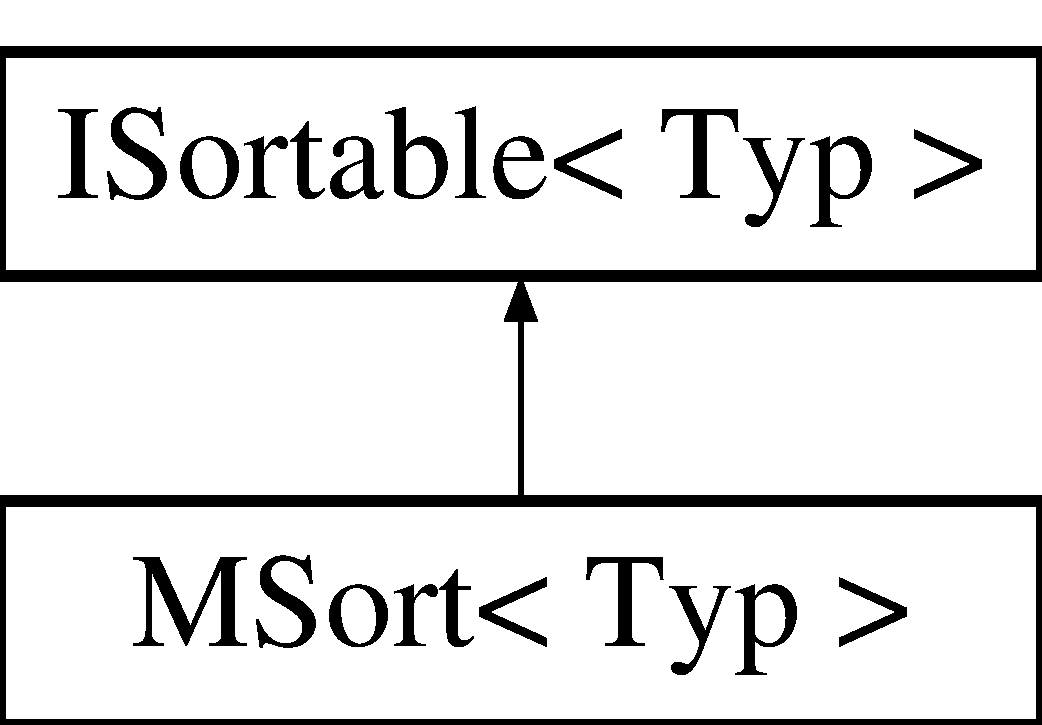
\includegraphics[height=2.000000cm]{class_m_sort}
\end{center}
\end{figure}
\subsection*{Public Member Functions}
\begin{DoxyCompactItemize}
\item 
void \hyperlink{class_m_sort_a90bfe37f7a17b529b97abba47495ab9a}{\-\_\-\-Sort} (\hyperlink{class_iterable}{Iterable}$<$ Typ $>$ $\ast$Kontener)
\begin{DoxyCompactList}\small\item\em Metoda inicjalizujaca sortowanie przez scalanie. \end{DoxyCompactList}\end{DoxyCompactItemize}
\subsection*{Private Member Functions}
\begin{DoxyCompactItemize}
\item 
void \hyperlink{class_m_sort_a2bc5e52492763e452c81d252a2e16a46}{Msort} (Typ $\ast$T, int p, int k, \hyperlink{class_iterable}{Iterable}$<$ Typ $>$ $\ast$K)
\begin{DoxyCompactList}\small\item\em Metoda Dzielaca tablice. \end{DoxyCompactList}\item 
void \hyperlink{class_m_sort_a04a2f5f2f3afc5337fe07e9f387dc291}{Merge} (Typ $\ast$Temp, int l, int s, int p, \hyperlink{class_iterable}{Iterable}$<$ Typ $>$ $\ast$K)
\begin{DoxyCompactList}\small\item\em Metoda Dzielaca tablice. \end{DoxyCompactList}\end{DoxyCompactItemize}


\subsection{Detailed Description}
\subsubsection*{template$<$class Typ$>$class M\-Sort$<$ Typ $>$}

Modeluje sortowanie przez scalanie. 

Klasa zawiera implementacje algorytmu sortowania przez scalanie 

\subsection{Member Function Documentation}
\hypertarget{class_m_sort_a90bfe37f7a17b529b97abba47495ab9a}{\index{M\-Sort@{M\-Sort}!\-\_\-\-Sort@{\-\_\-\-Sort}}
\index{\-\_\-\-Sort@{\-\_\-\-Sort}!MSort@{M\-Sort}}
\subsubsection[{\-\_\-\-Sort}]{\setlength{\rightskip}{0pt plus 5cm}template$<$class Typ $>$ void {\bf M\-Sort}$<$ Typ $>$\-::\-\_\-\-Sort (
\begin{DoxyParamCaption}
\item[{{\bf Iterable}$<$ Typ $>$ $\ast$}]{Kontener}
\end{DoxyParamCaption}
)\hspace{0.3cm}{\ttfamily [inline]}, {\ttfamily [virtual]}}}\label{class_m_sort_a90bfe37f7a17b529b97abba47495ab9a}


Metoda inicjalizujaca sortowanie przez scalanie. 

Metoda ma za zadanie zainicjalizowac algorytm sortowania przez scalanie dla wybranej struktury danych


\begin{DoxyParams}[1]{Parameters}
\mbox{\tt in}  & {\em Kontener} & -\/ rodzaj kontenera,ktory zostanie posortowany \\
\hline
\end{DoxyParams}


Implements \hyperlink{class_i_sortable_aca218e19355fb5d0e6ac7b29ea17dc59}{I\-Sortable$<$ Typ $>$}.

\hypertarget{class_m_sort_a04a2f5f2f3afc5337fe07e9f387dc291}{\index{M\-Sort@{M\-Sort}!Merge@{Merge}}
\index{Merge@{Merge}!MSort@{M\-Sort}}
\subsubsection[{Merge}]{\setlength{\rightskip}{0pt plus 5cm}template$<$class Typ $>$ void {\bf M\-Sort}$<$ Typ $>$\-::Merge (
\begin{DoxyParamCaption}
\item[{Typ $\ast$}]{Temp, }
\item[{int}]{l, }
\item[{int}]{s, }
\item[{int}]{p, }
\item[{{\bf Iterable}$<$ Typ $>$ $\ast$}]{K}
\end{DoxyParamCaption}
)\hspace{0.3cm}{\ttfamily [inline]}, {\ttfamily [private]}}}\label{class_m_sort_a04a2f5f2f3afc5337fe07e9f387dc291}


Metoda Dzielaca tablice. 

Metoda ma za zadanie przekopiowac zawartosc zbiotu glownego do tablicy tymczasowej.\-Nastepnie operujac na kopii ustawia wskazniki na poczatki kolejnych zbiorow i porownywane sa wskaane wartosci. Mniejsze wpisujemy do zbioru glownego i przesuwamy odpowiedni wskaznik Czynnos wykonujemy rekurencyjnie az do momentu gdy jeden ze wskaznikow osiagnie koniec zbioru


\begin{DoxyParams}[1]{Parameters}
\mbox{\tt in}  & {\em Temp} & -\/ Wskaznik na tablice pomocnicza \\
\hline
\mbox{\tt in}  & {\em l} & -\/ Poczatkowy indeks tablicy \\
\hline
\mbox{\tt in}  & {\em s} & -\/ Srodkowy indeks tablicy \\
\hline
\mbox{\tt in}  & {\em p} & -\/ Koncowy indks tablicy \\
\hline
\end{DoxyParams}
\hypertarget{class_m_sort_a2bc5e52492763e452c81d252a2e16a46}{\index{M\-Sort@{M\-Sort}!Msort@{Msort}}
\index{Msort@{Msort}!MSort@{M\-Sort}}
\subsubsection[{Msort}]{\setlength{\rightskip}{0pt plus 5cm}template$<$class Typ $>$ void {\bf M\-Sort}$<$ Typ $>$\-::Msort (
\begin{DoxyParamCaption}
\item[{Typ $\ast$}]{T, }
\item[{int}]{p, }
\item[{int}]{k, }
\item[{{\bf Iterable}$<$ Typ $>$ $\ast$}]{K}
\end{DoxyParamCaption}
)\hspace{0.3cm}{\ttfamily [inline]}, {\ttfamily [private]}}}\label{class_m_sort_a2bc5e52492763e452c81d252a2e16a46}


Metoda Dzielaca tablice. 

Metoda ma za zadanie przekopiowac zawartosc zbiotu glownego do tablicy tymczasowej.\-Nastepnie operujac na kopii ustawia wskazniki na poczatki kolejnych zbiorow i porownywane sa wskaane wartosci. Mniejsze wpisujemy do zbioru glownego i przesuwamy odpowiedni wskaznik Czynnos wykonujemy rekurencyjnie az do momentu gdy jeden ze wskaznikow osiagnie koniec zbioru


\begin{DoxyParams}[1]{Parameters}
\mbox{\tt in}  & {\em Temp} & -\/ Wskaznik na tablice pomocnicza \\
\hline
\mbox{\tt in}  & {\em l} & -\/ Poczatkowy indeks tablicy \\
\hline
\mbox{\tt in}  & {\em s} & -\/ Srodkowy indeks tablicy \\
\hline
\mbox{\tt in}  & {\em p} & -\/ Koncowy indks tablicy \\
\hline
\end{DoxyParams}


The documentation for this class was generated from the following file\-:\begin{DoxyCompactItemize}
\item 
/home/bartolomeo/209296/prj/inc/\hyperlink{_m_sort_8hh}{M\-Sort.\-hh}\end{DoxyCompactItemize}

\hypertarget{class_q_sort}{\section{Q\-Sort$<$ Typ $>$ Class Template Reference}
\label{class_q_sort}\index{Q\-Sort$<$ Typ $>$@{Q\-Sort$<$ Typ $>$}}
}


Modeluje sortowanie szybkie.  




{\ttfamily \#include $<$Q\-Sort.\-hh$>$}

Inheritance diagram for Q\-Sort$<$ Typ $>$\-:\begin{figure}[H]
\begin{center}
\leavevmode
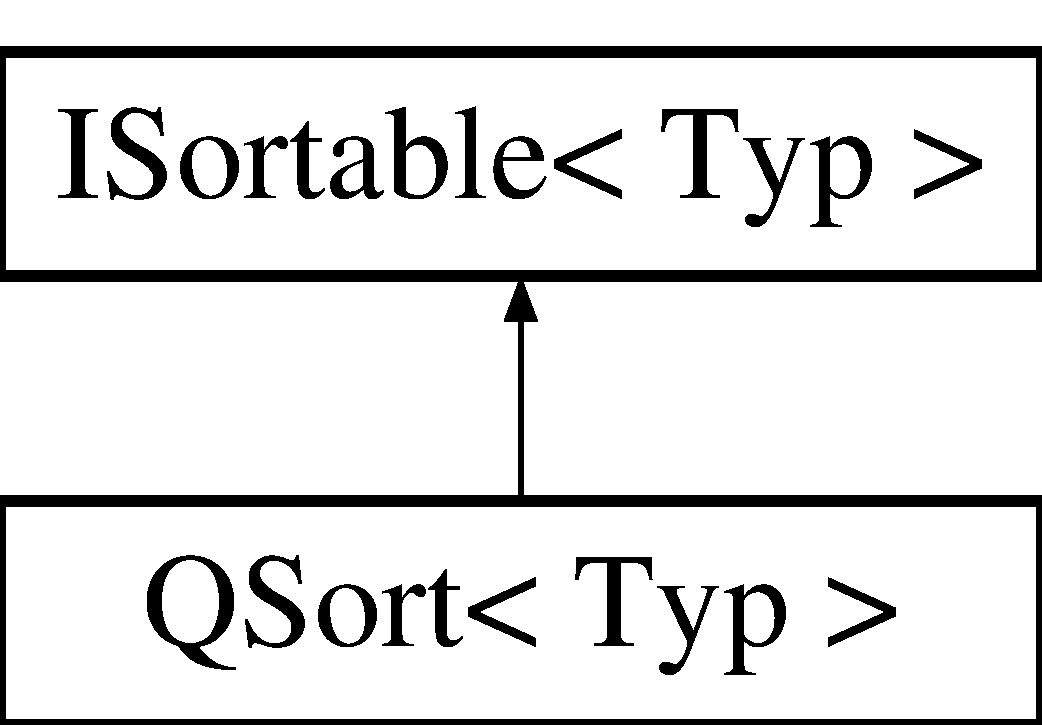
\includegraphics[height=2.000000cm]{class_q_sort}
\end{center}
\end{figure}
\subsection*{Public Member Functions}
\begin{DoxyCompactItemize}
\item 
void \hyperlink{class_q_sort_a059dc69db4a44032648c766e20c92126}{\-\_\-\-Sort} (\hyperlink{class_iterable}{Iterable}$<$ Typ $>$ $\ast$Kontener)
\begin{DoxyCompactList}\small\item\em Metoda inicjalizujaca sortowanie szybkie. \end{DoxyCompactList}\end{DoxyCompactItemize}
\subsection*{Private Member Functions}
\begin{DoxyCompactItemize}
\item 
void \hyperlink{class_q_sort_ad65785cc38373aa2ac7750c26b85cdd3}{Qsort} (int l, int h, \hyperlink{class_iterable}{Iterable}$<$ Typ $>$ $\ast$K)
\begin{DoxyCompactList}\small\item\em Metoda bedaca implementacja algorytmu sortowania szybkiego. \end{DoxyCompactList}\item 
int \hyperlink{class_q_sort_ae579d127add3ee9b5a004752fee8d20c}{Partycjowanie} (int p, int k, \hyperlink{class_iterable}{Iterable}$<$ Typ $>$ $\ast$K)
\begin{DoxyCompactList}\small\item\em Metoda segregujaca. \end{DoxyCompactList}\end{DoxyCompactItemize}


\subsection{Detailed Description}
\subsubsection*{template$<$class Typ$>$class Q\-Sort$<$ Typ $>$}

Modeluje sortowanie szybkie. 

Klasa zawiera implementacje algorytmu sortowania szybkiego 

\subsection{Member Function Documentation}
\hypertarget{class_q_sort_a059dc69db4a44032648c766e20c92126}{\index{Q\-Sort@{Q\-Sort}!\-\_\-\-Sort@{\-\_\-\-Sort}}
\index{\-\_\-\-Sort@{\-\_\-\-Sort}!QSort@{Q\-Sort}}
\subsubsection[{\-\_\-\-Sort}]{\setlength{\rightskip}{0pt plus 5cm}template$<$class Typ $>$ void {\bf Q\-Sort}$<$ Typ $>$\-::\-\_\-\-Sort (
\begin{DoxyParamCaption}
\item[{{\bf Iterable}$<$ Typ $>$ $\ast$}]{Kontener}
\end{DoxyParamCaption}
)\hspace{0.3cm}{\ttfamily [inline]}, {\ttfamily [virtual]}}}\label{class_q_sort_a059dc69db4a44032648c766e20c92126}


Metoda inicjalizujaca sortowanie szybkie. 

Metoda ma za zadanie zainicjalizowac algorytm sortowania szybkiego dla wybranej struktury danych


\begin{DoxyParams}[1]{Parameters}
\mbox{\tt in}  & {\em Kontener} & -\/ rodzaj kontenera,ktory zostanie posortowany \\
\hline
\end{DoxyParams}


Implements \hyperlink{class_i_sortable_aca218e19355fb5d0e6ac7b29ea17dc59}{I\-Sortable$<$ Typ $>$}.

\hypertarget{class_q_sort_ae579d127add3ee9b5a004752fee8d20c}{\index{Q\-Sort@{Q\-Sort}!Partycjowanie@{Partycjowanie}}
\index{Partycjowanie@{Partycjowanie}!QSort@{Q\-Sort}}
\subsubsection[{Partycjowanie}]{\setlength{\rightskip}{0pt plus 5cm}template$<$class Typ $>$ int {\bf Q\-Sort}$<$ Typ $>$\-::Partycjowanie (
\begin{DoxyParamCaption}
\item[{int}]{p, }
\item[{int}]{k, }
\item[{{\bf Iterable}$<$ Typ $>$ $\ast$}]{K}
\end{DoxyParamCaption}
)\hspace{0.3cm}{\ttfamily [inline]}, {\ttfamily [private]}}}\label{class_q_sort_ae579d127add3ee9b5a004752fee8d20c}


Metoda segregujaca. 

Metoda ma za zadanie wybor elementu, ktory ma byc uzyty do podzialu i przenosi wszytskie elementy mniejsze na lewo od tego elementu, a wieksze elementy na prawo od wybranego elementu 
\begin{DoxyParams}[1]{Parameters}
\mbox{\tt in}  & {\em p} & -\/ poczatkowy indeks podzbiotru \\
\hline
\mbox{\tt in}  & {\em k} & -\/ koncowy indeks podzbioru \\
\hline
\end{DoxyParams}
\begin{DoxyReturn}{Returns}

\end{DoxyReturn}
\hypertarget{class_q_sort_ad65785cc38373aa2ac7750c26b85cdd3}{\index{Q\-Sort@{Q\-Sort}!Qsort@{Qsort}}
\index{Qsort@{Qsort}!QSort@{Q\-Sort}}
\subsubsection[{Qsort}]{\setlength{\rightskip}{0pt plus 5cm}template$<$class Typ $>$ void {\bf Q\-Sort}$<$ Typ $>$\-::Qsort (
\begin{DoxyParamCaption}
\item[{int}]{l, }
\item[{int}]{h, }
\item[{{\bf Iterable}$<$ Typ $>$ $\ast$}]{K}
\end{DoxyParamCaption}
)\hspace{0.3cm}{\ttfamily [inline]}, {\ttfamily [private]}}}\label{class_q_sort_ad65785cc38373aa2ac7750c26b85cdd3}


Metoda bedaca implementacja algorytmu sortowania szybkiego. 


\begin{DoxyParams}[1]{Parameters}
\mbox{\tt in}  & {\em l} & -\/ poczatkowy indeks tablicy \\
\hline
\mbox{\tt in}  & {\em h} & -\/ koncowy indeks tablicy \\
\hline
\end{DoxyParams}


The documentation for this class was generated from the following file\-:\begin{DoxyCompactItemize}
\item 
/home/bartolomeo/209296/prj/inc/\hyperlink{_q_sort_8hh}{Q\-Sort.\-hh}\end{DoxyCompactItemize}

\hypertarget{class_q_sort_opt}{\section{Q\-Sort\-Opt$<$ Typ $>$ Class Template Reference}
\label{class_q_sort_opt}\index{Q\-Sort\-Opt$<$ Typ $>$@{Q\-Sort\-Opt$<$ Typ $>$}}
}


Modeluje sortowanie szybkie z optymalizacja.  




{\ttfamily \#include $<$Q\-Sort\-Opt.\-hh$>$}

Inheritance diagram for Q\-Sort\-Opt$<$ Typ $>$\-:\begin{figure}[H]
\begin{center}
\leavevmode
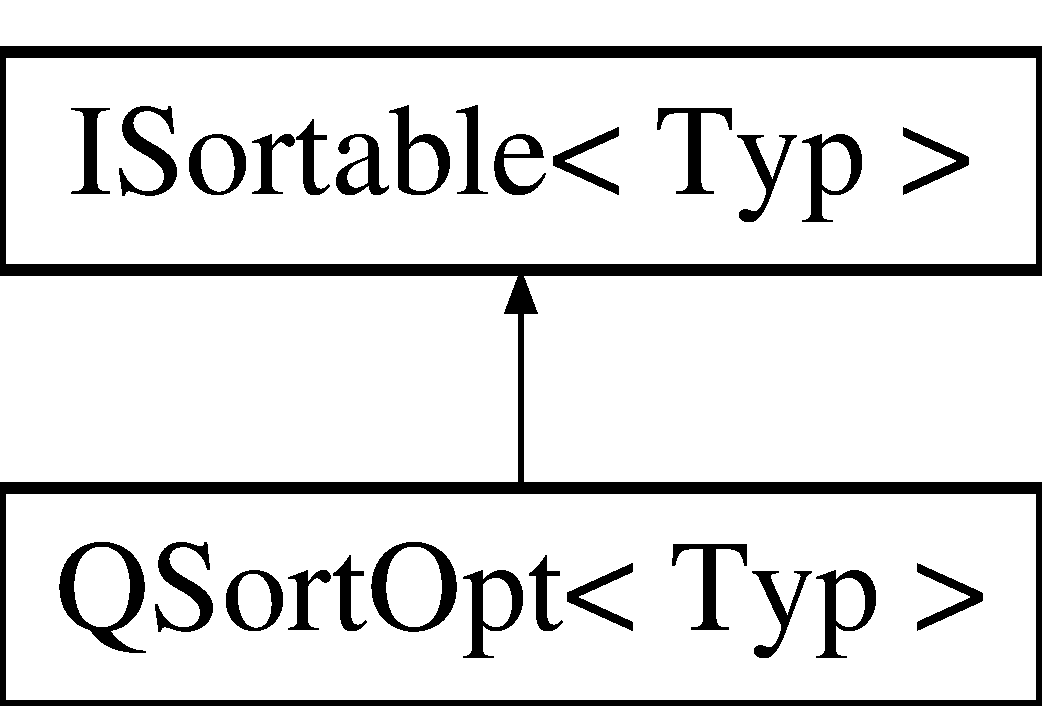
\includegraphics[height=2.000000cm]{class_q_sort_opt}
\end{center}
\end{figure}
\subsection*{Public Member Functions}
\begin{DoxyCompactItemize}
\item 
void \hyperlink{class_q_sort_opt_af9283edf949f7631c4f08f4b945370fa}{\-\_\-\-Sort} (\hyperlink{class_iterable}{Iterable}$<$ Typ $>$ $\ast$Kontener)
\begin{DoxyCompactList}\small\item\em Metoda inicjalizujaca sortowanie szybkie z optymalizacja. \end{DoxyCompactList}\end{DoxyCompactItemize}
\subsection*{Private Member Functions}
\begin{DoxyCompactItemize}
\item 
int \hyperlink{class_q_sort_opt_a1b932a3b24d6ae2c4228ac09abbdb751}{Partycjowanie} (int p, int k, \hyperlink{class_iterable}{Iterable}$<$ Typ $>$ $\ast$K)
\begin{DoxyCompactList}\small\item\em Zotymalizowane Sortowanie Szybkie. \end{DoxyCompactList}\item 
void \hyperlink{class_q_sort_opt_a546c6bd644e84d54f87d9788a6a34836}{Qsort\-Opt} (int lewy, int prawy1, \hyperlink{class_iterable}{Iterable}$<$ Typ $>$ $\ast$K)
\item 
int \hyperlink{class_q_sort_opt_a10a7caacd69153bad656cb022f00c806}{Mediana} (Typ $\ast$W) const 
\begin{DoxyCompactList}\small\item\em Mediana Metoda wyznaczajaca mediana dla tablicy 3 elementowej. Jest to metoda pomocnicza, wykorzystywana przy optymalizacji doboru pivotu w sortowaniu szybkim. \end{DoxyCompactList}\end{DoxyCompactItemize}


\subsection{Detailed Description}
\subsubsection*{template$<$class Typ$>$class Q\-Sort\-Opt$<$ Typ $>$}

Modeluje sortowanie szybkie z optymalizacja. 

Klasa zawiera implementacje algorytmu sortowania szybkiego z optymalizacja 

\subsection{Member Function Documentation}
\hypertarget{class_q_sort_opt_af9283edf949f7631c4f08f4b945370fa}{\index{Q\-Sort\-Opt@{Q\-Sort\-Opt}!\-\_\-\-Sort@{\-\_\-\-Sort}}
\index{\-\_\-\-Sort@{\-\_\-\-Sort}!QSortOpt@{Q\-Sort\-Opt}}
\subsubsection[{\-\_\-\-Sort}]{\setlength{\rightskip}{0pt plus 5cm}template$<$class Typ $>$ void {\bf Q\-Sort\-Opt}$<$ Typ $>$\-::\-\_\-\-Sort (
\begin{DoxyParamCaption}
\item[{{\bf Iterable}$<$ Typ $>$ $\ast$}]{Kontener}
\end{DoxyParamCaption}
)\hspace{0.3cm}{\ttfamily [inline]}, {\ttfamily [virtual]}}}\label{class_q_sort_opt_af9283edf949f7631c4f08f4b945370fa}


Metoda inicjalizujaca sortowanie szybkie z optymalizacja. 

Metoda ma za zadanie zainicjalizowac algorytm sortowania szybkiego z optymalizacja dla wybranej struktury danych


\begin{DoxyParams}[1]{Parameters}
\mbox{\tt in}  & {\em Kontener} & -\/ rodzaj kontenera,ktory zostanie posortowany \\
\hline
\end{DoxyParams}


Implements \hyperlink{class_i_sortable_aca218e19355fb5d0e6ac7b29ea17dc59}{I\-Sortable$<$ Typ $>$}.

\hypertarget{class_q_sort_opt_a10a7caacd69153bad656cb022f00c806}{\index{Q\-Sort\-Opt@{Q\-Sort\-Opt}!Mediana@{Mediana}}
\index{Mediana@{Mediana}!QSortOpt@{Q\-Sort\-Opt}}
\subsubsection[{Mediana}]{\setlength{\rightskip}{0pt plus 5cm}template$<$class Typ $>$ int {\bf Q\-Sort\-Opt}$<$ Typ $>$\-::Mediana (
\begin{DoxyParamCaption}
\item[{Typ $\ast$}]{W}
\end{DoxyParamCaption}
) const\hspace{0.3cm}{\ttfamily [inline]}, {\ttfamily [private]}}}\label{class_q_sort_opt_a10a7caacd69153bad656cb022f00c806}


Mediana Metoda wyznaczajaca mediana dla tablicy 3 elementowej. Jest to metoda pomocnicza, wykorzystywana przy optymalizacji doboru pivotu w sortowaniu szybkim. 

\begin{DoxyReturn}{Returns}
Zwraca indeks na ktorym znajduje sie mediana w tablicy wejsciowej 
\end{DoxyReturn}
\hypertarget{class_q_sort_opt_a1b932a3b24d6ae2c4228ac09abbdb751}{\index{Q\-Sort\-Opt@{Q\-Sort\-Opt}!Partycjowanie@{Partycjowanie}}
\index{Partycjowanie@{Partycjowanie}!QSortOpt@{Q\-Sort\-Opt}}
\subsubsection[{Partycjowanie}]{\setlength{\rightskip}{0pt plus 5cm}template$<$class Typ $>$ int {\bf Q\-Sort\-Opt}$<$ Typ $>$\-::Partycjowanie (
\begin{DoxyParamCaption}
\item[{int}]{p, }
\item[{int}]{k, }
\item[{{\bf Iterable}$<$ Typ $>$ $\ast$}]{K}
\end{DoxyParamCaption}
)\hspace{0.3cm}{\ttfamily [inline]}, {\ttfamily [private]}}}\label{class_q_sort_opt_a1b932a3b24d6ae2c4228ac09abbdb751}


Zotymalizowane Sortowanie Szybkie. 

Metoda modeluje algorytm sorotwanie szybkiego z zaimplementowanym algorytmem doboru pivotu, tak aby nie zostal wybrany najmniejszy element w danym podzbiorze.

\mbox{[}in\mbox{]} lewy -\/ poczatkowy indeks pozbioru 
\begin{DoxyParams}[1]{Parameters}
\mbox{\tt in}  & {\em prawy} & -\/ koncowy indeks podzbioru \\
\hline
\end{DoxyParams}
\hypertarget{class_q_sort_opt_a546c6bd644e84d54f87d9788a6a34836}{\index{Q\-Sort\-Opt@{Q\-Sort\-Opt}!Qsort\-Opt@{Qsort\-Opt}}
\index{Qsort\-Opt@{Qsort\-Opt}!QSortOpt@{Q\-Sort\-Opt}}
\subsubsection[{Qsort\-Opt}]{\setlength{\rightskip}{0pt plus 5cm}template$<$class Typ $>$ void {\bf Q\-Sort\-Opt}$<$ Typ $>$\-::Qsort\-Opt (
\begin{DoxyParamCaption}
\item[{int}]{lewy, }
\item[{int}]{prawy1, }
\item[{{\bf Iterable}$<$ Typ $>$ $\ast$}]{K}
\end{DoxyParamCaption}
)\hspace{0.3cm}{\ttfamily [inline]}, {\ttfamily [private]}}}\label{class_q_sort_opt_a546c6bd644e84d54f87d9788a6a34836}


The documentation for this class was generated from the following file\-:\begin{DoxyCompactItemize}
\item 
/home/bartolomeo/209296/prj/inc/\hyperlink{_q_sort_opt_8hh}{Q\-Sort\-Opt.\-hh}\end{DoxyCompactItemize}

\hypertarget{class_stos_tab}{\section{Stos\-Tab$<$ Typ $>$ Class Template Reference}
\label{class_stos_tab}\index{Stos\-Tab$<$ Typ $>$@{Stos\-Tab$<$ Typ $>$}}
}


{\ttfamily \#include $<$Stos\-Tab.\-hh$>$}

Inheritance diagram for Stos\-Tab$<$ Typ $>$\-:\begin{figure}[H]
\begin{center}
\leavevmode
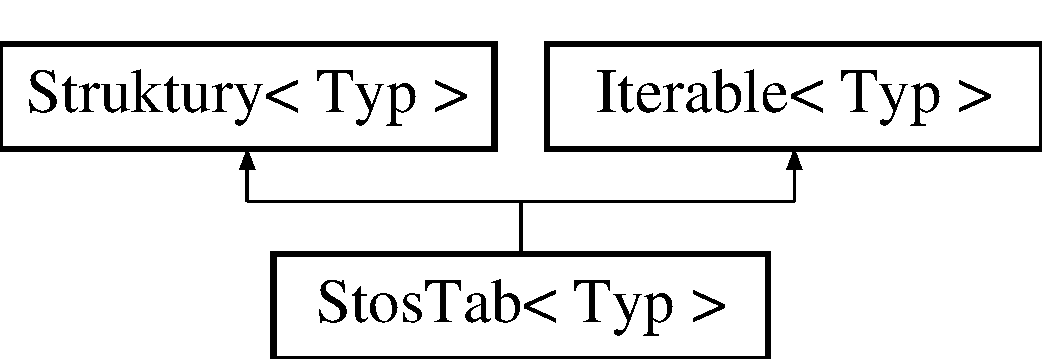
\includegraphics[height=2.000000cm]{class_stos_tab}
\end{center}
\end{figure}
\subsection*{Public Member Functions}
\begin{DoxyCompactItemize}
\item 
void \hyperlink{class_stos_tab_aec0cb259c6f044fa7d3b367dc1baca5c}{\-\_\-\-Zwolnij} ()
\item 
\hyperlink{class_stos_tab_a347bc350ea6ff8ad86b853895db5e7a9}{Stos\-Tab} ()
\begin{DoxyCompactList}\small\item\em Konstruktor Podczas tworzenia obiektu tej klasy automatycznie alokowana jest tablica o rozmiarze 1 oraz ustawienie obecnej liczby elementow listy na 0. \end{DoxyCompactList}\item 
\hyperlink{class_stos_tab_a5972345c1b71597d11330f8953dec03d}{Stos\-Tab} (const \hyperlink{class_stos_tab}{Stos\-Tab} \&K)
\begin{DoxyCompactList}\small\item\em Konstruktor Kopiujacy. \end{DoxyCompactList}\item 
virtual \hyperlink{class_stos_tab_a580b0a918a829377698f475a5f75457b}{$\sim$\-Stos\-Tab} ()
\begin{DoxyCompactList}\small\item\em Destruktor obiektu. \end{DoxyCompactList}\item 
void \hyperlink{class_stos_tab_a1b3c30902f28bf819ea5864c85ebede9}{\-\_\-\-Pokaz} () const 
\begin{DoxyCompactList}\small\item\em Metoda wypisujaca elemeny Stosu. \end{DoxyCompactList}\item 
Typ \hyperlink{class_stos_tab_a43e5e031570e69dc27fc11feca969645}{\-\_\-\-Pop} (unsigned int Pozycja=0)
\begin{DoxyCompactList}\small\item\em Metoda sciagajaca element ze stosu. \end{DoxyCompactList}\item 
void \hyperlink{class_stos_tab_a73c95fc8151510c21c5567e85296ea31}{\-\_\-\-Push} (Typ k, unsigned int Pozycja=0)
\begin{DoxyCompactList}\small\item\em Metoda dodajaca elemet do tablicy. \end{DoxyCompactList}\item 
unsigned int \hyperlink{class_stos_tab_a51b2da61d6c4c2085646b84395c2d3c0}{\-\_\-\-Rozmiar} () const 
\begin{DoxyCompactList}\small\item\em Metoda zwracajaca rozmiar listy. \end{DoxyCompactList}\item 
const Typ \hyperlink{class_stos_tab_aeae02936cdfdb3df20084174817b85dd}{Wartosc} (unsigned int Index) const 
\begin{DoxyCompactList}\small\item\em Metoda zwracajaca wartosc. \end{DoxyCompactList}\item 
Typ \& \hyperlink{class_stos_tab_ad19a954bb9cc9c32b42e4046c422984a}{Adres} (unsigned int Index)
\begin{DoxyCompactList}\small\item\em Metoda zwracajaca referencje. \end{DoxyCompactList}\item 
void \hyperlink{class_stos_tab_a6ce0e7f4dabae776f69fb0540ff7d8a4}{\-\_\-\-Zamien} (unsigned int i, unsigned int j)
\begin{DoxyCompactList}\small\item\em Metoda zamieniajaca Metoda ma za zadanie zamienic miejscami elementy wybrane przez argumenty wywolania. \end{DoxyCompactList}\end{DoxyCompactItemize}
\subsection*{Private Attributes}
\begin{DoxyCompactItemize}
\item 
Typ $\ast$ \hyperlink{class_stos_tab_ab6a9150fc50f2eb508a6c8026816631b}{\-\_\-\-L}
\begin{DoxyCompactList}\small\item\em Pole klasy \hyperlink{class_stos_tab}{Stos\-Tab}. \end{DoxyCompactList}\item 
unsigned int \hyperlink{class_stos_tab_abb7d52d46fdaf90dc2f3acb421bf7af6}{\-\_\-\-Rozmiar\-L}
\begin{DoxyCompactList}\small\item\em Pole Klasy \hyperlink{class_stos_tab}{Stos\-Tab}. \end{DoxyCompactList}\item 
unsigned int \hyperlink{class_stos_tab_a4db33c7f5b5f57b4d755a1beb59852dc}{\-\_\-\-Rozmiar\-T}
\begin{DoxyCompactList}\small\item\em Pole Klasy \hyperlink{class_stos_tab}{Stos\-Tab}. \end{DoxyCompactList}\end{DoxyCompactItemize}


\subsection{Constructor \& Destructor Documentation}
\hypertarget{class_stos_tab_a347bc350ea6ff8ad86b853895db5e7a9}{\index{Stos\-Tab@{Stos\-Tab}!Stos\-Tab@{Stos\-Tab}}
\index{Stos\-Tab@{Stos\-Tab}!StosTab@{Stos\-Tab}}
\subsubsection[{Stos\-Tab}]{\setlength{\rightskip}{0pt plus 5cm}template$<$class Typ $>$ {\bf Stos\-Tab}$<$ Typ $>$\-::{\bf Stos\-Tab} (
\begin{DoxyParamCaption}
{}
\end{DoxyParamCaption}
)\hspace{0.3cm}{\ttfamily [inline]}}}\label{class_stos_tab_a347bc350ea6ff8ad86b853895db5e7a9}


Konstruktor Podczas tworzenia obiektu tej klasy automatycznie alokowana jest tablica o rozmiarze 1 oraz ustawienie obecnej liczby elementow listy na 0. 

\hypertarget{class_stos_tab_a5972345c1b71597d11330f8953dec03d}{\index{Stos\-Tab@{Stos\-Tab}!Stos\-Tab@{Stos\-Tab}}
\index{Stos\-Tab@{Stos\-Tab}!StosTab@{Stos\-Tab}}
\subsubsection[{Stos\-Tab}]{\setlength{\rightskip}{0pt plus 5cm}template$<$class Typ $>$ {\bf Stos\-Tab}$<$ Typ $>$\-::{\bf Stos\-Tab} (
\begin{DoxyParamCaption}
\item[{const {\bf Stos\-Tab}$<$ Typ $>$ \&}]{K}
\end{DoxyParamCaption}
)\hspace{0.3cm}{\ttfamily [inline]}}}\label{class_stos_tab_a5972345c1b71597d11330f8953dec03d}


Konstruktor Kopiujacy. 

\hypertarget{class_stos_tab_a580b0a918a829377698f475a5f75457b}{\index{Stos\-Tab@{Stos\-Tab}!$\sim$\-Stos\-Tab@{$\sim$\-Stos\-Tab}}
\index{$\sim$\-Stos\-Tab@{$\sim$\-Stos\-Tab}!StosTab@{Stos\-Tab}}
\subsubsection[{$\sim$\-Stos\-Tab}]{\setlength{\rightskip}{0pt plus 5cm}template$<$class Typ $>$ virtual {\bf Stos\-Tab}$<$ Typ $>$\-::$\sim${\bf Stos\-Tab} (
\begin{DoxyParamCaption}
{}
\end{DoxyParamCaption}
)\hspace{0.3cm}{\ttfamily [inline]}}}\label{class_stos_tab_a580b0a918a829377698f475a5f75457b}


Destruktor obiektu. 



\subsection{Member Function Documentation}
\hypertarget{class_stos_tab_a1b3c30902f28bf819ea5864c85ebede9}{\index{Stos\-Tab@{Stos\-Tab}!\-\_\-\-Pokaz@{\-\_\-\-Pokaz}}
\index{\-\_\-\-Pokaz@{\-\_\-\-Pokaz}!StosTab@{Stos\-Tab}}
\subsubsection[{\-\_\-\-Pokaz}]{\setlength{\rightskip}{0pt plus 5cm}template$<$class Typ $>$ void {\bf Stos\-Tab}$<$ Typ $>$\-::\-\_\-\-Pokaz (
\begin{DoxyParamCaption}
{}
\end{DoxyParamCaption}
) const\hspace{0.3cm}{\ttfamily [inline]}, {\ttfamily [virtual]}}}\label{class_stos_tab_a1b3c30902f28bf819ea5864c85ebede9}


Metoda wypisujaca elemeny Stosu. 

Metoda ma za zadanie wypisac wszystkie elementy znajdujace sie obecnie na liscie danych 

Implements \hyperlink{class_struktury_a9a4290d332a6a613f92d4d4bfe2577ae}{Struktury$<$ Typ $>$}.

\hypertarget{class_stos_tab_a43e5e031570e69dc27fc11feca969645}{\index{Stos\-Tab@{Stos\-Tab}!\-\_\-\-Pop@{\-\_\-\-Pop}}
\index{\-\_\-\-Pop@{\-\_\-\-Pop}!StosTab@{Stos\-Tab}}
\subsubsection[{\-\_\-\-Pop}]{\setlength{\rightskip}{0pt plus 5cm}template$<$class Typ $>$ Typ {\bf Stos\-Tab}$<$ Typ $>$\-::\-\_\-\-Pop (
\begin{DoxyParamCaption}
\item[{unsigned int}]{Pozycja = {\ttfamily 0}}
\end{DoxyParamCaption}
)\hspace{0.3cm}{\ttfamily [inline]}, {\ttfamily [virtual]}}}\label{class_stos_tab_a43e5e031570e69dc27fc11feca969645}


Metoda sciagajaca element ze stosu. 

Metoda ma za zadanie sciagnac ostatni element stosu, w przypadku gdy tablica jest do połowy pusta nastepuje utworzenie nowej tablicy o dwa razy mniejszym rozmiarze 
\begin{DoxyParams}[1]{Parameters}
\mbox{\tt in}  & {\em Pozycja} & -\/ numer elementy kotry zostanie usuniety z listy i zostanie zwrocona jego wartosc\\
\hline
\end{DoxyParams}
\begin{DoxyReturn}{Returns}
Zwraca wybrany przez uzytkownika element 
\end{DoxyReturn}


Implements \hyperlink{class_struktury_a536345360bdb841d5462b578fe758b73}{Struktury$<$ Typ $>$}.

\hypertarget{class_stos_tab_a73c95fc8151510c21c5567e85296ea31}{\index{Stos\-Tab@{Stos\-Tab}!\-\_\-\-Push@{\-\_\-\-Push}}
\index{\-\_\-\-Push@{\-\_\-\-Push}!StosTab@{Stos\-Tab}}
\subsubsection[{\-\_\-\-Push}]{\setlength{\rightskip}{0pt plus 5cm}template$<$class Typ $>$ void {\bf Stos\-Tab}$<$ Typ $>$\-::\-\_\-\-Push (
\begin{DoxyParamCaption}
\item[{Typ}]{k, }
\item[{unsigned int}]{Pozycja = {\ttfamily 0}}
\end{DoxyParamCaption}
)\hspace{0.3cm}{\ttfamily [inline]}, {\ttfamily [virtual]}}}\label{class_stos_tab_a73c95fc8151510c21c5567e85296ea31}


Metoda dodajaca elemet do tablicy. 

Metoda ma za zadanie dodac nowy element na koncu stosu, w przypadku zapelnienia tablicy nastepuje utworzenie nowej tablicy i przepisanie elementow


\begin{DoxyParams}[1]{Parameters}
\mbox{\tt in}  & {\em k} & -\/ wartosc jaka chcemy dodac do listy \\
\hline
\mbox{\tt in}  & {\em Pozycja} & -\/ Pozycja na ktorej chcemy dodac wartosc \\
\hline
\end{DoxyParams}


Implements \hyperlink{class_struktury_aac09c019a75dd7bfda2f313733300c4c}{Struktury$<$ Typ $>$}.

\hypertarget{class_stos_tab_a51b2da61d6c4c2085646b84395c2d3c0}{\index{Stos\-Tab@{Stos\-Tab}!\-\_\-\-Rozmiar@{\-\_\-\-Rozmiar}}
\index{\-\_\-\-Rozmiar@{\-\_\-\-Rozmiar}!StosTab@{Stos\-Tab}}
\subsubsection[{\-\_\-\-Rozmiar}]{\setlength{\rightskip}{0pt plus 5cm}template$<$class Typ $>$ unsigned int {\bf Stos\-Tab}$<$ Typ $>$\-::\-\_\-\-Rozmiar (
\begin{DoxyParamCaption}
{}
\end{DoxyParamCaption}
) const\hspace{0.3cm}{\ttfamily [inline]}, {\ttfamily [virtual]}}}\label{class_stos_tab_a51b2da61d6c4c2085646b84395c2d3c0}


Metoda zwracajaca rozmiar listy. 

Metoda zwraca informacje o obecnej ilosci danych w strukturze

\begin{DoxyReturn}{Returns}
Zwraca ilosc elementow listy 
\end{DoxyReturn}


Implements \hyperlink{class_struktury_a3ed3c70e26cefc242633abc13097acce}{Struktury$<$ Typ $>$}.

\hypertarget{class_stos_tab_a6ce0e7f4dabae776f69fb0540ff7d8a4}{\index{Stos\-Tab@{Stos\-Tab}!\-\_\-\-Zamien@{\-\_\-\-Zamien}}
\index{\-\_\-\-Zamien@{\-\_\-\-Zamien}!StosTab@{Stos\-Tab}}
\subsubsection[{\-\_\-\-Zamien}]{\setlength{\rightskip}{0pt plus 5cm}template$<$class Typ $>$ void {\bf Stos\-Tab}$<$ Typ $>$\-::\-\_\-\-Zamien (
\begin{DoxyParamCaption}
\item[{unsigned int}]{i, }
\item[{unsigned int}]{j}
\end{DoxyParamCaption}
)\hspace{0.3cm}{\ttfamily [inline]}, {\ttfamily [virtual]}}}\label{class_stos_tab_a6ce0e7f4dabae776f69fb0540ff7d8a4}


Metoda zamieniajaca Metoda ma za zadanie zamienic miejscami elementy wybrane przez argumenty wywolania. 


\begin{DoxyParams}[1]{Parameters}
\mbox{\tt in}  & {\em i} & -\/ Adres elementu podlegajacy zamianie \\
\hline
\mbox{\tt in}  & {\em j} & -\/ Adres elementu podlegajacy zamianie \\
\hline
\end{DoxyParams}


Implements \hyperlink{class_iterable_a631b741c6f81ae09f823c86f9eed9f7b}{Iterable$<$ Typ $>$}.

\hypertarget{class_stos_tab_aec0cb259c6f044fa7d3b367dc1baca5c}{\index{Stos\-Tab@{Stos\-Tab}!\-\_\-\-Zwolnij@{\-\_\-\-Zwolnij}}
\index{\-\_\-\-Zwolnij@{\-\_\-\-Zwolnij}!StosTab@{Stos\-Tab}}
\subsubsection[{\-\_\-\-Zwolnij}]{\setlength{\rightskip}{0pt plus 5cm}template$<$class Typ $>$ void {\bf Stos\-Tab}$<$ Typ $>$\-::\-\_\-\-Zwolnij (
\begin{DoxyParamCaption}
{}
\end{DoxyParamCaption}
)\hspace{0.3cm}{\ttfamily [inline]}, {\ttfamily [virtual]}}}\label{class_stos_tab_aec0cb259c6f044fa7d3b367dc1baca5c}
Metoda zwalniajaca pamiec

Metoda ma za zadanie zwolnij pamiec zajmowana przez dane, dopoki ilosc elementow listy nie wynosi 0 wykonywana jest metoda \-\_\-\-Pop, aby oproznic stos i zwolnic pamiec 

Implements \hyperlink{class_struktury_aa85ab98de0f8bb1c257e6d1723d107f5}{Struktury$<$ Typ $>$}.

\hypertarget{class_stos_tab_ad19a954bb9cc9c32b42e4046c422984a}{\index{Stos\-Tab@{Stos\-Tab}!Adres@{Adres}}
\index{Adres@{Adres}!StosTab@{Stos\-Tab}}
\subsubsection[{Adres}]{\setlength{\rightskip}{0pt plus 5cm}template$<$class Typ $>$ Typ\& {\bf Stos\-Tab}$<$ Typ $>$\-::Adres (
\begin{DoxyParamCaption}
\item[{unsigned int}]{i}
\end{DoxyParamCaption}
)\hspace{0.3cm}{\ttfamily [inline]}, {\ttfamily [virtual]}}}\label{class_stos_tab_ad19a954bb9cc9c32b42e4046c422984a}


Metoda zwracajaca referencje. 

Metoda ma za zadanie zwrocic referencje do pola kontenera zadanego poprzez argument metody 

Implements \hyperlink{class_iterable_a7e56512db9ef2691198e1914a4ddb300}{Iterable$<$ Typ $>$}.

\hypertarget{class_stos_tab_aeae02936cdfdb3df20084174817b85dd}{\index{Stos\-Tab@{Stos\-Tab}!Wartosc@{Wartosc}}
\index{Wartosc@{Wartosc}!StosTab@{Stos\-Tab}}
\subsubsection[{Wartosc}]{\setlength{\rightskip}{0pt plus 5cm}template$<$class Typ $>$ const Typ {\bf Stos\-Tab}$<$ Typ $>$\-::Wartosc (
\begin{DoxyParamCaption}
\item[{unsigned int}]{i}
\end{DoxyParamCaption}
) const\hspace{0.3cm}{\ttfamily [inline]}, {\ttfamily [virtual]}}}\label{class_stos_tab_aeae02936cdfdb3df20084174817b85dd}


Metoda zwracajaca wartosc. 

Metoda ma za zadanei zwrocic wartosc,kryjaca sie pod danym indeksem dla dowolnego kontenera posiadajacego interfejs.


\begin{DoxyParams}[1]{Parameters}
\mbox{\tt in}  & {\em i} & -\/\-Indeks z ktorego zostanie odczytana wartosc\\
\hline
\end{DoxyParams}
\begin{DoxyReturn}{Returns}
Zwraca wartosc, kryjaca sie pod danym indeksem konteneru 
\end{DoxyReturn}


Implements \hyperlink{class_iterable_a6b75a7c8c41e1f13e6eff2276af62aeb}{Iterable$<$ Typ $>$}.



\subsection{Member Data Documentation}
\hypertarget{class_stos_tab_ab6a9150fc50f2eb508a6c8026816631b}{\index{Stos\-Tab@{Stos\-Tab}!\-\_\-\-L@{\-\_\-\-L}}
\index{\-\_\-\-L@{\-\_\-\-L}!StosTab@{Stos\-Tab}}
\subsubsection[{\-\_\-\-L}]{\setlength{\rightskip}{0pt plus 5cm}template$<$class Typ $>$ Typ$\ast$ {\bf Stos\-Tab}$<$ Typ $>$\-::\-\_\-\-L\hspace{0.3cm}{\ttfamily [private]}}}\label{class_stos_tab_ab6a9150fc50f2eb508a6c8026816631b}


Pole klasy \hyperlink{class_stos_tab}{Stos\-Tab}. 

Pole zawiera wskaznik na typ calkowity, sluzy do alokacji pamieci na dynamiczna tablice \hypertarget{class_stos_tab_abb7d52d46fdaf90dc2f3acb421bf7af6}{\index{Stos\-Tab@{Stos\-Tab}!\-\_\-\-Rozmiar\-L@{\-\_\-\-Rozmiar\-L}}
\index{\-\_\-\-Rozmiar\-L@{\-\_\-\-Rozmiar\-L}!StosTab@{Stos\-Tab}}
\subsubsection[{\-\_\-\-Rozmiar\-L}]{\setlength{\rightskip}{0pt plus 5cm}template$<$class Typ $>$ unsigned int {\bf Stos\-Tab}$<$ Typ $>$\-::\-\_\-\-Rozmiar\-L\hspace{0.3cm}{\ttfamily [private]}}}\label{class_stos_tab_abb7d52d46fdaf90dc2f3acb421bf7af6}


Pole Klasy \hyperlink{class_stos_tab}{Stos\-Tab}. 

Pole przechowuje informacje o ilosci obecnie znajdujacych sie elementow na liscie danych \hypertarget{class_stos_tab_a4db33c7f5b5f57b4d755a1beb59852dc}{\index{Stos\-Tab@{Stos\-Tab}!\-\_\-\-Rozmiar\-T@{\-\_\-\-Rozmiar\-T}}
\index{\-\_\-\-Rozmiar\-T@{\-\_\-\-Rozmiar\-T}!StosTab@{Stos\-Tab}}
\subsubsection[{\-\_\-\-Rozmiar\-T}]{\setlength{\rightskip}{0pt plus 5cm}template$<$class Typ $>$ unsigned int {\bf Stos\-Tab}$<$ Typ $>$\-::\-\_\-\-Rozmiar\-T\hspace{0.3cm}{\ttfamily [private]}}}\label{class_stos_tab_a4db33c7f5b5f57b4d755a1beb59852dc}


Pole Klasy \hyperlink{class_stos_tab}{Stos\-Tab}. 

Pole przechowuje informacje o obecnycm rozmiarze tablicy danych 

The documentation for this class was generated from the following file\-:\begin{DoxyCompactItemize}
\item 
/home/bartolomeo/209296/prj/inc/\hyperlink{_stos_tab_8hh}{Stos\-Tab.\-hh}\end{DoxyCompactItemize}

\hypertarget{class_struktury}{\section{Struktury$<$ Typ $>$ Class Template Reference}
\label{class_struktury}\index{Struktury$<$ Typ $>$@{Struktury$<$ Typ $>$}}
}


Modeluje pojecie \hyperlink{class_struktury}{Struktury} danych, klasa bazowa dla Stosu,Kolejki i Listy,zarowno w implemenetacji wskaznikowej jak i tablicowej.  




{\ttfamily \#include $<$I\-Struktury.\-hh$>$}

Inheritance diagram for Struktury$<$ Typ $>$\-:\begin{figure}[H]
\begin{center}
\leavevmode
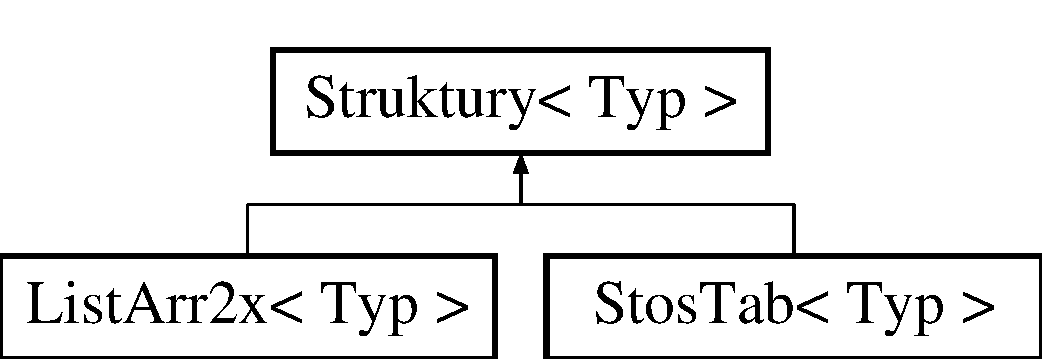
\includegraphics[height=2.000000cm]{class_struktury}
\end{center}
\end{figure}
\subsection*{Public Member Functions}
\begin{DoxyCompactItemize}
\item 
virtual void \hyperlink{class_struktury_aac09c019a75dd7bfda2f313733300c4c}{\-\_\-\-Push} (Typ k, unsigned int Pozycja)=0
\begin{DoxyCompactList}\small\item\em Metoda dodajaca kolejny element struktury. \end{DoxyCompactList}\item 
virtual Typ \hyperlink{class_struktury_a536345360bdb841d5462b578fe758b73}{\-\_\-\-Pop} (unsigned int Pozycja)=0
\begin{DoxyCompactList}\small\item\em Metoda usuwajaca element. \end{DoxyCompactList}\item 
virtual unsigned int \hyperlink{class_struktury_a3ed3c70e26cefc242633abc13097acce}{\-\_\-\-Rozmiar} () const =0
\begin{DoxyCompactList}\small\item\em Metoda zwracajaca rozmiar \hyperlink{class_struktury}{Struktury}. \end{DoxyCompactList}\item 
virtual void \hyperlink{class_struktury_a9a4290d332a6a613f92d4d4bfe2577ae}{\-\_\-\-Pokaz} () const =0
\begin{DoxyCompactList}\small\item\em Metoda wyswietlajaca dane. \end{DoxyCompactList}\item 
virtual void \hyperlink{class_struktury_aa85ab98de0f8bb1c257e6d1723d107f5}{\-\_\-\-Zwolnij} ()=0
\begin{DoxyCompactList}\small\item\em Metoda zwalniajaca pamiec. \end{DoxyCompactList}\end{DoxyCompactItemize}


\subsection{Detailed Description}
\subsubsection*{template$<$class Typ$>$class Struktury$<$ Typ $>$}

Modeluje pojecie \hyperlink{class_struktury}{Struktury} danych, klasa bazowa dla Stosu,Kolejki i Listy,zarowno w implemenetacji wskaznikowej jak i tablicowej. 

\subsection{Member Function Documentation}
\hypertarget{class_struktury_a9a4290d332a6a613f92d4d4bfe2577ae}{\index{Struktury@{Struktury}!\-\_\-\-Pokaz@{\-\_\-\-Pokaz}}
\index{\-\_\-\-Pokaz@{\-\_\-\-Pokaz}!Struktury@{Struktury}}
\subsubsection[{\-\_\-\-Pokaz}]{\setlength{\rightskip}{0pt plus 5cm}template$<$class Typ$>$ virtual void {\bf Struktury}$<$ Typ $>$\-::\-\_\-\-Pokaz (
\begin{DoxyParamCaption}
{}
\end{DoxyParamCaption}
) const\hspace{0.3cm}{\ttfamily [pure virtual]}}}\label{class_struktury_a9a4290d332a6a613f92d4d4bfe2577ae}


Metoda wyswietlajaca dane. 

Metoda ma za zadanie wyswietlic wszytskie dane nalezace do struktury 

Implemented in \hyperlink{class_list_arr2x_a1de6b30e511fef970573d06989bdbf30}{List\-Arr2x$<$ Typ $>$}, and \hyperlink{class_stos_tab_a1b3c30902f28bf819ea5864c85ebede9}{Stos\-Tab$<$ Typ $>$}.

\hypertarget{class_struktury_a536345360bdb841d5462b578fe758b73}{\index{Struktury@{Struktury}!\-\_\-\-Pop@{\-\_\-\-Pop}}
\index{\-\_\-\-Pop@{\-\_\-\-Pop}!Struktury@{Struktury}}
\subsubsection[{\-\_\-\-Pop}]{\setlength{\rightskip}{0pt plus 5cm}template$<$class Typ$>$ virtual Typ {\bf Struktury}$<$ Typ $>$\-::\-\_\-\-Pop (
\begin{DoxyParamCaption}
\item[{unsigned int}]{Pozycja}
\end{DoxyParamCaption}
)\hspace{0.3cm}{\ttfamily [pure virtual]}}}\label{class_struktury_a536345360bdb841d5462b578fe758b73}


Metoda usuwajaca element. 

Metoda ma za zadanie usunac element i w zaleznosci od implementowanej struktury bedzie to usuwany element usuwany z poczatk,końca lub w przypadku listy z dowolnego jej miejsca


\begin{DoxyParams}[1]{Parameters}
\mbox{\tt in}  & {\em Pozycja} & -\/ Numer elementu ,ktory zostanie dodany. Argument ma znaczenie tylko w przypadku listy i domyślnie jest ustawiony, tak aby element był dodawany zawsze na poczatku listy\\
\hline
\end{DoxyParams}
\begin{DoxyReturn}{Returns}
Zwraca wartosc elementu z odpowiedniego dla wybranej struktury miejsca 
\end{DoxyReturn}


Implemented in \hyperlink{class_list_arr2x_a4383548c83e707ba59d8d49ab051e8f8}{List\-Arr2x$<$ Typ $>$}, and \hyperlink{class_stos_tab_a43e5e031570e69dc27fc11feca969645}{Stos\-Tab$<$ Typ $>$}.

\hypertarget{class_struktury_aac09c019a75dd7bfda2f313733300c4c}{\index{Struktury@{Struktury}!\-\_\-\-Push@{\-\_\-\-Push}}
\index{\-\_\-\-Push@{\-\_\-\-Push}!Struktury@{Struktury}}
\subsubsection[{\-\_\-\-Push}]{\setlength{\rightskip}{0pt plus 5cm}template$<$class Typ$>$ virtual void {\bf Struktury}$<$ Typ $>$\-::\-\_\-\-Push (
\begin{DoxyParamCaption}
\item[{Typ}]{k, }
\item[{unsigned int}]{Pozycja}
\end{DoxyParamCaption}
)\hspace{0.3cm}{\ttfamily [pure virtual]}}}\label{class_struktury_aac09c019a75dd7bfda2f313733300c4c}


Metoda dodajaca kolejny element struktury. 

Metoda ma za zadanie dodac kolejny element do naszej struktury oraz zapisac w nim odpowiednia wartosc.\-W zaleznosci od implementowanej struktury element bedzie dodawany na poczatku lub na koncu struktury danych.


\begin{DoxyParams}[1]{Parameters}
\mbox{\tt in}  & {\em k} & -\/ wartosc typu calkowitnego, ktora bedzie umieszona w strukturze \\
\hline
\end{DoxyParams}


Implemented in \hyperlink{class_stos_tab_a73c95fc8151510c21c5567e85296ea31}{Stos\-Tab$<$ Typ $>$}, and \hyperlink{class_list_arr2x_aac4d1cdaa29d7d3d0a85aa469281d784}{List\-Arr2x$<$ Typ $>$}.

\hypertarget{class_struktury_a3ed3c70e26cefc242633abc13097acce}{\index{Struktury@{Struktury}!\-\_\-\-Rozmiar@{\-\_\-\-Rozmiar}}
\index{\-\_\-\-Rozmiar@{\-\_\-\-Rozmiar}!Struktury@{Struktury}}
\subsubsection[{\-\_\-\-Rozmiar}]{\setlength{\rightskip}{0pt plus 5cm}template$<$class Typ$>$ virtual unsigned int {\bf Struktury}$<$ Typ $>$\-::\-\_\-\-Rozmiar (
\begin{DoxyParamCaption}
{}
\end{DoxyParamCaption}
) const\hspace{0.3cm}{\ttfamily [pure virtual]}}}\label{class_struktury_a3ed3c70e26cefc242633abc13097acce}


Metoda zwracajaca rozmiar \hyperlink{class_struktury}{Struktury}. 

Metoda ma zadanie zwrocic bierzaca liczbe elementow nalezacych do danej struktury \begin{DoxyReturn}{Returns}
-\/ Bierzaca liczba elementow \hyperlink{class_struktury}{Struktury} danych 
\end{DoxyReturn}


Implemented in \hyperlink{class_list_arr2x_aa9d38356df7fec58f282ec00148bd6db}{List\-Arr2x$<$ Typ $>$}, and \hyperlink{class_stos_tab_a51b2da61d6c4c2085646b84395c2d3c0}{Stos\-Tab$<$ Typ $>$}.

\hypertarget{class_struktury_aa85ab98de0f8bb1c257e6d1723d107f5}{\index{Struktury@{Struktury}!\-\_\-\-Zwolnij@{\-\_\-\-Zwolnij}}
\index{\-\_\-\-Zwolnij@{\-\_\-\-Zwolnij}!Struktury@{Struktury}}
\subsubsection[{\-\_\-\-Zwolnij}]{\setlength{\rightskip}{0pt plus 5cm}template$<$class Typ$>$ virtual void {\bf Struktury}$<$ Typ $>$\-::\-\_\-\-Zwolnij (
\begin{DoxyParamCaption}
{}
\end{DoxyParamCaption}
)\hspace{0.3cm}{\ttfamily [pure virtual]}}}\label{class_struktury_aa85ab98de0f8bb1c257e6d1723d107f5}


Metoda zwalniajaca pamiec. 

Metoda ma za zadanie zwolnic pamiec uzywana przy zapelnienianiu danej struktry danymi 

Implemented in \hyperlink{class_list_arr2x_aec30c6d499f26d03e94e001e1358ee18}{List\-Arr2x$<$ Typ $>$}, and \hyperlink{class_stos_tab_aec0cb259c6f044fa7d3b367dc1baca5c}{Stos\-Tab$<$ Typ $>$}.



The documentation for this class was generated from the following file\-:\begin{DoxyCompactItemize}
\item 
/home/bartolomeo/209296/prj/inc/\hyperlink{_i_struktury_8hh}{I\-Struktury.\-hh}\end{DoxyCompactItemize}

\hypertarget{class_struktury_benchmark}{\section{Struktury\-Benchmark$<$ Typ $>$ Class Template Reference}
\label{class_struktury_benchmark}\index{Struktury\-Benchmark$<$ Typ $>$@{Struktury\-Benchmark$<$ Typ $>$}}
}


{\ttfamily \#include $<$Struktury\-Benchmark.\-hh$>$}

Inheritance diagram for Struktury\-Benchmark$<$ Typ $>$\-:\begin{figure}[H]
\begin{center}
\leavevmode
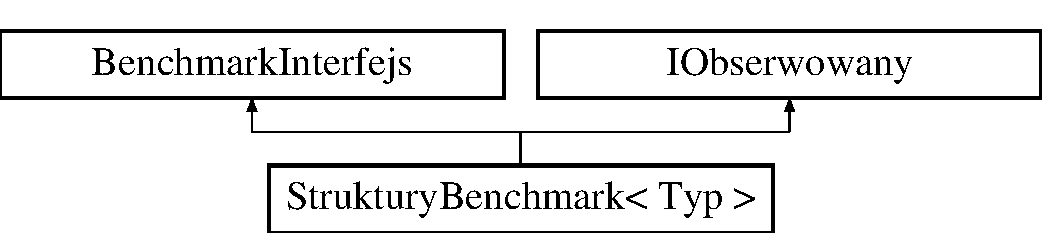
\includegraphics[height=2.000000cm]{class_struktury_benchmark}
\end{center}
\end{figure}
\subsection*{Public Member Functions}
\begin{DoxyCompactItemize}
\item 
\hyperlink{class_struktury_benchmark_a7fee46e82c9b608cf799855f1013b9f8}{Struktury\-Benchmark} (const unsigned int Proby, const unsigned int Powt, unsigned int $\ast$Rozmiary)
\begin{DoxyCompactList}\small\item\em Konstruktor obiektu. \end{DoxyCompactList}\item 
void \hyperlink{class_struktury_benchmark_a1eae568d916544c7ceb7a8ec071b17ff}{\-\_\-\-Wykonaj\-Test} ()
\begin{DoxyCompactList}\small\item\em Metoda inicjalizujaca test. \end{DoxyCompactList}\item 
void \hyperlink{class_struktury_benchmark_a92c72eeea5ac0da73a6f9f186a583294}{\-\_\-\-Ustaw} (\hyperlink{class_i_sortable}{I\-Sortable}$<$ Typ $>$ $\ast$A, \hyperlink{class_struktury}{Struktury}$<$ Typ $>$ $\ast$B, \hyperlink{class_iterable}{Iterable}$<$ Typ $>$ $\ast$C)
\begin{DoxyCompactList}\small\item\em Metoda Ustawiajaca. \end{DoxyCompactList}\item 
void \hyperlink{class_struktury_benchmark_a949e7eef56ff1dce1be1afac5fccc306}{\-\_\-\-Wczytaj} (string Plik\-Wart)
\begin{DoxyCompactList}\small\item\em Metoda Wczytujaca dane. \end{DoxyCompactList}\item 
void \hyperlink{class_struktury_benchmark_a63247cc5616565e429f5abd09d887630}{\-\_\-\-Dodaj\-Obserwator} (\hyperlink{class_i_obserwator}{I\-Obserwator} $\ast$O)
\begin{DoxyCompactList}\small\item\em Metoda dodajaca obserwator. \end{DoxyCompactList}\item 
void \hyperlink{class_struktury_benchmark_af08fe671ed7528428ffcb8a4daf65197}{\-\_\-\-Usun\-Obserwator} (\hyperlink{class_i_obserwator}{I\-Obserwator} $\ast$O)
\begin{DoxyCompactList}\small\item\em Metoda usuwajaca obserwator. \end{DoxyCompactList}\item 
void \hyperlink{class_struktury_benchmark_aa5a6c92b86be3cd99177322c92329164}{\-\_\-\-Generator} () const 
\begin{DoxyCompactList}\small\item\em Metoda generujaca dane. \end{DoxyCompactList}\end{DoxyCompactItemize}
\subsection*{Private Member Functions}
\begin{DoxyCompactItemize}
\item 
void \hyperlink{class_struktury_benchmark_a437a5c4b2a1811f3067d1117ac2c2c0e}{\-\_\-\-Test} () const 
\begin{DoxyCompactList}\small\item\em Metoda wykonujaca test dla odpowiedniej struktury. \end{DoxyCompactList}\item 
void \hyperlink{class_struktury_benchmark_a263ee44187c7efb212d031e97cd39bb1}{\-\_\-\-Zaladuj} (const unsigned int n) const 
\begin{DoxyCompactList}\small\item\em Metoda wypelniajaca Metoda ma za zadanie wypelnic dany kontener danymi. \end{DoxyCompactList}\item 
void \hyperlink{class_struktury_benchmark_a81596424109f9dbe028c3ad3496d04a1}{\-\_\-\-Zwolnij} ()
\begin{DoxyCompactList}\small\item\em Metoda zwalniajaca Pamiec. \end{DoxyCompactList}\item 
void \hyperlink{class_struktury_benchmark_af5aa09efcf9a1727e0868930b97ede49}{\-\_\-\-Powiadom\-Obserwatorow} ()
\begin{DoxyCompactList}\small\item\em Metoda informujaca obserwatorow. \end{DoxyCompactList}\end{DoxyCompactItemize}
\subsection*{Private Attributes}
\begin{DoxyCompactItemize}
\item 
\hyperlink{class_i_sortable}{I\-Sortable}$<$ Typ $>$ $\ast$ \hyperlink{class_struktury_benchmark_ab10e00df9ce397566d73f1a3697193f2}{I}
\begin{DoxyCompactList}\small\item\em Pole Strultury\-Benchmark Pole zawiera wskaźnik na interfejs sortujacy, za pomoca niego i metod wirtualnych beda wywolywane odpowiednie dla danej strktury metody. \end{DoxyCompactList}\item 
\hyperlink{class_struktury}{Struktury}$<$ Typ $>$ $\ast$ \hyperlink{class_struktury_benchmark_aa71bb2ddb1fb6f9e07ef8423c6225464}{S}
\begin{DoxyCompactList}\small\item\em Pole Strultury\-Benchmark Pole zawiera wskaźnik na \hyperlink{class_struktury}{Struktury}, za pomoca niego i metod wirtualnych beda wywolywane odpowiednie dla danej strktury metody. \end{DoxyCompactList}\item 
\hyperlink{class_iterable}{Iterable}$<$ Typ $>$ $\ast$ \hyperlink{class_struktury_benchmark_a1b7a323989d91e35099941977b688b22}{T}
\begin{DoxyCompactList}\small\item\em Pole Strultury\-Benchmark Pole zawiera wskaźnik na \hyperlink{class_iterable}{Iterable}, za pomoca niego i metod wirtualnych beda wywolywane odpowiednie dla danej strktury metody. \end{DoxyCompactList}\item 
int $\ast$ \hyperlink{class_struktury_benchmark_a98c2030555bbaa7fc7efe720bf22696c}{\-\_\-\-Wartosci}
\begin{DoxyCompactList}\small\item\em Pole Strktury\-Benchmark Pole zawiera wskaznik na typ calkowity, sluzy on do alokowania pamieci dla wczytanych z pliku danych. \end{DoxyCompactList}\item 
std\-::list$<$ \hyperlink{class_i_obserwator}{I\-Obserwator} $\ast$ $>$ \hyperlink{class_struktury_benchmark_a5c96eb86dfccdad59d41d478ca8d66c3}{Obserwatorzy}
\begin{DoxyCompactList}\small\item\em Pole \hyperlink{class_struktury_benchmark}{Struktury\-Benchmark}. \end{DoxyCompactList}\item 
unsigned int \hyperlink{class_struktury_benchmark_a5b2aee5eb235c0ad6c56a4871aad6bd3}{\-\_\-\-Ilosc\-Prob}
\begin{DoxyCompactList}\small\item\em Pole \hyperlink{class_struktury_benchmark}{Struktury\-Benchmark}. \end{DoxyCompactList}\item 
unsigned int \hyperlink{class_struktury_benchmark_a49d86123ea73ecc57bc161dcf40fba01}{\-\_\-\-Ilosc\-Powt}
\begin{DoxyCompactList}\small\item\em Pole \hyperlink{class_struktury_benchmark}{Struktury\-Benchmark}. \end{DoxyCompactList}\item 
unsigned int $\ast$ \hyperlink{class_struktury_benchmark_a9077a191d28f29d9b2eba8d4e8f72ce8}{\-\_\-\-Tablica\-Rozmiarow}
\begin{DoxyCompactList}\small\item\em Pole \hyperlink{class_struktury_benchmark}{Struktury\-Benchmark}. \end{DoxyCompactList}\item 
unsigned int \hyperlink{class_struktury_benchmark_a88384371e19a392f7d6d93a1ccadb115}{\-\_\-\-Ilosc\-Danych}
\begin{DoxyCompactList}\small\item\em Pole \hyperlink{class_struktury_benchmark}{Struktury\-Benchmark}. \end{DoxyCompactList}\end{DoxyCompactItemize}
\subsection*{Additional Inherited Members}


\subsection{Detailed Description}
\subsubsection*{template$<$class Typ$>$class Struktury\-Benchmark$<$ Typ $>$}

Klasa modeluje pojecie Benchmarku przeznaczonego dla struktur danych przechowujace dane 

\subsection{Constructor \& Destructor Documentation}
\hypertarget{class_struktury_benchmark_a7fee46e82c9b608cf799855f1013b9f8}{\index{Struktury\-Benchmark@{Struktury\-Benchmark}!Struktury\-Benchmark@{Struktury\-Benchmark}}
\index{Struktury\-Benchmark@{Struktury\-Benchmark}!StrukturyBenchmark@{Struktury\-Benchmark}}
\subsubsection[{Struktury\-Benchmark}]{\setlength{\rightskip}{0pt plus 5cm}template$<$class Typ $>$ {\bf Struktury\-Benchmark}$<$ Typ $>$\-::{\bf Struktury\-Benchmark} (
\begin{DoxyParamCaption}
\item[{const unsigned int}]{Proby, }
\item[{const unsigned int}]{Powt, }
\item[{unsigned int $\ast$}]{Rozmiary}
\end{DoxyParamCaption}
)\hspace{0.3cm}{\ttfamily [inline]}}}\label{class_struktury_benchmark_a7fee46e82c9b608cf799855f1013b9f8}


Konstruktor obiektu. 



\subsection{Member Function Documentation}
\hypertarget{class_struktury_benchmark_a63247cc5616565e429f5abd09d887630}{\index{Struktury\-Benchmark@{Struktury\-Benchmark}!\-\_\-\-Dodaj\-Obserwator@{\-\_\-\-Dodaj\-Obserwator}}
\index{\-\_\-\-Dodaj\-Obserwator@{\-\_\-\-Dodaj\-Obserwator}!StrukturyBenchmark@{Struktury\-Benchmark}}
\subsubsection[{\-\_\-\-Dodaj\-Obserwator}]{\setlength{\rightskip}{0pt plus 5cm}template$<$class Typ $>$ void {\bf Struktury\-Benchmark}$<$ Typ $>$\-::\-\_\-\-Dodaj\-Obserwator (
\begin{DoxyParamCaption}
\item[{{\bf I\-Obserwator} $\ast$}]{O}
\end{DoxyParamCaption}
)\hspace{0.3cm}{\ttfamily [inline]}, {\ttfamily [virtual]}}}\label{class_struktury_benchmark_a63247cc5616565e429f5abd09d887630}


Metoda dodajaca obserwator. 

Metoda ma za zadanie dodac nowego obserwatora do listy obserwatorow danego obiektu


\begin{DoxyParams}[1]{Parameters}
\mbox{\tt in}  & {\em O} & -\/ wskaznik na dodawany obserwator \\
\hline
\end{DoxyParams}


Implements \hyperlink{class_i_obserwowany_a3e7c49a1b168ed5a3f84bd0c5ae27513}{I\-Obserwowany}.

\hypertarget{class_struktury_benchmark_aa5a6c92b86be3cd99177322c92329164}{\index{Struktury\-Benchmark@{Struktury\-Benchmark}!\-\_\-\-Generator@{\-\_\-\-Generator}}
\index{\-\_\-\-Generator@{\-\_\-\-Generator}!StrukturyBenchmark@{Struktury\-Benchmark}}
\subsubsection[{\-\_\-\-Generator}]{\setlength{\rightskip}{0pt plus 5cm}template$<$class Typ $>$ void {\bf Struktury\-Benchmark}$<$ Typ $>$\-::\-\_\-\-Generator (
\begin{DoxyParamCaption}
{}
\end{DoxyParamCaption}
) const\hspace{0.3cm}{\ttfamily [inline]}, {\ttfamily [virtual]}}}\label{class_struktury_benchmark_aa5a6c92b86be3cd99177322c92329164}


Metoda generujaca dane. 

Metoda ma za zadanie wygenerowac pseudolosowe dane i zapisac je do pliku 

Implements \hyperlink{class_benchmark_interfejs_a69c431ffaa9d2ab995458cc8c6ae5c1f}{Benchmark\-Interfejs}.

\hypertarget{class_struktury_benchmark_af5aa09efcf9a1727e0868930b97ede49}{\index{Struktury\-Benchmark@{Struktury\-Benchmark}!\-\_\-\-Powiadom\-Obserwatorow@{\-\_\-\-Powiadom\-Obserwatorow}}
\index{\-\_\-\-Powiadom\-Obserwatorow@{\-\_\-\-Powiadom\-Obserwatorow}!StrukturyBenchmark@{Struktury\-Benchmark}}
\subsubsection[{\-\_\-\-Powiadom\-Obserwatorow}]{\setlength{\rightskip}{0pt plus 5cm}template$<$class Typ $>$ void {\bf Struktury\-Benchmark}$<$ Typ $>$\-::\-\_\-\-Powiadom\-Obserwatorow (
\begin{DoxyParamCaption}
{}
\end{DoxyParamCaption}
)\hspace{0.3cm}{\ttfamily [inline]}, {\ttfamily [private]}, {\ttfamily [virtual]}}}\label{class_struktury_benchmark_af5aa09efcf9a1727e0868930b97ede49}


Metoda informujaca obserwatorow. 

Metoda ma za zadanie poinformowac wszystkich obserwatorow o zmianach, ktore sa istotne dla nich, jakie zostaly wykonane na obiekcie obserwowanym 

Implements \hyperlink{class_i_obserwowany_addbe1bee0cae92b0c1348b2c6d0b525c}{I\-Obserwowany}.

\hypertarget{class_struktury_benchmark_a437a5c4b2a1811f3067d1117ac2c2c0e}{\index{Struktury\-Benchmark@{Struktury\-Benchmark}!\-\_\-\-Test@{\-\_\-\-Test}}
\index{\-\_\-\-Test@{\-\_\-\-Test}!StrukturyBenchmark@{Struktury\-Benchmark}}
\subsubsection[{\-\_\-\-Test}]{\setlength{\rightskip}{0pt plus 5cm}template$<$class Typ $>$ void {\bf Struktury\-Benchmark}$<$ Typ $>$\-::\-\_\-\-Test (
\begin{DoxyParamCaption}
{}
\end{DoxyParamCaption}
) const\hspace{0.3cm}{\ttfamily [inline]}, {\ttfamily [private]}, {\ttfamily [virtual]}}}\label{class_struktury_benchmark_a437a5c4b2a1811f3067d1117ac2c2c0e}


Metoda wykonujaca test dla odpowiedniej struktury. 

Metoda ma za zadanie wykonac zapelnienie struktury danymi o zadanej w argumencie ilosci 
\begin{DoxyParams}[1]{Parameters}
\mbox{\tt in}  & {\em n} & -\/ ilosc danych ktora zapelnona struktura \\
\hline
\end{DoxyParams}


Implements \hyperlink{class_benchmark_interfejs_a614b8d69d8af00260210da6308769947}{Benchmark\-Interfejs}.

\hypertarget{class_struktury_benchmark_a92c72eeea5ac0da73a6f9f186a583294}{\index{Struktury\-Benchmark@{Struktury\-Benchmark}!\-\_\-\-Ustaw@{\-\_\-\-Ustaw}}
\index{\-\_\-\-Ustaw@{\-\_\-\-Ustaw}!StrukturyBenchmark@{Struktury\-Benchmark}}
\subsubsection[{\-\_\-\-Ustaw}]{\setlength{\rightskip}{0pt plus 5cm}template$<$class Typ $>$ void {\bf Struktury\-Benchmark}$<$ Typ $>$\-::\-\_\-\-Ustaw (
\begin{DoxyParamCaption}
\item[{{\bf I\-Sortable}$<$ Typ $>$ $\ast$}]{A, }
\item[{{\bf Struktury}$<$ Typ $>$ $\ast$}]{B, }
\item[{{\bf Iterable}$<$ Typ $>$ $\ast$}]{C}
\end{DoxyParamCaption}
)\hspace{0.3cm}{\ttfamily [inline]}}}\label{class_struktury_benchmark_a92c72eeea5ac0da73a6f9f186a583294}


Metoda Ustawiajaca. 

Metoda ma za zadanie okreslic na jakich obiektach zostanie wykonana praca poprzez przypisanie do wskaznikow abstrakcyjnych interfejsow obiektow, ktore posiadaja dany interfejs \hypertarget{class_struktury_benchmark_af08fe671ed7528428ffcb8a4daf65197}{\index{Struktury\-Benchmark@{Struktury\-Benchmark}!\-\_\-\-Usun\-Obserwator@{\-\_\-\-Usun\-Obserwator}}
\index{\-\_\-\-Usun\-Obserwator@{\-\_\-\-Usun\-Obserwator}!StrukturyBenchmark@{Struktury\-Benchmark}}
\subsubsection[{\-\_\-\-Usun\-Obserwator}]{\setlength{\rightskip}{0pt plus 5cm}template$<$class Typ $>$ void {\bf Struktury\-Benchmark}$<$ Typ $>$\-::\-\_\-\-Usun\-Obserwator (
\begin{DoxyParamCaption}
\item[{{\bf I\-Obserwator} $\ast$}]{O}
\end{DoxyParamCaption}
)\hspace{0.3cm}{\ttfamily [inline]}, {\ttfamily [virtual]}}}\label{class_struktury_benchmark_af08fe671ed7528428ffcb8a4daf65197}


Metoda usuwajaca obserwator. 

Metoda ma za zadanei usunac zadanego poprzez argument obserwatora z listy obserwatorow danego obiektu


\begin{DoxyParams}[1]{Parameters}
\mbox{\tt in}  & {\em O} & -\/ wskaznik na obserwator,ktory ma zostac usuniety \\
\hline
\end{DoxyParams}


Implements \hyperlink{class_i_obserwowany_a6e91b84d0502f038d287152a5d860aff}{I\-Obserwowany}.

\hypertarget{class_struktury_benchmark_a949e7eef56ff1dce1be1afac5fccc306}{\index{Struktury\-Benchmark@{Struktury\-Benchmark}!\-\_\-\-Wczytaj@{\-\_\-\-Wczytaj}}
\index{\-\_\-\-Wczytaj@{\-\_\-\-Wczytaj}!StrukturyBenchmark@{Struktury\-Benchmark}}
\subsubsection[{\-\_\-\-Wczytaj}]{\setlength{\rightskip}{0pt plus 5cm}template$<$class Typ $>$ void {\bf Struktury\-Benchmark}$<$ Typ $>$\-::\-\_\-\-Wczytaj (
\begin{DoxyParamCaption}
\item[{string}]{Plik\-Wart}
\end{DoxyParamCaption}
)\hspace{0.3cm}{\ttfamily [inline]}, {\ttfamily [virtual]}}}\label{class_struktury_benchmark_a949e7eef56ff1dce1be1afac5fccc306}


Metoda Wczytujaca dane. 

Metoda ma za zadanie wczytac dane wejciowe o podanej przez argument nazwie oraz przypisac wskaznik do zaalokwanych w pamieci danych


\begin{DoxyParams}[1]{Parameters}
\mbox{\tt in}  & {\em Plik\-In} & -\/ nazwa pliku wejsciowego z danymi \\
\hline
\end{DoxyParams}


Implements \hyperlink{class_benchmark_interfejs_a7980830be212d0ea0ffd2e12b083cd06}{Benchmark\-Interfejs}.

\hypertarget{class_struktury_benchmark_a1eae568d916544c7ceb7a8ec071b17ff}{\index{Struktury\-Benchmark@{Struktury\-Benchmark}!\-\_\-\-Wykonaj\-Test@{\-\_\-\-Wykonaj\-Test}}
\index{\-\_\-\-Wykonaj\-Test@{\-\_\-\-Wykonaj\-Test}!StrukturyBenchmark@{Struktury\-Benchmark}}
\subsubsection[{\-\_\-\-Wykonaj\-Test}]{\setlength{\rightskip}{0pt plus 5cm}template$<$class Typ $>$ void {\bf Struktury\-Benchmark}$<$ Typ $>$\-::\-\_\-\-Wykonaj\-Test (
\begin{DoxyParamCaption}
{}
\end{DoxyParamCaption}
)\hspace{0.3cm}{\ttfamily [inline]}}}\label{class_struktury_benchmark_a1eae568d916544c7ceb7a8ec071b17ff}


Metoda inicjalizujaca test. 

Metoda ma za zadanie uruchomic okreslona ilosc razy testowana metode, czas jej wykonania jest zbierany przez klase zewnetrzna \hypertarget{class_struktury_benchmark_a263ee44187c7efb212d031e97cd39bb1}{\index{Struktury\-Benchmark@{Struktury\-Benchmark}!\-\_\-\-Zaladuj@{\-\_\-\-Zaladuj}}
\index{\-\_\-\-Zaladuj@{\-\_\-\-Zaladuj}!StrukturyBenchmark@{Struktury\-Benchmark}}
\subsubsection[{\-\_\-\-Zaladuj}]{\setlength{\rightskip}{0pt plus 5cm}template$<$class Typ $>$ void {\bf Struktury\-Benchmark}$<$ Typ $>$\-::\-\_\-\-Zaladuj (
\begin{DoxyParamCaption}
\item[{const unsigned int}]{n}
\end{DoxyParamCaption}
) const\hspace{0.3cm}{\ttfamily [inline]}, {\ttfamily [private]}, {\ttfamily [virtual]}}}\label{class_struktury_benchmark_a263ee44187c7efb212d031e97cd39bb1}


Metoda wypelniajaca Metoda ma za zadanie wypelnic dany kontener danymi. 


\begin{DoxyParams}[1]{Parameters}
\mbox{\tt in}  & {\em n} & -\/ ilosc danych \\
\hline
\end{DoxyParams}


Implements \hyperlink{class_benchmark_interfejs_a25ad3aa17a7faa3489d82b9f7c763cce}{Benchmark\-Interfejs}.

\hypertarget{class_struktury_benchmark_a81596424109f9dbe028c3ad3496d04a1}{\index{Struktury\-Benchmark@{Struktury\-Benchmark}!\-\_\-\-Zwolnij@{\-\_\-\-Zwolnij}}
\index{\-\_\-\-Zwolnij@{\-\_\-\-Zwolnij}!StrukturyBenchmark@{Struktury\-Benchmark}}
\subsubsection[{\-\_\-\-Zwolnij}]{\setlength{\rightskip}{0pt plus 5cm}template$<$class Typ $>$ void {\bf Struktury\-Benchmark}$<$ Typ $>$\-::\-\_\-\-Zwolnij (
\begin{DoxyParamCaption}
{}
\end{DoxyParamCaption}
)\hspace{0.3cm}{\ttfamily [inline]}, {\ttfamily [private]}, {\ttfamily [virtual]}}}\label{class_struktury_benchmark_a81596424109f9dbe028c3ad3496d04a1}


Metoda zwalniajaca Pamiec. 

Metoda ma za zadanie zwolnic pamiec przeznaczona na dane przechowywane w kontenerze 

Implements \hyperlink{class_benchmark_interfejs_a8a1165914a09368530183ffb968541f1}{Benchmark\-Interfejs}.



\subsection{Member Data Documentation}
\hypertarget{class_struktury_benchmark_a88384371e19a392f7d6d93a1ccadb115}{\index{Struktury\-Benchmark@{Struktury\-Benchmark}!\-\_\-\-Ilosc\-Danych@{\-\_\-\-Ilosc\-Danych}}
\index{\-\_\-\-Ilosc\-Danych@{\-\_\-\-Ilosc\-Danych}!StrukturyBenchmark@{Struktury\-Benchmark}}
\subsubsection[{\-\_\-\-Ilosc\-Danych}]{\setlength{\rightskip}{0pt plus 5cm}template$<$class Typ $>$ unsigned int {\bf Struktury\-Benchmark}$<$ Typ $>$\-::\-\_\-\-Ilosc\-Danych\hspace{0.3cm}{\ttfamily [private]}}}\label{class_struktury_benchmark_a88384371e19a392f7d6d93a1ccadb115}


Pole \hyperlink{class_struktury_benchmark}{Struktury\-Benchmark}. 

Pole przechowuje informacje o ilosci testyowanych danych \hypertarget{class_struktury_benchmark_a49d86123ea73ecc57bc161dcf40fba01}{\index{Struktury\-Benchmark@{Struktury\-Benchmark}!\-\_\-\-Ilosc\-Powt@{\-\_\-\-Ilosc\-Powt}}
\index{\-\_\-\-Ilosc\-Powt@{\-\_\-\-Ilosc\-Powt}!StrukturyBenchmark@{Struktury\-Benchmark}}
\subsubsection[{\-\_\-\-Ilosc\-Powt}]{\setlength{\rightskip}{0pt plus 5cm}template$<$class Typ $>$ unsigned int {\bf Struktury\-Benchmark}$<$ Typ $>$\-::\-\_\-\-Ilosc\-Powt\hspace{0.3cm}{\ttfamily [private]}}}\label{class_struktury_benchmark_a49d86123ea73ecc57bc161dcf40fba01}


Pole \hyperlink{class_struktury_benchmark}{Struktury\-Benchmark}. 

Pole zawiera informacje o ilosci powtorzen jakie maja zosatc wykonane przy tescie \hypertarget{class_struktury_benchmark_a5b2aee5eb235c0ad6c56a4871aad6bd3}{\index{Struktury\-Benchmark@{Struktury\-Benchmark}!\-\_\-\-Ilosc\-Prob@{\-\_\-\-Ilosc\-Prob}}
\index{\-\_\-\-Ilosc\-Prob@{\-\_\-\-Ilosc\-Prob}!StrukturyBenchmark@{Struktury\-Benchmark}}
\subsubsection[{\-\_\-\-Ilosc\-Prob}]{\setlength{\rightskip}{0pt plus 5cm}template$<$class Typ $>$ unsigned int {\bf Struktury\-Benchmark}$<$ Typ $>$\-::\-\_\-\-Ilosc\-Prob\hspace{0.3cm}{\ttfamily [private]}}}\label{class_struktury_benchmark_a5b2aee5eb235c0ad6c56a4871aad6bd3}


Pole \hyperlink{class_struktury_benchmark}{Struktury\-Benchmark}. 

Pole zawiera informacje o ilosci prob jakie zostana wykonane \hypertarget{class_struktury_benchmark_a9077a191d28f29d9b2eba8d4e8f72ce8}{\index{Struktury\-Benchmark@{Struktury\-Benchmark}!\-\_\-\-Tablica\-Rozmiarow@{\-\_\-\-Tablica\-Rozmiarow}}
\index{\-\_\-\-Tablica\-Rozmiarow@{\-\_\-\-Tablica\-Rozmiarow}!StrukturyBenchmark@{Struktury\-Benchmark}}
\subsubsection[{\-\_\-\-Tablica\-Rozmiarow}]{\setlength{\rightskip}{0pt plus 5cm}template$<$class Typ $>$ unsigned int$\ast$ {\bf Struktury\-Benchmark}$<$ Typ $>$\-::\-\_\-\-Tablica\-Rozmiarow\hspace{0.3cm}{\ttfamily [private]}}}\label{class_struktury_benchmark_a9077a191d28f29d9b2eba8d4e8f72ce8}


Pole \hyperlink{class_struktury_benchmark}{Struktury\-Benchmark}. 

Pole zawiera wskaznik przechowujacy informcje dla jakiej ilosci danych maja zostac wykonane testy \hypertarget{class_struktury_benchmark_a98c2030555bbaa7fc7efe720bf22696c}{\index{Struktury\-Benchmark@{Struktury\-Benchmark}!\-\_\-\-Wartosci@{\-\_\-\-Wartosci}}
\index{\-\_\-\-Wartosci@{\-\_\-\-Wartosci}!StrukturyBenchmark@{Struktury\-Benchmark}}
\subsubsection[{\-\_\-\-Wartosci}]{\setlength{\rightskip}{0pt plus 5cm}template$<$class Typ $>$ int$\ast$ {\bf Struktury\-Benchmark}$<$ Typ $>$\-::\-\_\-\-Wartosci\hspace{0.3cm}{\ttfamily [private]}}}\label{class_struktury_benchmark_a98c2030555bbaa7fc7efe720bf22696c}


Pole Strktury\-Benchmark Pole zawiera wskaznik na typ calkowity, sluzy on do alokowania pamieci dla wczytanych z pliku danych. 

\hypertarget{class_struktury_benchmark_ab10e00df9ce397566d73f1a3697193f2}{\index{Struktury\-Benchmark@{Struktury\-Benchmark}!I@{I}}
\index{I@{I}!StrukturyBenchmark@{Struktury\-Benchmark}}
\subsubsection[{I}]{\setlength{\rightskip}{0pt plus 5cm}template$<$class Typ $>$ {\bf I\-Sortable}$<$Typ$>$$\ast$ {\bf Struktury\-Benchmark}$<$ Typ $>$\-::I\hspace{0.3cm}{\ttfamily [private]}}}\label{class_struktury_benchmark_ab10e00df9ce397566d73f1a3697193f2}


Pole Strultury\-Benchmark Pole zawiera wskaźnik na interfejs sortujacy, za pomoca niego i metod wirtualnych beda wywolywane odpowiednie dla danej strktury metody. 

\hypertarget{class_struktury_benchmark_a5c96eb86dfccdad59d41d478ca8d66c3}{\index{Struktury\-Benchmark@{Struktury\-Benchmark}!Obserwatorzy@{Obserwatorzy}}
\index{Obserwatorzy@{Obserwatorzy}!StrukturyBenchmark@{Struktury\-Benchmark}}
\subsubsection[{Obserwatorzy}]{\setlength{\rightskip}{0pt plus 5cm}template$<$class Typ $>$ std\-::list$<${\bf I\-Obserwator}$\ast$$>$ {\bf Struktury\-Benchmark}$<$ Typ $>$\-::Obserwatorzy\hspace{0.3cm}{\ttfamily [private]}}}\label{class_struktury_benchmark_a5c96eb86dfccdad59d41d478ca8d66c3}


Pole \hyperlink{class_struktury_benchmark}{Struktury\-Benchmark}. 

Pole zawiera liste obserwatorow,ktore obserwuja ten obiekt \hypertarget{class_struktury_benchmark_aa71bb2ddb1fb6f9e07ef8423c6225464}{\index{Struktury\-Benchmark@{Struktury\-Benchmark}!S@{S}}
\index{S@{S}!StrukturyBenchmark@{Struktury\-Benchmark}}
\subsubsection[{S}]{\setlength{\rightskip}{0pt plus 5cm}template$<$class Typ $>$ {\bf Struktury}$<$Typ$>$$\ast$ {\bf Struktury\-Benchmark}$<$ Typ $>$\-::S\hspace{0.3cm}{\ttfamily [private]}}}\label{class_struktury_benchmark_aa71bb2ddb1fb6f9e07ef8423c6225464}


Pole Strultury\-Benchmark Pole zawiera wskaźnik na \hyperlink{class_struktury}{Struktury}, za pomoca niego i metod wirtualnych beda wywolywane odpowiednie dla danej strktury metody. 

\hypertarget{class_struktury_benchmark_a1b7a323989d91e35099941977b688b22}{\index{Struktury\-Benchmark@{Struktury\-Benchmark}!T@{T}}
\index{T@{T}!StrukturyBenchmark@{Struktury\-Benchmark}}
\subsubsection[{T}]{\setlength{\rightskip}{0pt plus 5cm}template$<$class Typ $>$ {\bf Iterable}$<$Typ$>$$\ast$ {\bf Struktury\-Benchmark}$<$ Typ $>$\-::T\hspace{0.3cm}{\ttfamily [private]}}}\label{class_struktury_benchmark_a1b7a323989d91e35099941977b688b22}


Pole Strultury\-Benchmark Pole zawiera wskaźnik na \hyperlink{class_iterable}{Iterable}, za pomoca niego i metod wirtualnych beda wywolywane odpowiednie dla danej strktury metody. 



The documentation for this class was generated from the following file\-:\begin{DoxyCompactItemize}
\item 
/home/bartolomeo/209296/prj/inc/\hyperlink{_struktury_benchmark_8hh}{Struktury\-Benchmark.\-hh}\end{DoxyCompactItemize}

\hypertarget{class_wyniki}{\section{Wyniki Class Reference}
\label{class_wyniki}\index{Wyniki@{Wyniki}}
}


{\ttfamily \#include $<$Wyniki.\-hh$>$}

Inheritance diagram for Wyniki\-:\begin{figure}[H]
\begin{center}
\leavevmode
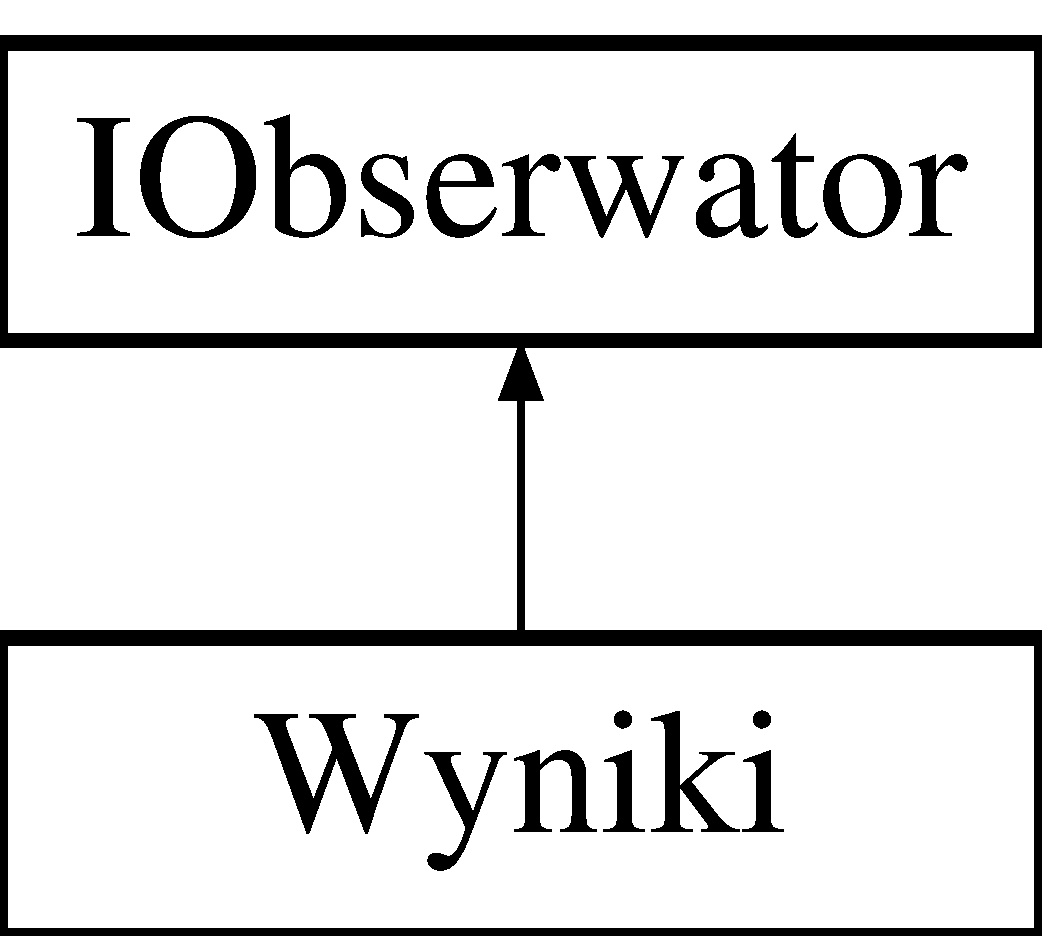
\includegraphics[height=2.000000cm]{class_wyniki}
\end{center}
\end{figure}
\subsection*{Public Member Functions}
\begin{DoxyCompactItemize}
\item 
\hyperlink{class_wyniki_a8d370dd59afbd516220a5abbfd5294be}{Wyniki} (const unsigned int Powtorzen, const unsigned int Proby, unsigned int $\ast$Rozmiary)
\item 
\hyperlink{class_wyniki_a0586d35f79012d9961cb4762567357c3}{$\sim$\-Wyniki} ()
\item 
void \hyperlink{class_wyniki_acc5e2bc728f9159a7e244339d84a47c6}{\-\_\-\-Zapisz\-Wyniki} (std\-::string Plik\-Wy) const 
\item 
void \hyperlink{class_wyniki_a4014236438f62cfd90c03de49ea38e5f}{\-\_\-\-Aktualizuj} ()
\begin{DoxyCompactList}\small\item\em Metoda Aktualizujaca stan. \end{DoxyCompactList}\end{DoxyCompactItemize}
\subsection*{Private Attributes}
\begin{DoxyCompactItemize}
\item 
unsigned int \hyperlink{class_wyniki_ac276b321edb9c38043e2b5aba213d847}{\-\_\-\-Ilosc\-Prob}
\item 
unsigned int \hyperlink{class_wyniki_ad207dabc5d9f03c957e1d023276f5548}{\-\_\-\-Ilosc\-Powtorzen}
\item 
unsigned int $\ast$ \hyperlink{class_wyniki_a559a3c3c4374708a493e8636320d9165}{\-\_\-\-Tablica\-Rozmiarow}
\item 
long double $\ast$ \hyperlink{class_wyniki_a6f47caedb424b964c117252febe1f135}{\-\_\-\-Tablica\-Wynikow}
\item 
\hyperlink{class_czasomierz}{Czasomierz} \hyperlink{class_wyniki_ac62ede680255427ef8f51e38e3eddcb9}{Stoper}
\end{DoxyCompactItemize}


\subsection{Constructor \& Destructor Documentation}
\hypertarget{class_wyniki_a8d370dd59afbd516220a5abbfd5294be}{\index{Wyniki@{Wyniki}!Wyniki@{Wyniki}}
\index{Wyniki@{Wyniki}!Wyniki@{Wyniki}}
\subsubsection[{Wyniki}]{\setlength{\rightskip}{0pt plus 5cm}Wyniki\-::\-Wyniki (
\begin{DoxyParamCaption}
\item[{const unsigned int}]{Powtorzen, }
\item[{const unsigned int}]{Proby, }
\item[{unsigned int $\ast$}]{Rozmiary}
\end{DoxyParamCaption}
)}}\label{class_wyniki_a8d370dd59afbd516220a5abbfd5294be}
\hypertarget{class_wyniki_a0586d35f79012d9961cb4762567357c3}{\index{Wyniki@{Wyniki}!$\sim$\-Wyniki@{$\sim$\-Wyniki}}
\index{$\sim$\-Wyniki@{$\sim$\-Wyniki}!Wyniki@{Wyniki}}
\subsubsection[{$\sim$\-Wyniki}]{\setlength{\rightskip}{0pt plus 5cm}Wyniki\-::$\sim$\-Wyniki (
\begin{DoxyParamCaption}
{}
\end{DoxyParamCaption}
)}}\label{class_wyniki_a0586d35f79012d9961cb4762567357c3}


\subsection{Member Function Documentation}
\hypertarget{class_wyniki_a4014236438f62cfd90c03de49ea38e5f}{\index{Wyniki@{Wyniki}!\-\_\-\-Aktualizuj@{\-\_\-\-Aktualizuj}}
\index{\-\_\-\-Aktualizuj@{\-\_\-\-Aktualizuj}!Wyniki@{Wyniki}}
\subsubsection[{\-\_\-\-Aktualizuj}]{\setlength{\rightskip}{0pt plus 5cm}void Wyniki\-::\-\_\-\-Aktualizuj (
\begin{DoxyParamCaption}
{}
\end{DoxyParamCaption}
)\hspace{0.3cm}{\ttfamily [virtual]}}}\label{class_wyniki_a4014236438f62cfd90c03de49ea38e5f}


Metoda Aktualizujaca stan. 

Metoda ma za zadanie poinformowac o zmianach w obiekcie ktory jest obserwowany 

Implements \hyperlink{class_i_obserwator_ab01d64a94e127100951aa287d4d2275f}{I\-Obserwator}.

\hypertarget{class_wyniki_acc5e2bc728f9159a7e244339d84a47c6}{\index{Wyniki@{Wyniki}!\-\_\-\-Zapisz\-Wyniki@{\-\_\-\-Zapisz\-Wyniki}}
\index{\-\_\-\-Zapisz\-Wyniki@{\-\_\-\-Zapisz\-Wyniki}!Wyniki@{Wyniki}}
\subsubsection[{\-\_\-\-Zapisz\-Wyniki}]{\setlength{\rightskip}{0pt plus 5cm}void Wyniki\-::\-\_\-\-Zapisz\-Wyniki (
\begin{DoxyParamCaption}
\item[{std\-::string}]{Plik\-Wy}
\end{DoxyParamCaption}
) const}}\label{class_wyniki_acc5e2bc728f9159a7e244339d84a47c6}


\subsection{Member Data Documentation}
\hypertarget{class_wyniki_ad207dabc5d9f03c957e1d023276f5548}{\index{Wyniki@{Wyniki}!\-\_\-\-Ilosc\-Powtorzen@{\-\_\-\-Ilosc\-Powtorzen}}
\index{\-\_\-\-Ilosc\-Powtorzen@{\-\_\-\-Ilosc\-Powtorzen}!Wyniki@{Wyniki}}
\subsubsection[{\-\_\-\-Ilosc\-Powtorzen}]{\setlength{\rightskip}{0pt plus 5cm}unsigned int Wyniki\-::\-\_\-\-Ilosc\-Powtorzen\hspace{0.3cm}{\ttfamily [private]}}}\label{class_wyniki_ad207dabc5d9f03c957e1d023276f5548}
\hypertarget{class_wyniki_ac276b321edb9c38043e2b5aba213d847}{\index{Wyniki@{Wyniki}!\-\_\-\-Ilosc\-Prob@{\-\_\-\-Ilosc\-Prob}}
\index{\-\_\-\-Ilosc\-Prob@{\-\_\-\-Ilosc\-Prob}!Wyniki@{Wyniki}}
\subsubsection[{\-\_\-\-Ilosc\-Prob}]{\setlength{\rightskip}{0pt plus 5cm}unsigned int Wyniki\-::\-\_\-\-Ilosc\-Prob\hspace{0.3cm}{\ttfamily [private]}}}\label{class_wyniki_ac276b321edb9c38043e2b5aba213d847}
\hypertarget{class_wyniki_a559a3c3c4374708a493e8636320d9165}{\index{Wyniki@{Wyniki}!\-\_\-\-Tablica\-Rozmiarow@{\-\_\-\-Tablica\-Rozmiarow}}
\index{\-\_\-\-Tablica\-Rozmiarow@{\-\_\-\-Tablica\-Rozmiarow}!Wyniki@{Wyniki}}
\subsubsection[{\-\_\-\-Tablica\-Rozmiarow}]{\setlength{\rightskip}{0pt plus 5cm}unsigned int$\ast$ Wyniki\-::\-\_\-\-Tablica\-Rozmiarow\hspace{0.3cm}{\ttfamily [private]}}}\label{class_wyniki_a559a3c3c4374708a493e8636320d9165}
\hypertarget{class_wyniki_a6f47caedb424b964c117252febe1f135}{\index{Wyniki@{Wyniki}!\-\_\-\-Tablica\-Wynikow@{\-\_\-\-Tablica\-Wynikow}}
\index{\-\_\-\-Tablica\-Wynikow@{\-\_\-\-Tablica\-Wynikow}!Wyniki@{Wyniki}}
\subsubsection[{\-\_\-\-Tablica\-Wynikow}]{\setlength{\rightskip}{0pt plus 5cm}long double$\ast$ Wyniki\-::\-\_\-\-Tablica\-Wynikow\hspace{0.3cm}{\ttfamily [private]}}}\label{class_wyniki_a6f47caedb424b964c117252febe1f135}
\hypertarget{class_wyniki_ac62ede680255427ef8f51e38e3eddcb9}{\index{Wyniki@{Wyniki}!Stoper@{Stoper}}
\index{Stoper@{Stoper}!Wyniki@{Wyniki}}
\subsubsection[{Stoper}]{\setlength{\rightskip}{0pt plus 5cm}{\bf Czasomierz} Wyniki\-::\-Stoper\hspace{0.3cm}{\ttfamily [private]}}}\label{class_wyniki_ac62ede680255427ef8f51e38e3eddcb9}


The documentation for this class was generated from the following files\-:\begin{DoxyCompactItemize}
\item 
/home/bartolomeo/209296/prj/inc/\hyperlink{_wyniki_8hh}{Wyniki.\-hh}\item 
/home/bartolomeo/209296/prj/src/\hyperlink{_wyniki_8cpp}{Wyniki.\-cpp}\end{DoxyCompactItemize}

\chapter{File Documentation}
\hypertarget{_benchmark_interfejs_8hh}{\section{/home/bartolomeo/209296/prj/inc/\-Benchmark\-Interfejs.hh File Reference}
\label{_benchmark_interfejs_8hh}\index{/home/bartolomeo/209296/prj/inc/\-Benchmark\-Interfejs.\-hh@{/home/bartolomeo/209296/prj/inc/\-Benchmark\-Interfejs.\-hh}}
}
{\ttfamily \#include $<$iostream$>$}\\*
{\ttfamily \#include $<$cstdlib$>$}\\*
{\ttfamily \#include $<$fstream$>$}\\*
{\ttfamily \#include $<$cstring$>$}\\*
{\ttfamily \#include $<$list$>$}\\*
{\ttfamily \#include \char`\"{}I\-Obserwowany.\-hh\char`\"{}}\\*
\subsection*{Classes}
\begin{DoxyCompactItemize}
\item 
class \hyperlink{class_benchmark_interfejs}{Benchmark\-Interfejs}
\begin{DoxyCompactList}\small\item\em Modeluje pojecie Interfejsu Benchmark'u. \end{DoxyCompactList}\end{DoxyCompactItemize}
\subsection*{Macros}
\begin{DoxyCompactItemize}
\item 
\#define \hyperlink{_benchmark_interfejs_8hh_ac6d08416f5bf3ac9d0a6c16e4885128c}{D\-L\-U\-G\-O\-S\-C\-\_\-\-S\-L\-O\-W\-A}~5
\end{DoxyCompactItemize}


\subsection{Macro Definition Documentation}
\hypertarget{_benchmark_interfejs_8hh_ac6d08416f5bf3ac9d0a6c16e4885128c}{\index{Benchmark\-Interfejs.\-hh@{Benchmark\-Interfejs.\-hh}!D\-L\-U\-G\-O\-S\-C\-\_\-\-S\-L\-O\-W\-A@{D\-L\-U\-G\-O\-S\-C\-\_\-\-S\-L\-O\-W\-A}}
\index{D\-L\-U\-G\-O\-S\-C\-\_\-\-S\-L\-O\-W\-A@{D\-L\-U\-G\-O\-S\-C\-\_\-\-S\-L\-O\-W\-A}!BenchmarkInterfejs.hh@{Benchmark\-Interfejs.\-hh}}
\subsubsection[{D\-L\-U\-G\-O\-S\-C\-\_\-\-S\-L\-O\-W\-A}]{\setlength{\rightskip}{0pt plus 5cm}\#define D\-L\-U\-G\-O\-S\-C\-\_\-\-S\-L\-O\-W\-A~5}}\label{_benchmark_interfejs_8hh_ac6d08416f5bf3ac9d0a6c16e4885128c}

\hypertarget{_czasomierz_8hh}{\section{/home/bartolomeo/209296/prj/inc/\-Czasomierz.hh File Reference}
\label{_czasomierz_8hh}\index{/home/bartolomeo/209296/prj/inc/\-Czasomierz.\-hh@{/home/bartolomeo/209296/prj/inc/\-Czasomierz.\-hh}}
}
{\ttfamily \#include $<$iostream$>$}\\*
{\ttfamily \#include $<$cstdlib$>$}\\*
{\ttfamily \#include $<$fstream$>$}\\*
{\ttfamily \#include $<$cstring$>$}\\*
\subsection*{Classes}
\begin{DoxyCompactItemize}
\item 
class \hyperlink{class_czasomierz}{Czasomierz}
\begin{DoxyCompactList}\small\item\em Modeluje pojecie Czasomierza. \end{DoxyCompactList}\end{DoxyCompactItemize}

\hypertarget{_h_sort_8hh}{\section{/home/bartolomeo/209296/prj/inc/\-H\-Sort.hh File Reference}
\label{_h_sort_8hh}\index{/home/bartolomeo/209296/prj/inc/\-H\-Sort.\-hh@{/home/bartolomeo/209296/prj/inc/\-H\-Sort.\-hh}}
}
{\ttfamily \#include \char`\"{}I\-Sortable.\-hh\char`\"{}}\\*
{\ttfamily \#include \char`\"{}Iterable.\-hh\char`\"{}}\\*
\subsection*{Classes}
\begin{DoxyCompactItemize}
\item 
class \hyperlink{class_h_sort}{H\-Sort$<$ Typ $>$}
\begin{DoxyCompactList}\small\item\em Modeluje sortowanie przez kopcowanie. \end{DoxyCompactList}\end{DoxyCompactItemize}

\hypertarget{_hyb_sort_8hh}{\section{/home/bartolomeo/209296/prj/inc/\-Hyb\-Sort.hh File Reference}
\label{_hyb_sort_8hh}\index{/home/bartolomeo/209296/prj/inc/\-Hyb\-Sort.\-hh@{/home/bartolomeo/209296/prj/inc/\-Hyb\-Sort.\-hh}}
}
{\ttfamily \#include \char`\"{}Q\-Sort\-Opt.\-hh\char`\"{}}\\*
{\ttfamily \#include \char`\"{}I\-Sortable.\-hh\char`\"{}}\\*
{\ttfamily \#include \char`\"{}Iterable.\-hh\char`\"{}}\\*
\subsection*{Classes}
\begin{DoxyCompactItemize}
\item 
class \hyperlink{class_hyb_sort}{Hyb\-Sort$<$ Typ $>$}
\begin{DoxyCompactList}\small\item\em Modeluje sortowania hybrydowego. \end{DoxyCompactList}\end{DoxyCompactItemize}
\subsection*{Macros}
\begin{DoxyCompactItemize}
\item 
\#define \hyperlink{_hyb_sort_8hh_a60a12235056da679c8976cec1faa66e2}{P\-R\-O\-G}~13
\item 
\#define \hyperlink{_hyb_sort_8hh_aa59719977f35b96c6798e939300c0a8f}{I\-L\-E}~3
\end{DoxyCompactItemize}


\subsection{Macro Definition Documentation}
\hypertarget{_hyb_sort_8hh_aa59719977f35b96c6798e939300c0a8f}{\index{Hyb\-Sort.\-hh@{Hyb\-Sort.\-hh}!I\-L\-E@{I\-L\-E}}
\index{I\-L\-E@{I\-L\-E}!HybSort.hh@{Hyb\-Sort.\-hh}}
\subsubsection[{I\-L\-E}]{\setlength{\rightskip}{0pt plus 5cm}\#define I\-L\-E~3}}\label{_hyb_sort_8hh_aa59719977f35b96c6798e939300c0a8f}
\hypertarget{_hyb_sort_8hh_a60a12235056da679c8976cec1faa66e2}{\index{Hyb\-Sort.\-hh@{Hyb\-Sort.\-hh}!P\-R\-O\-G@{P\-R\-O\-G}}
\index{P\-R\-O\-G@{P\-R\-O\-G}!HybSort.hh@{Hyb\-Sort.\-hh}}
\subsubsection[{P\-R\-O\-G}]{\setlength{\rightskip}{0pt plus 5cm}\#define P\-R\-O\-G~13}}\label{_hyb_sort_8hh_a60a12235056da679c8976cec1faa66e2}

\hypertarget{_i_obserwator_8hh}{\section{/home/bartolomeo/209296/prj/inc/\-I\-Obserwator.hh File Reference}
\label{_i_obserwator_8hh}\index{/home/bartolomeo/209296/prj/inc/\-I\-Obserwator.\-hh@{/home/bartolomeo/209296/prj/inc/\-I\-Obserwator.\-hh}}
}
\subsection*{Classes}
\begin{DoxyCompactItemize}
\item 
class \hyperlink{class_i_obserwator}{I\-Obserwator}
\begin{DoxyCompactList}\small\item\em Modeluje pojecie interfejsu dla obserwatora. \end{DoxyCompactList}\end{DoxyCompactItemize}

\hypertarget{_i_obserwowany_8hh}{\section{/home/bartolomeo/209296/prj/inc/\-I\-Obserwowany.hh File Reference}
\label{_i_obserwowany_8hh}\index{/home/bartolomeo/209296/prj/inc/\-I\-Obserwowany.\-hh@{/home/bartolomeo/209296/prj/inc/\-I\-Obserwowany.\-hh}}
}
{\ttfamily \#include $<$iostream$>$}\\*
{\ttfamily \#include \char`\"{}I\-Obserwator.\-hh\char`\"{}}\\*
\subsection*{Classes}
\begin{DoxyCompactItemize}
\item 
class \hyperlink{class_i_obserwowany}{I\-Obserwowany}
\begin{DoxyCompactList}\small\item\em Interfejs dla Obserwatora. \end{DoxyCompactList}\end{DoxyCompactItemize}

\hypertarget{_i_sortable_8hh}{\section{/home/bartolomeo/209296/prj/inc/\-I\-Sortable.hh File Reference}
\label{_i_sortable_8hh}\index{/home/bartolomeo/209296/prj/inc/\-I\-Sortable.\-hh@{/home/bartolomeo/209296/prj/inc/\-I\-Sortable.\-hh}}
}
{\ttfamily \#include \char`\"{}Iterable.\-hh\char`\"{}}\\*
\subsection*{Classes}
\begin{DoxyCompactItemize}
\item 
class \hyperlink{class_i_sortable}{I\-Sortable$<$ Typ $>$}
\begin{DoxyCompactList}\small\item\em Definicja klasy \hyperlink{class_i_sortable}{I\-Sortable}. \end{DoxyCompactList}\end{DoxyCompactItemize}

\hypertarget{_i_struktury_8hh}{\section{/home/bartolomeo/209296/prj/inc/\-I\-Struktury.hh File Reference}
\label{_i_struktury_8hh}\index{/home/bartolomeo/209296/prj/inc/\-I\-Struktury.\-hh@{/home/bartolomeo/209296/prj/inc/\-I\-Struktury.\-hh}}
}
{\ttfamily \#include $<$iostream$>$}\\*
{\ttfamily \#include $<$cstring$>$}\\*
{\ttfamily \#include $<$sstream$>$}\\*
{\ttfamily \#include $<$fstream$>$}\\*
\subsection*{Classes}
\begin{DoxyCompactItemize}
\item 
class \hyperlink{class_struktury}{Struktury$<$ Typ $>$}
\begin{DoxyCompactList}\small\item\em Modeluje pojecie \hyperlink{class_struktury}{Struktury} danych, klasa bazowa dla Stosu,Kolejki i Listy,zarowno w implemenetacji wskaznikowej jak i tablicowej. \end{DoxyCompactList}\end{DoxyCompactItemize}

\hypertarget{_iterable_8hh}{\section{/home/bartolomeo/209296/prj/inc/\-Iterable.hh File Reference}
\label{_iterable_8hh}\index{/home/bartolomeo/209296/prj/inc/\-Iterable.\-hh@{/home/bartolomeo/209296/prj/inc/\-Iterable.\-hh}}
}
\subsection*{Classes}
\begin{DoxyCompactItemize}
\item 
class \hyperlink{class_iterable}{Iterable$<$ Typ $>$}
\begin{DoxyCompactList}\small\item\em Interfejs \hyperlink{class_iterable}{Iterable}. \end{DoxyCompactList}\end{DoxyCompactItemize}

\hypertarget{_list_arr2x_8hh}{\section{/home/bartolomeo/209296/prj/inc/\-List\-Arr2x.hh File Reference}
\label{_list_arr2x_8hh}\index{/home/bartolomeo/209296/prj/inc/\-List\-Arr2x.\-hh@{/home/bartolomeo/209296/prj/inc/\-List\-Arr2x.\-hh}}
}


Definicja klasy List\-Arr1.  


{\ttfamily \#include \char`\"{}I\-Struktury.\-hh\char`\"{}}\\*
{\ttfamily \#include \char`\"{}Iterable.\-hh\char`\"{}}\\*
{\ttfamily \#include $<$fstream$>$}\\*
{\ttfamily \#include $<$cstdlib$>$}\\*
{\ttfamily \#include $<$cmath$>$}\\*
\subsection*{Classes}
\begin{DoxyCompactItemize}
\item 
class \hyperlink{class_list_arr2x}{List\-Arr2x$<$ Typ $>$}
\begin{DoxyCompactList}\small\item\em Modeluje pojęcie Listy (array) \end{DoxyCompactList}\end{DoxyCompactItemize}


\subsection{Detailed Description}
Definicja klasy List\-Arr1. Plik zawiera definicję klasy Lista\-Arr2x ujętej w szablon typu wraz z jej składowymi metofdami. 
\hypertarget{_m_sort_8hh}{\section{/home/bartolomeo/209296/prj/inc/\-M\-Sort.hh File Reference}
\label{_m_sort_8hh}\index{/home/bartolomeo/209296/prj/inc/\-M\-Sort.\-hh@{/home/bartolomeo/209296/prj/inc/\-M\-Sort.\-hh}}
}
{\ttfamily \#include \char`\"{}I\-Sortable.\-hh\char`\"{}}\\*
{\ttfamily \#include \char`\"{}Iterable.\-hh\char`\"{}}\\*
\subsection*{Classes}
\begin{DoxyCompactItemize}
\item 
class \hyperlink{class_m_sort}{M\-Sort$<$ Typ $>$}
\begin{DoxyCompactList}\small\item\em Modeluje sortowanie przez scalanie. \end{DoxyCompactList}\end{DoxyCompactItemize}

\hypertarget{_q_sort_8hh}{\section{/home/bartolomeo/209296/prj/inc/\-Q\-Sort.hh File Reference}
\label{_q_sort_8hh}\index{/home/bartolomeo/209296/prj/inc/\-Q\-Sort.\-hh@{/home/bartolomeo/209296/prj/inc/\-Q\-Sort.\-hh}}
}
{\ttfamily \#include \char`\"{}I\-Sortable.\-hh\char`\"{}}\\*
{\ttfamily \#include \char`\"{}Iterable.\-hh\char`\"{}}\\*
\subsection*{Classes}
\begin{DoxyCompactItemize}
\item 
class \hyperlink{class_q_sort}{Q\-Sort$<$ Typ $>$}
\begin{DoxyCompactList}\small\item\em Modeluje sortowanie szybkie. \end{DoxyCompactList}\end{DoxyCompactItemize}

\hypertarget{_q_sort_opt_8hh}{\section{/home/bartolomeo/209296/prj/inc/\-Q\-Sort\-Opt.hh File Reference}
\label{_q_sort_opt_8hh}\index{/home/bartolomeo/209296/prj/inc/\-Q\-Sort\-Opt.\-hh@{/home/bartolomeo/209296/prj/inc/\-Q\-Sort\-Opt.\-hh}}
}
{\ttfamily \#include \char`\"{}I\-Sortable.\-hh\char`\"{}}\\*
{\ttfamily \#include \char`\"{}Iterable.\-hh\char`\"{}}\\*
\subsection*{Classes}
\begin{DoxyCompactItemize}
\item 
class \hyperlink{class_q_sort_opt}{Q\-Sort\-Opt$<$ Typ $>$}
\begin{DoxyCompactList}\small\item\em Modeluje sortowanie szybkie z optymalizacja. \end{DoxyCompactList}\end{DoxyCompactItemize}
\subsection*{Macros}
\begin{DoxyCompactItemize}
\item 
\#define \hyperlink{_q_sort_opt_8hh_aa59719977f35b96c6798e939300c0a8f}{I\-L\-E}~3
\end{DoxyCompactItemize}


\subsection{Macro Definition Documentation}
\hypertarget{_q_sort_opt_8hh_aa59719977f35b96c6798e939300c0a8f}{\index{Q\-Sort\-Opt.\-hh@{Q\-Sort\-Opt.\-hh}!I\-L\-E@{I\-L\-E}}
\index{I\-L\-E@{I\-L\-E}!QSortOpt.hh@{Q\-Sort\-Opt.\-hh}}
\subsubsection[{I\-L\-E}]{\setlength{\rightskip}{0pt plus 5cm}\#define I\-L\-E~3}}\label{_q_sort_opt_8hh_aa59719977f35b96c6798e939300c0a8f}

\hypertarget{_stos_tab_8hh}{\section{/home/bartolomeo/209296/prj/inc/\-Stos\-Tab.hh File Reference}
\label{_stos_tab_8hh}\index{/home/bartolomeo/209296/prj/inc/\-Stos\-Tab.\-hh@{/home/bartolomeo/209296/prj/inc/\-Stos\-Tab.\-hh}}
}
{\ttfamily \#include $<$cstdlib$>$}\\*
{\ttfamily \#include $<$iostream$>$}\\*
{\ttfamily \#include \char`\"{}I\-Struktury.\-hh\char`\"{}}\\*
{\ttfamily \#include \char`\"{}Iterable.\-hh\char`\"{}}\\*
\subsection*{Classes}
\begin{DoxyCompactItemize}
\item 
class \hyperlink{class_stos_tab}{Stos\-Tab$<$ Typ $>$}
\end{DoxyCompactItemize}

\hypertarget{_struktury_benchmark_8hh}{\section{/home/bartolomeo/209296/prj/inc/\-Struktury\-Benchmark.hh File Reference}
\label{_struktury_benchmark_8hh}\index{/home/bartolomeo/209296/prj/inc/\-Struktury\-Benchmark.\-hh@{/home/bartolomeo/209296/prj/inc/\-Struktury\-Benchmark.\-hh}}
}
{\ttfamily \#include \char`\"{}Benchmark\-Interfejs.\-hh\char`\"{}}\\*
{\ttfamily \#include \char`\"{}I\-Sortable.\-hh\char`\"{}}\\*
{\ttfamily \#include \char`\"{}I\-Obserwowany.\-hh\char`\"{}}\\*
{\ttfamily \#include \char`\"{}I\-Struktury.\-hh\char`\"{}}\\*
\subsection*{Classes}
\begin{DoxyCompactItemize}
\item 
class \hyperlink{class_struktury_benchmark}{Struktury\-Benchmark$<$ Typ $>$}
\end{DoxyCompactItemize}

\hypertarget{_wyniki_8hh}{\section{/home/bartolomeo/209296/prj/inc/\-Wyniki.hh File Reference}
\label{_wyniki_8hh}\index{/home/bartolomeo/209296/prj/inc/\-Wyniki.\-hh@{/home/bartolomeo/209296/prj/inc/\-Wyniki.\-hh}}
}
{\ttfamily \#include $<$iostream$>$}\\*
{\ttfamily \#include \char`\"{}I\-Obserwator.\-hh\char`\"{}}\\*
{\ttfamily \#include \char`\"{}Czasomierz.\-hh\char`\"{}}\\*
{\ttfamily \#include $<$fstream$>$}\\*
{\ttfamily \#include $<$cstdlib$>$}\\*
{\ttfamily \#include $<$string$>$}\\*
\subsection*{Classes}
\begin{DoxyCompactItemize}
\item 
class \hyperlink{class_wyniki}{Wyniki}
\end{DoxyCompactItemize}

\hypertarget{_czasomierz_8cpp}{\section{/home/bartolomeo/209296/prj/src/\-Czasomierz.cpp File Reference}
\label{_czasomierz_8cpp}\index{/home/bartolomeo/209296/prj/src/\-Czasomierz.\-cpp@{/home/bartolomeo/209296/prj/src/\-Czasomierz.\-cpp}}
}
{\ttfamily \#include \char`\"{}Czasomierz.\-hh\char`\"{}}\\*

\hypertarget{_main_8cpp}{\section{/home/bartolomeo/209296/prj/src/\-Main.cpp File Reference}
\label{_main_8cpp}\index{/home/bartolomeo/209296/prj/src/\-Main.\-cpp@{/home/bartolomeo/209296/prj/src/\-Main.\-cpp}}
}


funkcja glowna programu  


{\ttfamily \#include \char`\"{}Struktury\-Benchmark.\-hh\char`\"{}}\\*
{\ttfamily \#include \char`\"{}Wyniki.\-hh\char`\"{}}\\*
{\ttfamily \#include \char`\"{}H\-Sort.\-hh\char`\"{}}\\*
{\ttfamily \#include \char`\"{}Hyb\-Sort.\-hh\char`\"{}}\\*
{\ttfamily \#include \char`\"{}List\-Arr2x.\-hh\char`\"{}}\\*
{\ttfamily \#include \char`\"{}M\-Sort.\-hh\char`\"{}}\\*
{\ttfamily \#include \char`\"{}Q\-Sort.\-hh\char`\"{}}\\*
{\ttfamily \#include \char`\"{}Q\-Sort\-Opt.\-hh\char`\"{}}\\*
{\ttfamily \#include \char`\"{}Stos\-Tab.\-hh\char`\"{}}\\*
\subsection*{Macros}
\begin{DoxyCompactItemize}
\item 
\#define \hyperlink{_main_8cpp_aba41c0aa9e20262fb937b6b958de59e2}{I\-L\-O\-S\-C\-\_\-\-P\-O\-W}~10
\item 
\#define \hyperlink{_main_8cpp_a345eda6ce2b2009daa29315332defd2a}{I\-L\-O\-S\-C\-\_\-\-P\-R\-O\-B}~5
\end{DoxyCompactItemize}
\subsection*{Functions}
\begin{DoxyCompactItemize}
\item 
int \hyperlink{_main_8cpp_ae66f6b31b5ad750f1fe042a706a4e3d4}{main} ()
\end{DoxyCompactItemize}
\subsection*{Variables}
\begin{DoxyCompactItemize}
\item 
unsigned int \hyperlink{_main_8cpp_a78d5bcfc9aaa29813c71793226e019cf}{Tablica\-\_\-\-Rozmiarow} \mbox{[}$\,$\mbox{]} = \{100,1000,10000,100000,1000000\}
\end{DoxyCompactItemize}


\subsection{Detailed Description}
funkcja glowna programu 

\subsection{Macro Definition Documentation}
\hypertarget{_main_8cpp_aba41c0aa9e20262fb937b6b958de59e2}{\index{Main.\-cpp@{Main.\-cpp}!I\-L\-O\-S\-C\-\_\-\-P\-O\-W@{I\-L\-O\-S\-C\-\_\-\-P\-O\-W}}
\index{I\-L\-O\-S\-C\-\_\-\-P\-O\-W@{I\-L\-O\-S\-C\-\_\-\-P\-O\-W}!Main.cpp@{Main.\-cpp}}
\subsubsection[{I\-L\-O\-S\-C\-\_\-\-P\-O\-W}]{\setlength{\rightskip}{0pt plus 5cm}\#define I\-L\-O\-S\-C\-\_\-\-P\-O\-W~10}}\label{_main_8cpp_aba41c0aa9e20262fb937b6b958de59e2}
\hypertarget{_main_8cpp_a345eda6ce2b2009daa29315332defd2a}{\index{Main.\-cpp@{Main.\-cpp}!I\-L\-O\-S\-C\-\_\-\-P\-R\-O\-B@{I\-L\-O\-S\-C\-\_\-\-P\-R\-O\-B}}
\index{I\-L\-O\-S\-C\-\_\-\-P\-R\-O\-B@{I\-L\-O\-S\-C\-\_\-\-P\-R\-O\-B}!Main.cpp@{Main.\-cpp}}
\subsubsection[{I\-L\-O\-S\-C\-\_\-\-P\-R\-O\-B}]{\setlength{\rightskip}{0pt plus 5cm}\#define I\-L\-O\-S\-C\-\_\-\-P\-R\-O\-B~5}}\label{_main_8cpp_a345eda6ce2b2009daa29315332defd2a}


\subsection{Function Documentation}
\hypertarget{_main_8cpp_ae66f6b31b5ad750f1fe042a706a4e3d4}{\index{Main.\-cpp@{Main.\-cpp}!main@{main}}
\index{main@{main}!Main.cpp@{Main.\-cpp}}
\subsubsection[{main}]{\setlength{\rightskip}{0pt plus 5cm}int main (
\begin{DoxyParamCaption}
{}
\end{DoxyParamCaption}
)}}\label{_main_8cpp_ae66f6b31b5ad750f1fe042a706a4e3d4}


\subsection{Variable Documentation}
\hypertarget{_main_8cpp_a78d5bcfc9aaa29813c71793226e019cf}{\index{Main.\-cpp@{Main.\-cpp}!Tablica\-\_\-\-Rozmiarow@{Tablica\-\_\-\-Rozmiarow}}
\index{Tablica\-\_\-\-Rozmiarow@{Tablica\-\_\-\-Rozmiarow}!Main.cpp@{Main.\-cpp}}
\subsubsection[{Tablica\-\_\-\-Rozmiarow}]{\setlength{\rightskip}{0pt plus 5cm}unsigned int Tablica\-\_\-\-Rozmiarow\mbox{[}$\,$\mbox{]} = \{100,1000,10000,100000,1000000\}}}\label{_main_8cpp_a78d5bcfc9aaa29813c71793226e019cf}

\hypertarget{_wyniki_8cpp}{\section{/home/bartolomeo/209296/prj/src/\-Wyniki.cpp File Reference}
\label{_wyniki_8cpp}\index{/home/bartolomeo/209296/prj/src/\-Wyniki.\-cpp@{/home/bartolomeo/209296/prj/src/\-Wyniki.\-cpp}}
}
{\ttfamily \#include \char`\"{}Wyniki.\-hh\char`\"{}}\\*

%--- End generated contents ---

% Index
\newpage
\phantomsection
\addcontentsline{toc}{chapter}{Index}
\printindex

\end{document}
